\def\figpath{tex/2_LC-Oszillator/pictures}
\graphicspath{{tex/2_LC-Oszillator/pictures/}}

\chapter{LC-Oszillator}
Das 2. Kapitel behandelt die Analyse der in Abb. \ref{fig_Kap2_01:Oszillator} gezeigten Oszillatorschaltung.

\begin{figure}[H]
    \centering
    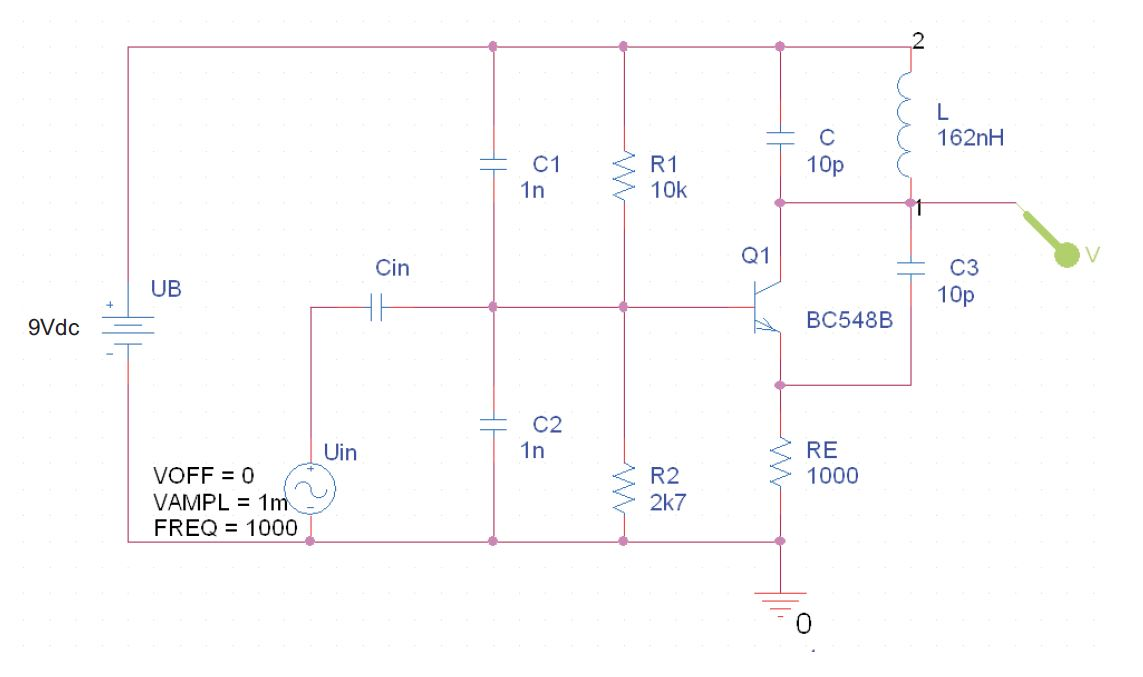
\includegraphics[width = \textwidth]{\figpath/Oszillatorschaltung.jpg}
    \caption{Oszillatorschaltung}
    \label{fig_Kap2_01:Oszillator}
\end{figure}

\section{Schwingbedingung}
Zuerst soll auf Basis des Kleinsignalersatzschaltbildes die Resonanzfrequenz berechnet werden. Hierbei dürfen lt. Praktikumsskript die Kapazitäten $C_1$ und $C_2$ als unendlich angenommen werden. Außerdem sind die parasitären Kapazitäten des Transistors lt. Abb. \ref{fig_Kap2_02:parasit} zu berücksichtigen.

\begin{figure}[H]
    \centering
    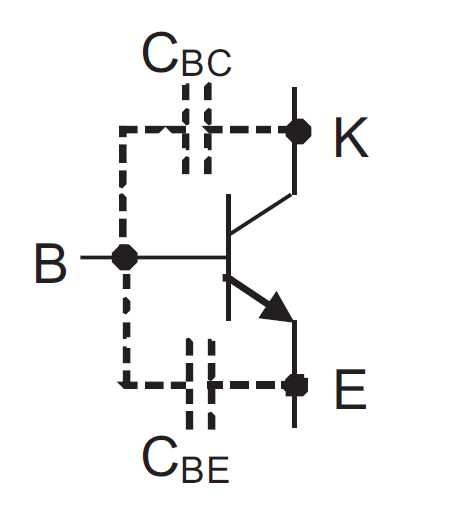
\includegraphics[width = 0.3\textwidth]{\figpath/parasit.jpg}
    \caption{Oszillatorschaltung}
    \label{fig_Kap2_02:parasit}
\end{figure}

Das KSESB der Oszillatorschaltung sieht folgendermaßen aus:

\begin{figure}[H]
	\centering
	\def\svgwidth{0.8\textwidth}
	\input{\figpath/KSESB.pdf_tex}
	\caption{KSESB der Oszillatorschaltung} 
	\label{fig:01_QStatAufbau} 
\end{figure}

Fasst man die relevanten Bauteile zu zwei Ersatzimpendazen

\begin{equation}
    \underline{Z}_1 = \frac{1}{\underline{Y}_1} = \frac{1}{\frac{S}{B}+\frac{1}{R_E}+j  \omega C_{BE}}
\end{equation}

\begin{equation}
    \underline{Z}_2 = \frac{1}{\underline{Y}_2} = \frac{1}{\frac{1}{j\omega L}+j \omega \left( C_{BC} + C \right)}
\end{equation}

zusammen, so lässt sich die Schaltung vereinfacht darstellen:

\begin{figure}[H]
	\centering
	\def\svgwidth{0.6\textwidth}
	\input{\figpath/KSESB2.pdf_tex}
	\caption{Vereinfachtes KSESB der Oszillatorschaltung} 
	\label{fig:01_QStatAufbau} 
\end{figure}

Laut der Kirchhoffschen Maschenregel kann nun folgender Ausdruck gebildet werden:

\begin{equation}
    u_{BE} \cdot \left( 1 + \frac{S + \underline{Y}_1}{j \omega C_3} + \frac{\underline{Y}_1}{\underline{Y}_2} \right) = 0
\end{equation}

Setzt man nun die Ausdrücke der Ersatzadmittanzen ein folgt:
\begin{equation}
    u_{BE} \cdot \left( 1 + \frac{S + \frac{S}{B}+\frac{1}{R_E}+j  \omega C_{BE}}{j \omega C_3} + \frac{\frac{S}{B}+\frac{1}{R_E}+j  \omega C_{BE}}{\frac{1}{j\omega L}+j \omega \left( C_{BC} + C \right)} \right) = 0
\end{equation}

Die Steuergröße des Oszillators, die Basis-Emitterspannung $u_{BE}$, darf naturgemäß nicht verschwinden, womit sich die Schwingbedingung im komplexen Zahlenraum ergibt:

\begin{equation}
    1 + \frac{S + \frac{S}{B}+\frac{1}{R_E}+j  \omega C_{BE}}{j \omega C_3} + \frac{\frac{S}{B}+\frac{1}{R_E}+j  \omega C_{BE}}{\frac{1}{j\omega L}+j \omega \left( C_{BC} + C \right)} = 0
\end{equation}

Betrachtet man nun den Real- und Imaginärteil obiger Gleichung einzeln, erhält man 2 reelle Schwingbedingungen, was mithilfe des Computeralgebraprogramms \textit{MAXIMA} hergeleitet wurde.\\
Für den Realteil gilt:

\begin{equation}
\label{glng_01}
    1 + \frac{C_{BE}\omega}{\omega (C_{BC} + C) - \frac{1}{\omega L}} + \frac{C_{BE}}{C_3} = 0
\end{equation}

Für den Imaginärteil ergibt sich folgende Gleichung:
\begin{equation}
    \label{glng_03}
    -\frac{\frac{S}{B}+\frac{1}{R_E}}{\omega(C_{BC} + C)-\frac{1}{\omega L}} - \frac{S\left(\frac{1}{B} + 1\right) + \frac{1}{R_E}}{\omega C_3} = 0
\end{equation}

Der variable Emitterwiderstand $R_E$ kommt in Gleichung \ref{glng_01} nicht vor, wodurch sich ein Ausdruck für die Resonanzkreisfrequenz aus einer quadratischen Gleichung finden lässt, wobei natürlich die negative Lösung verworfen wird: 

\begin{equation}
    \label{glng_02}
    \omega = \sqrt{\frac{C_{BE} + C_3}{\left( \left( C_{BC} + C_3 + C\right)C_{BE} + C_3 C_{BC} + CC_3 \right) L}}
\end{equation}

Setzt man nun die Lösung \ref{glng_02} in Gleichung \ref{glng_03} ein, lässt sich ein Ausdruck für den variablen Widerstand $R_E$ in Abhängigkeit der Steilheit $S$ des Transistors im jeweiligen Arbeitspunkt finden:

\begin{equation}
    R_E = \frac{B \cdot C_3}{S \cdot \left( B C_{BE} - C_3\right)}
\end{equation}

In Tab. \ref{tab_Kap2_01:Bauteilwerte} werden die aus dem in Abb. \ref{fig_Kap2_01:Oszillator} gezeigten Schematic verwendeten Bauteilwerte und Werte der Versorgungsspannung aufgelistet. Für die parasitären Kapazitäten $C_{BE}$ und $C_{BC}$ wurden für die Berechnung die approximierten Werte aus dem Skriptum verwendet.

\begin{table}[H]
\centering
\begin{tabular}{|c|c|} \hline
Benennung & Größe \\ \hline
$U_B$ & \SI{9}{\volt} \\ \hline
$C$ & \SI{9}{\volt} \\ \hline
$C_1$ & \SI{1}{\nano\farad} \\ \hline
$C_2$ & \SI{1}{\nano\farad} \\ \hline
$C_3$ & \SI{10}{\pico\farad} \\ \hline
$C_{BC}$ & \SI{5}{\pico\farad} \\ \hline
$C_{BE}$ & \SI{10}{\pico\farad} \\ \hline
$L$ & \SI{162}{\nano\henry} \\ \hline
$R_1$ & \SI{10}{\kilo\ohm} \\ \hline
$R_2$ & \SI{2.7}{\kilo\ohm} \\ \hline
$R_E$ & \SI{1}{\kilo\ohm} \\ \hline

\end{tabular}
\caption{Bauteilwerte für Berechnung und Simulation}
\label{tab_Kap2_01:Bauteilwerte} 
\end{table}

Diese Werte in Gleichung \ref{glng_02} eingesetzt, ergeben die Resonanzkreisfrequenz bzw. Frequenz von:

\begin{equation}
    \omega = \SI{555.5}{\mega \radian \per \second}
\end{equation}

\begin{equation}
    f = \frac{\omega}{2 \cdot \pi} = \frac{\SI{555.5}{\mega \radian \per \second}}{2 \cdot \pi} = \SI{88.42}{\mega \hertz}
\end{equation}


\section{Simulation}
Das Schematic laut Abbildung \ref{fig_Kap2_05:LTSpiceSchematic} wurde in LTSpice nachgebildet.

\begin{figure}[H]
    \centering
    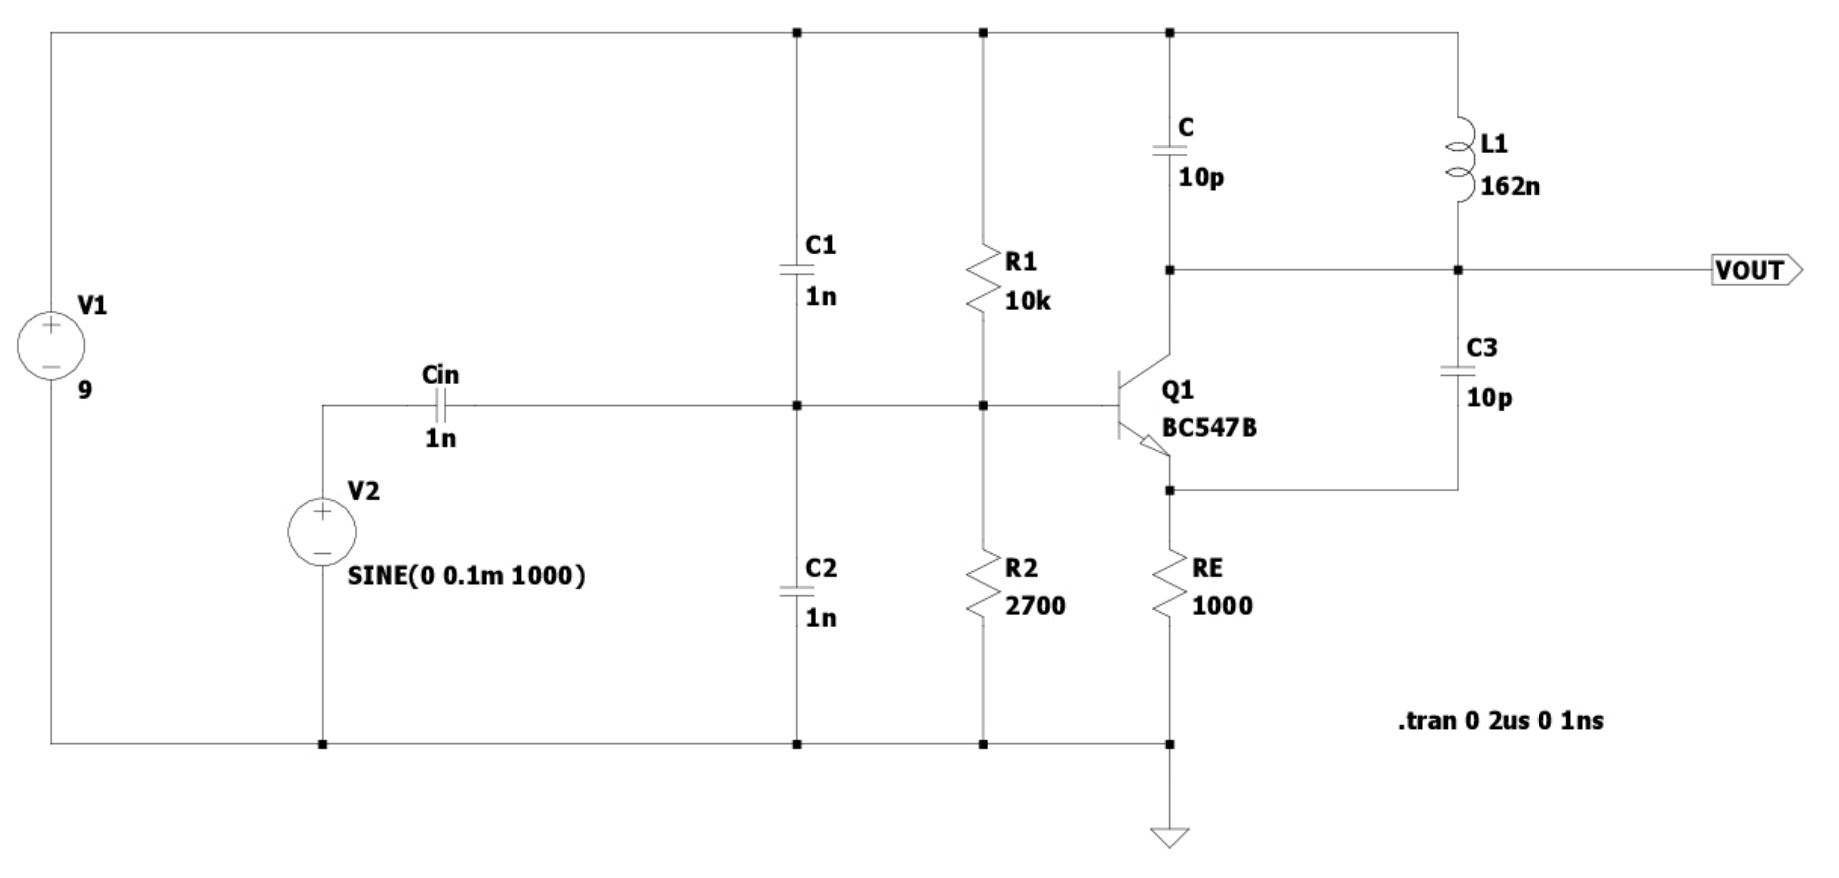
\includegraphics[width = \textwidth]{\figpath/LC_Oszillator_LTSpice.jpg}
    \caption{Oszillatorschaltung}
    \label{fig_Kap2_05:LTSpiceSchematic}
\end{figure}

Abbildung \ref{fig_Kap2_06:Einschw} zeigt den Einschwingvorgang der Oszillatorschaltung von 0 bis $\SI{2}{\micro\second}$. 

\begin{figure}[H]
	\centering \small
	% This file was created by matlab2tikz.
%
\definecolor{mycolor1}{rgb}{0.00000,0.44700,0.74100}%
%
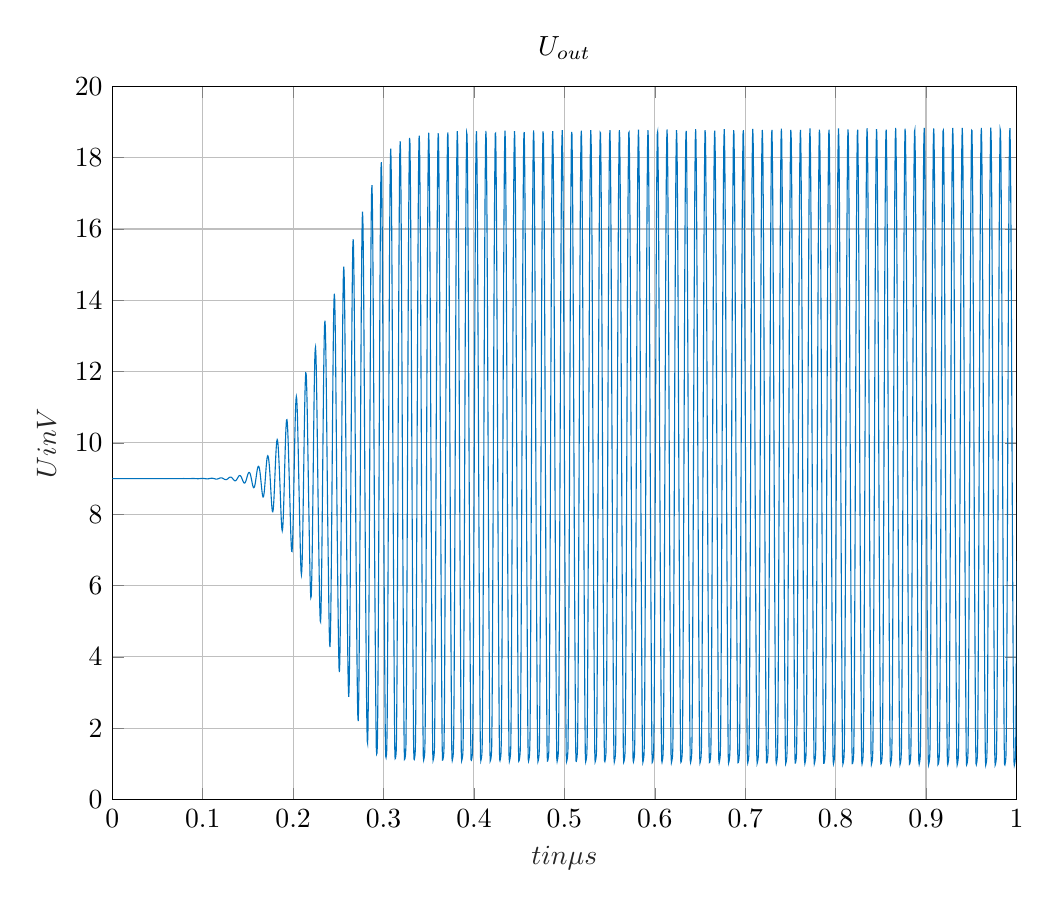
\begin{tikzpicture}

\begin{axis}[%
width=4.521in,
height=3.566in,
at={(0.758in,0.481in)},
scale only axis,
xmin=0,
xmax=1,
xlabel style={font=\color{white!15!black}},
xlabel={$t \text{ in } \mu\text{s}$},
ymin=0,
ymax=20,
ylabel style={font=\color{white!15!black}},
ylabel={$U \text{ in } \text{V}$},
axis background/.style={fill=white},
title style={font=\bfseries},
title={$U_{out}$},
xmajorgrids,
ymajorgrids
]
\addplot [color=mycolor1, forget plot]
  table[row sep=crcr]{%
0	8.999999\\
0.0004	8.99999838967629\\
0.0008	8.99999686569654\\
0.0012	8.99999523015525\\
0.0016	8.99999411302981\\
0.002	8.99999396378929\\
0.0024	8.99999496183693\\
0.0028	8.99999600004309\\
0.0032	8.99999601144986\\
0.0036	8.99999688080587\\
0.004	8.99999856890744\\
0.0044	9.00000016872829\\
0.0048	9.00000197820698\\
0.0052	9.00000302462223\\
0.0056	9.00000400868404\\
0.006	9.00000514301899\\
0.0064	9.00000595834729\\
0.0068	9.00000589649069\\
0.0072	9.00000603790676\\
0.0076	9.00000621288351\\
0.008	9.00000517191946\\
0.0084	9.00000304253182\\
0.0088	9.0000018021926\\
0.0092	8.99999899830263\\
0.0096	8.99999703268898\\
0.01	8.99999505774966\\
0.0104	8.99999291933071\\
0.0108	8.99999102858481\\
0.0112	8.99999000692144\\
0.0116	8.99998913023014\\
0.012	8.99998797428823\\
0.0124	8.99998899675239\\
0.0128	8.99998924082774\\
0.0132	8.99999049021926\\
0.0136	8.99999308724682\\
0.014	8.99999474065089\\
0.0144	9.00001886641445\\
0.0148	9.00000078360073\\
0.0152	9.00000506388139\\
0.0156	9.00000780168504\\
0.016	9.00001060148523\\
0.0164	9.00001109073879\\
0.0168	9.00001299399985\\
0.0172	9.0000139838877\\
0.0176	9.00001371792252\\
0.018	9.00001210905346\\
0.0184	9.00001005344526\\
0.0188	9.00000627490923\\
0.0192	9.00000325663169\\
0.0196	8.99999878307638\\
0.02	8.99999419379834\\
0.0204	8.99999016965786\\
0.0208	8.99998530459073\\
0.0212	8.99998193485678\\
0.0216	8.99997918849263\\
0.022	8.99997786688224\\
0.0224	8.99997691658306\\
0.0228	8.99997800355401\\
0.0232	8.99997959534509\\
0.0236	8.99998332216269\\
0.024	8.99998743284493\\
0.0244	8.99999286129744\\
0.0248	8.99999830483027\\
0.0252	9.00000472292231\\
0.0256	9.00001110799464\\
0.026	9.00001774906111\\
0.0264	9.00002249826569\\
0.0268	9.0000263967145\\
0.0272	9.00002901917139\\
0.0276	9.00003001621248\\
0.028	9.00002855248071\\
0.0284	9.00002581522651\\
0.0288	9.00002094507612\\
0.0292	9.00001382436087\\
0.0296	9.00000613067045\\
0.03	8.99999725769229\\
0.0304	8.99998813479444\\
0.0308	8.99997925279779\\
0.0312	8.99997062231366\\
0.0316	8.99996349759487\\
0.032	8.99995815201829\\
0.0324	8.99995539083545\\
0.0328	8.99995396178781\\
0.0332	8.99995607660858\\
0.0336	8.99996051400527\\
0.034	8.99996771691482\\
0.0344	8.99997721441343\\
0.0348	8.99999000668954\\
0.0352	9.00000203437561\\
0.0356	9.00001531139778\\
0.036	9.00002829966293\\
0.0364	9.00003989241786\\
0.0368	9.00005064481728\\
0.0372	9.0000577647402\\
0.0376	9.00006219333106\\
0.038	9.00006303795749\\
0.0384	9.00005976212627\\
0.0388	9.00005244687302\\
0.0392	9.00004152491632\\
0.0396	9.00002688313883\\
0.04	9.0000108378787\\
0.0404	8.99999174163512\\
0.0408	8.99997256348102\\
0.0412	8.99995431046423\\
0.0416	8.99993773570619\\
0.042	8.99992446527001\\
0.0424	8.99991403970436\\
0.0428	8.99990739035776\\
0.0432	8.99990741904298\\
0.0436	8.99991271573695\\
0.044	8.99992399472344\\
0.0444	8.99993956735001\\
0.0448	8.99995980536268\\
0.0452	8.99998543777458\\
0.0456	9.00001073944847\\
0.046	9.00003969583468\\
0.0464	9.00006493268627\\
0.0468	9.00008851105272\\
0.0472	9.00010824591375\\
0.0476	9.00012230320767\\
0.048	9.00012971327617\\
0.0484	9.00012959470454\\
0.0488	9.00012137682707\\
0.0492	9.00010433236284\\
0.0496	9.00008084303201\\
0.05	9.00004986845586\\
0.0504	9.00001927272659\\
0.0508	8.99997696434652\\
0.0512	8.99993954005854\\
0.0516	8.9999006014023\\
0.052	8.99986767962768\\
0.0524	8.99983832286559\\
0.0528	8.99982009841632\\
0.0532	8.99981001147231\\
0.0536	8.99981149637292\\
0.054	8.99982410055916\\
0.0544	8.99984919100181\\
0.0548	8.99988443291931\\
0.0552	8.99993162958653\\
0.0556	8.99998017363469\\
0.056	9.00003523639594\\
0.0564	9.00008929322112\\
0.0568	9.0001452335748\\
0.0572	9.00018481081138\\
0.0576	9.00023097514892\\
0.058	9.00025721603845\\
0.0584	9.00026965833924\\
0.0588	9.00026540920275\\
0.0592	9.00024605323511\\
0.0596	9.00020717841248\\
0.06	9.00015643204338\\
0.0604	9.00009294904116\\
0.0608	9.0000176167264\\
0.0612	8.99994014238327\\
0.0616	8.99985697640782\\
0.062	8.99978269939909\\
0.0624	8.99971109031033\\
0.0628	8.99966085466284\\
0.0632	8.99962557027203\\
0.0636	8.99961043756331\\
0.064	8.99961810458076\\
0.0644	8.99964983608158\\
0.0648	8.99970472727935\\
0.0652	8.99978108709992\\
0.0656	8.99987542196792\\
0.066	8.99998273771292\\
0.0664	9.00009695457627\\
0.0668	9.0002138790425\\
0.0672	9.00032034015708\\
0.0676	9.00041040911187\\
0.068	9.00049061006277\\
0.0684	9.00053803271473\\
0.0688	9.0005560558257\\
0.0692	9.00054249698722\\
0.0696	9.00049147502464\\
0.07	9.00041035609155\\
0.0704	9.00029808706227\\
0.0708	9.00015908600352\\
0.0712	9.00000570287915\\
0.0716	8.9998560500597\\
0.072	8.99967467177258\\
0.0724	8.99952469730375\\
0.0728	8.9993899752497\\
0.0732	8.99928572201121\\
0.0736	8.99922012775065\\
0.074	8.99919802897446\\
0.0744	8.99922512673306\\
0.0748	8.99929772360742\\
0.0752	8.99942386766052\\
0.0756	8.99958808769171\\
0.076	8.99979269792521\\
0.0764	9.00001257595628\\
0.0768	9.00024025311668\\
0.0772	9.00048491597225\\
0.0776	9.00070185304272\\
0.078	9.00089050231541\\
0.0784	9.00103341888302\\
0.0788	9.00112155201448\\
0.0792	9.00114528540155\\
0.0796	9.00110058646342\\
0.08	9.00098353440148\\
0.0804	9.00080220823286\\
0.0808	9.00055970313146\\
0.0812	9.00026706407757\\
0.0816	8.99994605353863\\
0.082	8.99960025083228\\
0.0824	8.9992696523709\\
0.0828	8.99896465275298\\
0.0832	8.99869558500436\\
0.0836	8.99849892282032\\
0.084	8.99838133828622\\
0.0844	8.99835634533498\\
0.0848	8.99843042083415\\
0.0852	8.99860579674798\\
0.0856	8.99887604416635\\
0.086	8.99923365515104\\
0.0864	8.99965941541832\\
0.0868	9.00012196224281\\
0.0872	9.00061636812878\\
0.0876	9.00109150122183\\
0.088	9.00153107400185\\
0.0884	9.00189904620356\\
0.0888	9.00217374136239\\
0.0892	9.00232929334603\\
0.0896	9.00234920410569\\
0.09	9.00222815750158\\
0.0904	9.00196135589972\\
0.0908	9.00156028545291\\
0.0912	9.00103618420395\\
0.0916	9.00042250762539\\
0.092	8.99974848438237\\
0.0924	8.99903835081215\\
0.0928	8.99836876484343\\
0.0932	8.99773547981606\\
0.0936	8.99722601461112\\
0.094	8.99684847317128\\
0.0944	8.99664377757037\\
0.0948	8.99663373888126\\
0.0952	8.99682968256149\\
0.0956	8.99723305375093\\
0.096	8.99782603985625\\
0.0964	8.99860395662605\\
0.0968	8.99948591268397\\
0.0972	9.00045011180936\\
0.0976	9.00147223686242\\
0.098	9.00243396666284\\
0.0984	9.00331681572358\\
0.0988	9.0040398086674\\
0.0992	9.00455570873867\\
0.0996	9.00482211664915\\
0.1	9.00480630977396\\
0.1004	9.00449334712945\\
0.1008	9.00388932299256\\
0.1012	9.00301063847443\\
0.1016	9.00188413819504\\
0.102	9.00060171935143\\
0.1024	8.99919757966046\\
0.1028	8.99774351547753\\
0.1032	8.99637686207387\\
0.1036	8.99512185446846\\
0.104	8.99411033907828\\
0.1044	8.99340152714396\\
0.1048	8.99306020087162\\
0.1052	8.99312551786131\\
0.1056	8.99361578246248\\
0.106	8.99452833276431\\
0.1064	8.99583252632719\\
0.1068	8.99747679774845\\
0.1072	8.99933552515082\\
0.1076	9.00138586253856\\
0.108	9.00343967258295\\
0.1084	9.00539470162953\\
0.1088	9.00715244769382\\
0.1092	9.00855960592333\\
0.1096	9.0095233110054\\
0.11	9.00995429406231\\
0.1104	9.00980142932306\\
0.1108	9.00903490118392\\
0.1112	9.0076765952399\\
0.1116	9.00576240511009\\
0.112	9.00337220296459\\
0.1124	9.00067333547917\\
0.1128	8.99771150487114\\
0.1132	8.9947868788714\\
0.1136	8.99196405735839\\
0.114	8.98950421904934\\
0.1144	8.98753333724339\\
0.1148	8.98621707426336\\
0.1152	8.98567914050207\\
0.1156	8.9859902791465\\
0.116	8.9871859704585\\
0.1164	8.98923643535148\\
0.1168	8.99206765783106\\
0.1172	8.99555474544451\\
0.1176	8.99947659323449\\
0.118	9.00374136637521\\
0.1184	9.00790201833104\\
0.1188	9.01188758930009\\
0.1192	9.01535042870712\\
0.1196	9.01807603694608\\
0.12	9.01984278407808\\
0.1204	9.02049297473739\\
0.1208	9.01992571323013\\
0.1212	9.01810633548913\\
0.1216	9.01506864206408\\
0.122	9.01089790028544\\
0.1224	9.00589005011968\\
0.1228	9.00018250375024\\
0.1232	8.99407802524909\\
0.1236	8.98811468531214\\
0.124	8.98238773721346\\
0.1244	8.97749532278777\\
0.1248	8.97367493198653\\
0.1252	8.97127254343745\\
0.1256	8.97050660038438\\
0.126	8.97152223550343\\
0.1264	8.97435124481999\\
0.1268	8.97893086516477\\
0.1272	8.98512681293329\\
0.1276	8.99243413991341\\
0.128	9.00075613640661\\
0.1284	9.00946575052923\\
0.1288	9.01795246461565\\
0.1292	9.02600935552957\\
0.1296	9.03281528677552\\
0.13	9.03801935849602\\
0.1304	9.04118912448312\\
0.1308	9.04203692600402\\
0.1312	9.0403614644295\\
0.1316	9.03613482505458\\
0.132	9.02944382169036\\
0.1324	9.02049717108498\\
0.1328	9.00994339433963\\
0.1332	8.99789962659239\\
0.1336	8.98542890349979\\
0.134	8.97314772831137\\
0.1344	8.96160847096175\\
0.1348	8.95186947591306\\
0.1352	8.94453761964241\\
0.1356	8.94022916180897\\
0.136	8.93936903974853\\
0.1364	8.94224521917271\\
0.1368	8.94886505624901\\
0.1372	8.9590288824325\\
0.1376	8.9723398369912\\
0.138	8.98785490883222\\
0.1384	9.00538723930783\\
0.1388	9.02306836621443\\
0.1392	9.04053074735453\\
0.1396	9.05641270474983\\
0.14	9.06972422924896\\
0.1404	9.07954992510808\\
0.1408	9.08507370632028\\
0.1412	9.0858004758585\\
0.1416	9.08138094985918\\
0.142	9.0717752667975\\
0.1424	9.05720263149017\\
0.1428	9.03836566861886\\
0.1432	9.01591303291649\\
0.1436	8.99089011743553\\
0.144	8.96541389319835\\
0.1444	8.9399603438213\\
0.1448	8.91689686723217\\
0.1452	8.89751398365068\\
0.1456	8.88341612005566\\
0.146	8.8758412735874\\
0.1464	8.87561485550385\\
0.1468	8.88318016605241\\
0.1472	8.89848113368183\\
0.1476	8.92114722137291\\
0.148	8.94942259522977\\
0.1484	8.98256489705575\\
0.1488	9.01866024653776\\
0.1492	9.05464803115542\\
0.1496	9.08996439450309\\
0.15	9.12099120563536\\
0.1504	9.14659108671767\\
0.1508	9.16465976664264\\
0.1512	9.17393833790753\\
0.1516	9.17346056588201\\
0.152	9.16272169005966\\
0.1524	9.14171439910167\\
0.1528	9.11088003530584\\
0.1532	9.07153571248191\\
0.1536	9.02499301559336\\
0.154	8.97361568743881\\
0.1544	8.92120766454213\\
0.1548	8.86900292455381\\
0.1552	8.82226489932509\\
0.1556	8.78376436356655\\
0.156	8.75672461171349\\
0.1564	8.74356313149253\\
0.1568	8.74606387365176\\
0.1572	8.76493528064411\\
0.1576	8.79956467486573\\
0.158	8.84864187540266\\
0.1584	8.90948040000021\\
0.1588	8.97897222241423\\
0.1592	9.05204784262864\\
0.1596	9.12473824813858\\
0.16	9.19365585749058\\
0.1604	9.25316890902937\\
0.1608	9.30011989073486\\
0.1612	9.33165337792383\\
0.1616	9.34572143631647\\
0.162	9.34121392070667\\
0.1624	9.31763023837897\\
0.1628	9.2751200987612\\
0.1632	9.21428490769035\\
0.1636	9.13670853369938\\
0.164	9.04427444741358\\
0.1644	8.94322883010594\\
0.1648	8.83653446991016\\
0.1652	8.73246314308918\\
0.1656	8.63836735940394\\
0.166	8.56132876408018\\
0.1664	8.50810411528984\\
0.1668	8.48393824808474\\
0.1672	8.49210170955689\\
0.1676	8.53370234102635\\
0.168	8.60744649077582\\
0.1684	8.7088462012703\\
0.1688	8.83309459547131\\
0.1692	8.97196401410733\\
0.1696	9.11582635167992\\
0.17	9.25599490295792\\
0.1704	9.38347044126582\\
0.1708	9.49080784340256\\
0.1712	9.57245582313057\\
0.1716	9.62325841577338\\
0.172	9.64075619679646\\
0.1724	9.6243818649403\\
0.1728	9.57565560155369\\
0.1732	9.49776221224579\\
0.1736	9.39423076461767\\
0.174	9.26658275860977\\
0.1744	9.11469832539975\\
0.1748	8.9413476380648\\
0.1752	8.75396020713123\\
0.1756	8.56537085429001\\
0.176	8.38862519237356\\
0.1764	8.23832359307526\\
0.1768	8.12837502335716\\
0.1772	8.06963372556513\\
0.1776	8.0694863070261\\
0.178	8.13077396565376\\
0.1784	8.25154866048151\\
0.1788	8.42528543588949\\
0.1792	8.64093742874508\\
0.1796	8.88328110475492\\
0.18	9.13599023480587\\
0.1804	9.38582835948315\\
0.1808	9.61139526282999\\
0.1812	9.80724498110167\\
0.1816	9.95787550011528\\
0.182	10.0552238237026\\
0.1824	10.0936594036022\\
0.1828	10.0713970993839\\
0.1832	9.99082863054246\\
0.1836	9.85733879369835\\
0.184	9.68146256280212\\
0.1844	9.47384615711293\\
0.1848	9.24870395510483\\
0.1852	9.00686915650593\\
0.1856	8.74090013715016\\
0.186	8.45785633876078\\
0.1864	8.17638452664782\\
0.1868	7.92231444362594\\
0.1872	7.71633682907149\\
0.1876	7.58174512171874\\
0.188	7.53351731852044\\
0.1884	7.58030880471805\\
0.1888	7.7228182231013\\
0.1892	7.95350596288687\\
0.1896	8.25922953326914\\
0.19	8.6165230696017\\
0.1904	8.99967381420764\\
0.1908	9.39070791461938\\
0.1912	9.75579470766182\\
0.1916	10.0891404166369\\
0.192	10.3550896937367\\
0.1924	10.5462009672479\\
0.1928	10.647234821682\\
0.1932	10.6536848522743\\
0.1936	10.5661278741078\\
0.194	10.3914081608193\\
0.1944	10.1418868549435\\
0.1948	9.83346998730907\\
0.1952	9.49147251112108\\
0.1956	9.13444505057408\\
0.196	8.78376353486391\\
0.1964	8.41690614224445\\
0.1968	8.03360138688694\\
0.1972	7.66254691173986\\
0.1976	7.33844150737721\\
0.198	7.0956026925\\
0.1984	6.9616495290014\\
0.1988	6.95546845146272\\
0.1992	7.08454232587366\\
0.1996	7.34405747945013\\
0.2	7.72035497876007\\
0.2004	8.18387570292799\\
0.2008	8.70596931622457\\
0.2012	9.24654716959805\\
0.2016	9.77969240247096\\
0.202	10.2800185700255\\
0.2024	10.6965739026554\\
0.2028	11.022758760817\\
0.2032	11.2262820867307\\
0.2036	11.298912310283\\
0.204	11.236478006707\\
0.2044	11.0450174039268\\
0.2048	10.7383936236548\\
0.2052	10.3369295705823\\
0.2056	9.87785978798153\\
0.206	9.37394811389916\\
0.2064	8.87673270089451\\
0.2068	8.41021598496778\\
0.2072	7.93548793700794\\
0.2076	7.45246563149706\\
0.208	7.0036415144413\\
0.2084	6.63697672289259\\
0.2088	6.39487490298541\\
0.2092	6.30880146163239\\
0.2096	6.39657263026032\\
0.21	6.65947334999959\\
0.2104	7.08497745963733\\
0.2108	7.64245585609668\\
0.2112	8.2968422607339\\
0.2116	8.98849892966403\\
0.212	9.70532862836251\\
0.2124	10.3825689075955\\
0.2128	10.9745340601896\\
0.2132	11.463057019458\\
0.2136	11.7959788871035\\
0.214	11.9629629181935\\
0.2144	11.9511933177321\\
0.2148	11.7643204697174\\
0.2152	11.4150388960357\\
0.2156	10.9372543892654\\
0.216	10.3522186435422\\
0.2164	9.70622430605146\\
0.2168	9.05266570093961\\
0.2172	8.42165449478928\\
0.2176	7.84722297979474\\
0.218	7.26181311132684\\
0.2184	6.69166908592221\\
0.2188	6.1977998952815\\
0.2192	5.83909806571277\\
0.2196	5.6608557102165\\
0.22	5.69231715709009\\
0.2204	5.94326140923553\\
0.2208	6.40418960999049\\
0.2212	7.04734245544153\\
0.2216	7.82187011796856\\
0.222	8.66987845418751\\
0.2224	9.57559306504382\\
0.2228	10.4306782399697\\
0.2232	11.2210148534702\\
0.2236	11.8767613867752\\
0.224	12.355684931082\\
0.2244	12.6317364250615\\
0.2248	12.6846353079696\\
0.2252	12.5145009976458\\
0.2256	12.1359145825239\\
0.226	11.5769967273134\\
0.2264	10.8734719266812\\
0.2268	10.0901648913736\\
0.2272	9.26548750354622\\
0.2276	8.46117814993857\\
0.228	7.74425213144119\\
0.2284	7.05753635704676\\
0.2288	6.37377329305958\\
0.2292	5.75716610036091\\
0.2296	5.28272887589476\\
0.23	5.01208343211903\\
0.2304	4.98508757934534\\
0.2308	5.22078789060396\\
0.2312	5.71343239554901\\
0.2316	6.44495318988897\\
0.232	7.33031855066097\\
0.2324	8.34768512368414\\
0.2328	9.42584421667339\\
0.2332	10.4704164477206\\
0.2336	11.464200576721\\
0.234	12.2887738381937\\
0.2344	12.9218496204217\\
0.2348	13.308664435839\\
0.2352	13.4286125122109\\
0.2356	13.2758489196502\\
0.236	12.8648457079095\\
0.2364	12.2277204348452\\
0.2368	11.4026961277902\\
0.2372	10.4784312957655\\
0.2376	9.47733010754945\\
0.238	8.50116977062136\\
0.2384	7.61198955253531\\
0.2388	6.8198094857736\\
0.2392	6.02513655069893\\
0.2396	5.29053790788445\\
0.24	4.71007319768703\\
0.2404	4.35550375209827\\
0.2408	4.27829883816869\\
0.2412	4.50586514113695\\
0.2416	5.03667510027726\\
0.242	5.85105020071568\\
0.2424	6.86834549063683\\
0.2428	8.05586687593349\\
0.2432	9.30142999037707\\
0.2436	10.5558523779307\\
0.244	11.7364009357034\\
0.2444	12.7286210721767\\
0.2448	13.5127066679112\\
0.2452	14.0037695135406\\
0.2456	14.1825272062628\\
0.246	14.0374491024005\\
0.2464	13.5839904461605\\
0.2468	12.8566028176276\\
0.2472	11.9099239070215\\
0.2476	10.8292469504964\\
0.248	9.64869937041102\\
0.2484	8.50223999551186\\
0.2488	7.43796582469659\\
0.2492	6.52777938357675\\
0.2496	5.62288111983206\\
0.25	4.78029295666822\\
0.2504	4.10643661273771\\
0.2508	3.68436481311386\\
0.2512	3.57369157495117\\
0.2516	3.80856814683283\\
0.252	4.39176585206251\\
0.2524	5.30078020721346\\
0.2528	6.46297611389905\\
0.2532	7.81665851506768\\
0.2536	9.24388717872407\\
0.254	10.7084540045852\\
0.2544	12.0650352112385\\
0.2548	13.2258373613659\\
0.2552	14.1463565129845\\
0.2556	14.7274887196128\\
0.256	14.9464741357567\\
0.2564	14.790485254389\\
0.2568	14.276261070215\\
0.2572	13.4375248706205\\
0.2576	12.3651007018044\\
0.258	11.1006930817455\\
0.2584	9.75572714211959\\
0.2588	8.42588930444143\\
0.2592	7.20232414621976\\
0.2596	6.17047822216671\\
0.26	5.15815809765728\\
0.2604	4.21671361163747\\
0.2608	3.46483480053755\\
0.2612	2.99763480776058\\
0.2616	2.8765839426825\\
0.262	3.13958231290089\\
0.2624	3.7946184332077\\
0.2628	4.82012273171167\\
0.2632	6.1353209409771\\
0.2636	7.65727467602104\\
0.264	9.292787856826\\
0.2644	10.956126603102\\
0.2648	12.4730950660311\\
0.2652	13.8083680439443\\
0.2656	14.8311110112727\\
0.266	15.4821090835621\\
0.2664	15.716793268716\\
0.2668	15.5246522779177\\
0.2672	14.9256894297049\\
0.2676	13.9671022513886\\
0.268	12.7262104264258\\
0.2684	11.2831002761477\\
0.2688	9.77151428186568\\
0.2692	8.26083810442179\\
0.2696	6.88746703407076\\
0.27	5.74093876365786\\
0.2704	4.61873140882172\\
0.2708	3.59319533959107\\
0.2712	2.78788204101834\\
0.2716	2.30410842185232\\
0.272	2.19978510288465\\
0.2724	2.51254329098219\\
0.2728	3.25913463841422\\
0.2732	4.41635219540591\\
0.2736	5.90530082598458\\
0.274	7.60050205782239\\
0.2744	9.44482314758151\\
0.2748	11.2913517160349\\
0.2752	12.9748656072513\\
0.2756	14.4605378107543\\
0.276	15.5667213405961\\
0.2764	16.2618313881562\\
0.2768	16.4838353409046\\
0.2772	16.2270365229137\\
0.2776	15.5139924792281\\
0.278	14.4148902073277\\
0.2784	12.997028699316\\
0.2788	11.370025128584\\
0.2792	9.67895812259972\\
0.2796	7.99655334009436\\
0.28	6.48998545643608\\
0.2804	5.23959909264345\\
0.2808	4.01676949113041\\
0.2812	2.917891403216\\
0.2816	2.09162754502267\\
0.282	1.63362618495847\\
0.2824	1.57877360015924\\
0.2828	1.94569490862003\\
0.2832	2.7938119688799\\
0.2836	4.09491185953721\\
0.284	5.75362721667279\\
0.2844	7.65182092699791\\
0.2848	9.7068026576923\\
0.2852	11.7064165273906\\
0.2856	13.5755409327288\\
0.286	15.1615229479862\\
0.2864	16.3360841663576\\
0.2868	17.0472137563706\\
0.2872	17.2297020580937\\
0.2876	16.8830776850967\\
0.288	16.0408820065359\\
0.2884	14.7690350133356\\
0.2888	13.168765192763\\
0.2892	11.3651993250922\\
0.2896	9.47838469805741\\
0.29	7.65090103116361\\
0.2904	6.0307171722872\\
0.2908	4.68434800965912\\
0.2912	3.37142989447156\\
0.2916	2.22506910644137\\
0.292	1.45401786522755\\
0.2924	1.27921532875556\\
0.2928	1.30492504974031\\
0.2932	1.5151414039944\\
0.2936	2.3766669421526\\
0.294	3.7853533303544\\
0.2944	5.56320831104909\\
0.2948	7.633212369151\\
0.2952	9.84613775268459\\
0.2956	11.9986672089621\\
0.296	14.0285440565768\\
0.2964	15.7125293303454\\
0.2968	16.9718394865694\\
0.2972	17.7071312956255\\
0.2976	17.8737884830085\\
0.298	17.4674590345044\\
0.2984	16.5262772416013\\
0.2988	15.1308641096774\\
0.2992	13.3691863638221\\
0.2996	11.4280577149625\\
0.3	9.38089978447461\\
0.3004	7.42308242437557\\
0.3008	5.70243874839425\\
0.3012	4.25638978114925\\
0.3016	2.85359480259826\\
0.302	1.67093375278172\\
0.3024	1.2186448493036\\
0.3028	1.17691309960275\\
0.3032	1.24271666945499\\
0.3036	1.39584408744783\\
0.304	2.06956121164452\\
0.3044	3.44898265226341\\
0.3048	5.27201600828953\\
0.3052	7.40244476796904\\
0.3056	9.67641444878906\\
0.306	11.9574933618058\\
0.3064	14.0845387437683\\
0.3068	15.8555336760211\\
0.3072	17.2174719445054\\
0.3076	18.0291504695518\\
0.308	18.2511385907886\\
0.3084	17.8733103982152\\
0.3088	16.9336582116681\\
0.3092	15.5090126847532\\
0.3096	13.7057374892051\\
0.31	11.6899078364782\\
0.3104	9.55356812978345\\
0.3108	7.51568093584956\\
0.3112	5.71877422579353\\
0.3116	4.18521016459073\\
0.312	2.68683516565799\\
0.3124	1.46118909097992\\
0.3128	1.14357642445377\\
0.3132	1.1565939269653\\
0.3136	1.21700426885603\\
0.314	1.33040469487856\\
0.3144	1.77886763589051\\
0.3148	3.03529292462295\\
0.3152	4.80707617723717\\
0.3156	6.93524265017065\\
0.316	9.22518888136022\\
0.3164	11.5792563557127\\
0.3168	13.7947101562422\\
0.3172	15.6759625023719\\
0.3176	17.1771395991269\\
0.318	18.1171257487104\\
0.3184	18.4639365746612\\
0.3188	18.1942521697826\\
0.3192	17.3389028408305\\
0.3196	15.9557521392386\\
0.32	14.1988918608014\\
0.3204	12.1500492197356\\
0.3208	9.98684341039993\\
0.3212	7.8721013204254\\
0.3216	5.98270655037435\\
0.322	4.3899918738605\\
0.3224	2.81273869210578\\
0.3228	1.48431460554685\\
0.3232	1.12556263938043\\
0.3236	1.13936043048992\\
0.324	1.19366247128897\\
0.3244	1.28064438224485\\
0.3248	1.52763695242992\\
0.3252	2.57438824058649\\
0.3256	4.2394898590654\\
0.326	6.29878629119912\\
0.3264	8.60160910365557\\
0.3268	11.0003092766538\\
0.3272	13.2612452137062\\
0.3276	15.2994506022442\\
0.328	16.9289232190376\\
0.3284	18.0362166218482\\
0.3288	18.5534072438107\\
0.3292	18.4462715456916\\
0.3296	17.7329053256921\\
0.33	16.4717789927651\\
0.3304	14.7773409975046\\
0.3308	12.757535932395\\
0.3312	10.5949392901408\\
0.3316	8.41963159608163\\
0.332	6.42666409491786\\
0.3324	4.77251902696324\\
0.3328	3.13944917607701\\
0.3332	1.68933876862092\\
0.3336	1.13689315949193\\
0.334	1.12214164138103\\
0.3344	1.17151953310701\\
0.3348	1.2422404269566\\
0.3352	1.39957259818353\\
0.3356	2.13494789145996\\
0.336	3.64062164887583\\
0.3364	5.59345701207202\\
0.3368	7.85474663875363\\
0.3372	10.2560286505975\\
0.3376	12.5824538753036\\
0.338	14.7496022636162\\
0.3384	16.5195010538603\\
0.3388	17.815534160341\\
0.3392	18.5276249792344\\
0.3396	18.616671744821\\
0.34	18.0844035912847\\
0.3404	16.9777446617176\\
0.3408	15.3965365018026\\
0.3412	13.4375553689865\\
0.3416	11.304786269266\\
0.342	9.08924903458869\\
0.3424	7.00931253846515\\
0.3428	5.25788912677189\\
0.3432	3.598461559229\\
0.3436	2.04936889902273\\
0.344	1.19469784998809\\
0.3444	1.1059326055002\\
0.3448	1.15038708820227\\
0.3452	1.21105566838721\\
0.3456	1.32100085258469\\
0.346	1.75795723383544\\
0.3464	3.04329535874172\\
0.3468	4.87746459428582\\
0.3472	7.06747728315303\\
0.3476	9.42827519651953\\
0.348	11.8285850084945\\
0.3484	14.0858944882717\\
0.3488	15.9853075905004\\
0.3492	17.4742471316327\\
0.3496	18.3929270896303\\
0.35	18.6978297026047\\
0.3504	18.3713612916466\\
0.3508	17.4485049480906\\
0.3512	16.0061929349198\\
0.3516	14.1545303896477\\
0.352	12.0593304856001\\
0.3524	9.82925675469735\\
0.3528	7.68473492506165\\
0.3532	5.79836283759171\\
0.3536	4.1428238356243\\
0.354	2.52367187914124\\
0.3544	1.31363657044932\\
0.3548	1.09464440009571\\
0.3552	1.13035020008674\\
0.3556	1.18430138588296\\
0.356	1.26742735402868\\
0.3564	1.49224301614894\\
0.3568	2.49926544253022\\
0.3572	4.17156807827427\\
0.3576	6.26017344880425\\
0.358	8.57452188213414\\
0.3584	10.9965908375598\\
0.3588	13.324481234364\\
0.3592	15.3575046137287\\
0.3596	17.0348436811674\\
0.36	18.156392279828\\
0.3604	18.6864475389787\\
0.3608	18.5806821599033\\
0.3612	17.8592583211765\\
0.3616	16.5748438920966\\
0.362	14.8697322373008\\
0.3624	12.8228049648521\\
0.3628	10.6190973476786\\
0.3632	8.42162173027521\\
0.3636	6.40582024133872\\
0.364	4.72683452674029\\
0.3644	3.06031057860014\\
0.3648	1.58909519555317\\
0.3652	1.10718787369751\\
0.3656	1.11151391553551\\
0.366	1.1604271098202\\
0.3664	1.22839357584771\\
0.3668	1.37184276628698\\
0.3672	2.0377617290651\\
0.3676	3.50542540424014\\
0.368	5.45769728795487\\
0.3684	7.72346953174692\\
0.3688	10.1467259993139\\
0.3692	12.4957514625325\\
0.3696	14.6829238918478\\
0.37	16.50393922031\\
0.3704	17.8274156169961\\
0.3708	18.5825991740191\\
0.3712	18.7056204220978\\
0.3716	18.2005350250169\\
0.372	17.1150033345506\\
0.3724	15.5355881738992\\
0.3728	13.5847426908349\\
0.3732	11.4317614463333\\
0.3736	9.20337591682942\\
0.374	7.09653787640793\\
0.3744	5.31831175397117\\
0.3748	3.64261219358616\\
0.3752	2.06262043311963\\
0.3756	1.18412512731611\\
0.376	1.09470276161595\\
0.3764	1.13860826290778\\
0.3768	1.19737746353222\\
0.3772	1.29868870976417\\
0.3776	1.66705869924411\\
0.378	2.8965671891399\\
0.3784	4.70485595296251\\
0.3788	6.86898557448658\\
0.3792	9.25317275283753\\
0.3796	11.6464846013945\\
0.38	13.9393873968242\\
0.3804	15.8917320671542\\
0.3808	17.4161408823103\\
0.3812	18.3885643864648\\
0.3816	18.7433245665694\\
0.382	18.4636502248131\\
0.3824	17.5805834317374\\
0.3828	16.16857025016\\
0.3832	14.3265281122304\\
0.3836	12.2454376645093\\
0.384	10.008870316458\\
0.3844	7.84108605870248\\
0.3848	5.91490320382248\\
0.3852	4.24741681213599\\
0.3856	2.60998856278194\\
0.386	1.33338344266991\\
0.3864	1.08512297288475\\
0.3868	1.11840652599082\\
0.3872	1.17100538210779\\
0.3876	1.24917366607921\\
0.388	1.44529842599046\\
0.3884	2.36055294369953\\
0.3888	3.98703212446221\\
0.3892	6.05120016020271\\
0.3896	8.35735238316118\\
0.39	10.7832332215172\\
0.3904	13.1455799267608\\
0.3908	15.2090589326812\\
0.3912	16.9260225868663\\
0.3916	18.1060283045988\\
0.392	18.6930095725118\\
0.3924	18.6442255353514\\
0.3928	17.9744465782106\\
0.3932	16.7433896330947\\
0.3936	15.0454279719205\\
0.394	13.0408233306101\\
0.3944	10.8204079927069\\
0.3948	8.62051003718405\\
0.3952	6.56757483027406\\
0.3956	4.86548367176811\\
0.396	3.18609261676924\\
0.3964	1.68123821372271\\
0.3968	1.10977720476966\\
0.3972	1.09978400617825\\
0.3976	1.14753066192074\\
0.398	1.21259037037769\\
0.3984	1.34181490196587\\
0.3988	1.92084195792789\\
0.3992	3.3283830372763\\
0.3996	5.25356307073233\\
0.4	7.4894952604965\\
0.4004	9.89925272447343\\
0.4008	12.2924781335044\\
0.4012	14.4837448595121\\
0.4016	16.3654494232023\\
0.402	17.7383118930739\\
0.4024	18.5555004575057\\
0.4028	18.7398325555117\\
0.4032	18.2930041044354\\
0.4036	17.2522192289164\\
0.404	15.7247520836467\\
0.4044	13.7997991301494\\
0.4048	11.6411721903019\\
0.4052	9.41645813058438\\
0.4056	7.28331777229887\\
0.406	5.46895335664338\\
0.4064	3.79493731403506\\
0.4068	2.19030540236959\\
0.4072	1.20671462835151\\
0.4076	1.08394276924512\\
0.408	1.12615761711528\\
0.4084	1.18306395618833\\
0.4088	1.27652864563931\\
0.4092	1.5785874184172\\
0.4096	2.73648170707319\\
0.41	4.5058077117457\\
0.4104	6.636248100394\\
0.4108	9.02401145428262\\
0.4112	11.4149157968299\\
0.4116	13.7214763502716\\
0.412	15.7335815186222\\
0.4124	17.2921876886314\\
0.4128	18.3326981770124\\
0.4132	18.7494409668621\\
0.4136	18.5310371939029\\
0.414	17.7030422302211\\
0.4144	16.335036651538\\
0.4148	14.5299263552077\\
0.4152	12.456477117747\\
0.4156	10.2275521600949\\
0.416	8.04103629412759\\
0.4164	6.07665451025908\\
0.4168	4.40818249943773\\
0.4172	2.75623077637026\\
0.4176	1.38763546033404\\
0.418	1.07923769866175\\
0.4184	1.10641571391676\\
0.4188	1.15766573467784\\
0.4192	1.23162743144539\\
0.4196	1.40519387891608\\
0.42	2.22787456125618\\
0.4204	3.79975180946901\\
0.4208	5.82347160667545\\
0.4212	8.13219708606175\\
0.4216	10.5455760471254\\
0.422	12.9255823735109\\
0.4224	15.0374976375895\\
0.4228	16.7790174541707\\
0.4232	18.0267615397153\\
0.4236	18.6731588455288\\
0.424	18.6862898533012\\
0.4244	18.0743709867872\\
0.4248	16.8934241201724\\
0.4252	15.2254840718183\\
0.4256	13.2521976396976\\
0.426	11.0441613315288\\
0.4264	8.829438899485\\
0.4268	6.75094356830903\\
0.4272	5.02277294871723\\
0.4276	3.33886734365818\\
0.428	1.80397235354801\\
0.4284	1.1220230294697\\
0.4288	1.0884074336796\\
0.4292	1.13492790195477\\
0.4296	1.19754398248517\\
0.43	1.31539442890096\\
0.4304	1.8151372439664\\
0.4308	3.1620445092252\\
0.4312	5.05235913750691\\
0.4316	7.25882663481491\\
0.432	9.66399834616657\\
0.4324	12.0836114328892\\
0.4328	14.2845771082161\\
0.4332	16.2079553991918\\
0.4336	17.6393361179913\\
0.434	18.5120251391744\\
0.4344	18.7575745826648\\
0.4348	18.3696903158753\\
0.4352	17.3862385992539\\
0.4356	15.8916313175842\\
0.436	13.9990006957979\\
0.4364	11.8495925548554\\
0.4368	9.63566985385315\\
0.4372	7.47669327103808\\
0.4376	5.62152838587525\\
0.438	3.950848147821\\
0.4384	2.32743997376002\\
0.4388	1.23710574868848\\
0.4392	1.07416619510013\\
0.4396	1.11413780602537\\
0.44	1.1694684072446\\
0.4404	1.25703027821051\\
0.4408	1.51066071930327\\
0.4412	2.59200117639938\\
0.4416	4.31301041191884\\
0.442	6.42926731615697\\
0.4424	8.78639390409528\\
0.4428	11.203848322227\\
0.4432	13.5167855599014\\
0.4436	15.5712594341214\\
0.444	17.1740476807148\\
0.4444	18.267978100063\\
0.4448	18.7441651669011\\
0.4452	18.5845993430663\\
0.4456	17.808136457383\\
0.446	16.4898235929401\\
0.4464	14.7255561781975\\
0.4468	12.6523529173133\\
0.4472	10.4420124479851\\
0.4476	8.23504176412892\\
0.448	6.23851766038443\\
0.4484	4.56511355364348\\
0.4488	2.89651827620135\\
0.4492	1.46209635256627\\
0.4496	1.07686603435653\\
0.45	1.09492306143972\\
0.4504	1.1450303593784\\
0.4508	1.2156790445918\\
0.4512	1.37198680806865\\
0.4516	2.11131996902657\\
0.452	3.6332786689581\\
0.4524	5.62004726728789\\
0.4528	7.92354931199495\\
0.4532	10.3176567677341\\
0.4536	12.7038986401195\\
0.454	14.8723878873717\\
0.4544	16.6367897224263\\
0.4548	17.9447212571233\\
0.4552	18.6465682688111\\
0.4556	18.7174880359536\\
0.456	18.160349236\\
0.4564	17.0257979712148\\
0.4568	15.3971144614577\\
0.4572	13.4380226257724\\
0.4576	11.2480953231745\\
0.458	9.02133069668954\\
0.4584	6.92398492556618\\
0.4588	5.16879139846681\\
0.4592	3.48441968389647\\
0.4596	1.92479523653654\\
0.46	1.13867408491683\\
0.4604	1.07762189238659\\
0.4608	1.12295737647797\\
0.4612	1.18359273178894\\
0.4616	1.29246998702847\\
0.462	1.72408086104007\\
0.4624	3.01424376263391\\
0.4628	4.86027557820855\\
0.4632	7.06053753520111\\
0.4636	9.4515337543275\\
0.464	11.8815507574707\\
0.4644	14.1147261616927\\
0.4648	16.0540842058084\\
0.4652	17.543601948193\\
0.4656	18.4660194549321\\
0.466	18.7674351566263\\
0.4664	18.4339479893198\\
0.4668	17.5001090827413\\
0.4672	16.033369870875\\
0.4676	14.1921505003703\\
0.468	12.0489952980849\\
0.4684	9.82611649613711\\
0.4688	7.65472429162576\\
0.4692	5.76236056822958\\
0.4696	4.09364844224642\\
0.47	2.45679311536606\\
0.4704	1.27037433252789\\
0.4708	1.06559415315748\\
0.4712	1.10271070470325\\
0.4716	1.1567399735328\\
0.472	1.2395322171249\\
0.4724	1.46219594696432\\
0.4728	2.46667844260534\\
0.4732	4.15136389972896\\
0.4736	6.22916294080456\\
0.474	8.57684104012066\\
0.4744	11.0147289134234\\
0.4748	13.3181950317465\\
0.4752	15.4126011713814\\
0.4756	17.0664512148962\\
0.476	18.2056547622554\\
0.4764	18.7341564095508\\
0.4768	18.6280079859967\\
0.4772	17.9021311306128\\
0.4776	16.6258755419844\\
0.478	14.8910285721149\\
0.4784	12.8305814906088\\
0.4788	10.6374784180807\\
0.4792	8.41666474155232\\
0.4796	6.38974846841982\\
0.48	4.70315608083508\\
0.4804	3.02589631853151\\
0.4808	1.554008876867\\
0.4812	1.07797580790613\\
0.4816	1.08401094071907\\
0.482	1.13309621430446\\
0.4824	1.20112312777551\\
0.4828	1.34450827105675\\
0.4832	2.01127774654349\\
0.4836	3.48648228109699\\
0.484	5.44656331596821\\
0.4844	7.72287694987832\\
0.4848	10.1288742400762\\
0.4852	12.5198403414088\\
0.4856	14.717086175019\\
0.486	16.5182327786103\\
0.4864	17.8650702832896\\
0.4868	18.617996485126\\
0.4872	18.7410202842451\\
0.4876	18.2334950876798\\
0.488	17.1415923068021\\
0.4884	15.5588176651814\\
0.4888	13.6005709356231\\
0.4892	11.4391783012172\\
0.4896	9.19561336839842\\
0.49	7.08291868390864\\
0.4904	5.29888838088813\\
0.4908	3.61621282349335\\
0.4912	2.03657699148352\\
0.4916	1.15665089341605\\
0.492	1.06754775339879\\
0.4924	1.11164156206219\\
0.4928	1.17066917285094\\
0.4932	1.27275083103723\\
0.4936	1.64740957516458\\
0.494	2.88555213094718\\
0.4944	4.69846717083831\\
0.4948	6.88648474039766\\
0.4952	9.25039267179729\\
0.4956	11.6787964813158\\
0.496	13.9653331605497\\
0.4964	15.9060141602032\\
0.4968	17.453343042285\\
0.4972	18.4196528984238\\
0.4976	18.7723336238328\\
0.498	18.4875079461391\\
0.4984	17.5977013503144\\
0.4988	16.1635541958051\\
0.4992	14.3445380401674\\
0.4996	12.2252831915084\\
0.5	9.99344021511558\\
0.5004	7.81484201784203\\
0.5008	5.88857550026816\\
0.5012	4.22495482015498\\
0.5016	2.57946453449535\\
0.502	1.3055874150005\\
0.5024	1.05832661649468\\
0.5028	1.09187818693587\\
0.5032	1.14480298115653\\
0.5036	1.22395823342219\\
0.504	1.42495759887585\\
0.5044	2.35945705647074\\
0.5048	3.99894199828717\\
0.5052	6.06454629417845\\
0.5056	8.39705755880229\\
0.506	10.8411656648764\\
0.5064	13.1611912197829\\
0.5068	15.2686646901669\\
0.5072	16.9687625759057\\
0.5076	18.1432175575481\\
0.508	18.7218584243261\\
0.5084	18.6631597182276\\
0.5088	17.9825477270275\\
0.5092	16.7371343076411\\
0.5096	15.0374048514967\\
0.51	12.9981650594225\\
0.5104	10.799887351323\\
0.5108	8.57660379296038\\
0.5112	6.52776969201342\\
0.5116	4.82473519400011\\
0.512	3.14563274104845\\
0.5124	1.64421721774335\\
0.5128	1.08205406442812\\
0.5132	1.07369893391205\\
0.5136	1.12184735176853\\
0.514	1.18781558870869\\
0.5144	1.32100845286567\\
0.5148	1.92612367082533\\
0.5152	3.35702687585111\\
0.5156	5.29302924247581\\
0.516	7.54334274524587\\
0.5164	9.9673580174579\\
0.5168	12.3398449143351\\
0.5172	14.5687404573614\\
0.5176	16.4139813795309\\
0.518	17.7928373722761\\
0.5184	18.590055195395\\
0.5188	18.7588667650664\\
0.5192	18.2950643795394\\
0.5196	17.2431670771756\\
0.52	15.6913910644362\\
0.5204	13.745075291236\\
0.5208	11.6029430629242\\
0.5212	9.35663944083962\\
0.5216	7.22771038838989\\
0.522	5.41277183070482\\
0.5224	3.73283293263378\\
0.5228	2.13712315704293\\
0.5232	1.17458815605854\\
0.5236	1.05812970012492\\
0.524	1.10093608319017\\
0.5244	1.15867507334943\\
0.5248	1.25522282582865\\
0.5252	1.58385373454347\\
0.5256	2.77363465593123\\
0.526	4.55625788468196\\
0.5264	6.72520806380117\\
0.5268	9.08899802071114\\
0.5272	11.5171082399457\\
0.5276	13.8282046839276\\
0.528	15.7953106624445\\
0.5284	17.3685078475874\\
0.5288	18.3776992464757\\
0.5292	18.7740463353958\\
0.5296	18.532091324448\\
0.53	17.681016140539\\
0.5304	16.2923791896601\\
0.5308	14.472788912195\\
0.5312	12.3881917155193\\
0.5316	10.1420567506442\\
0.532	7.96156565198911\\
0.5324	6.00113155309696\\
0.5328	4.33696634590108\\
0.5332	2.68215484920028\\
0.5336	1.34240429627583\\
0.534	1.05236364415099\\
0.5344	1.08161681165408\\
0.5348	1.13365535143325\\
0.5352	1.20986647212179\\
0.5356	1.39525720645834\\
0.536	2.2687130845897\\
0.5364	3.87339644988074\\
0.5368	5.92572753900296\\
0.5372	8.2314075922309\\
0.5376	10.6663420165238\\
0.538	13.0314226907931\\
0.5384	15.1265230026524\\
0.5388	16.8795281573354\\
0.5392	18.0865206637451\\
0.5396	18.7088399944926\\
0.54	18.6915507103375\\
0.5404	18.0493966325875\\
0.5408	16.8308017216965\\
0.5412	15.1687386915868\\
0.5416	13.144721096096\\
0.542	10.9387026717119\\
0.5424	8.71710541369718\\
0.5428	6.64872074375368\\
0.5432	4.92974443366987\\
0.5436	3.25080204831047\\
0.544	1.72616056142499\\
0.5444	1.08791228112129\\
0.5448	1.06391236494762\\
0.5452	1.11127499779454\\
0.5456	1.17560619224665\\
0.546	1.30102485230678\\
0.5464	1.85446415161398\\
0.5468	3.24496445082855\\
0.5472	5.15362518952739\\
0.5476	7.39907776030813\\
0.548	9.82460863018524\\
0.5484	12.2003042533998\\
0.5488	14.4352342683961\\
0.5492	16.3226022983165\\
0.5496	17.721999097503\\
0.55	18.5640679920804\\
0.5504	18.7723221187195\\
0.5508	18.3464669212855\\
0.5512	17.3289332513811\\
0.5516	15.7999730981873\\
0.552	13.8795211665618\\
0.5524	11.735204796199\\
0.5528	9.49323899470915\\
0.5532	7.34895168449691\\
0.5536	5.51070877506351\\
0.554	3.83741301880977\\
0.5544	2.22777529117843\\
0.5548	1.19136457148921\\
0.5552	1.04934539920368\\
0.5556	1.0908237095879\\
0.556	1.14753176551127\\
0.5564	1.23996260106862\\
0.5568	1.53249536049429\\
0.5572	2.68001745173258\\
0.5576	4.44208487544925\\
0.558	6.57853233724961\\
0.5584	8.95714750964618\\
0.5588	11.3684229282098\\
0.5592	13.6966173105101\\
0.5596	15.7022108333426\\
0.56	17.2915325445776\\
0.5604	18.341093469124\\
0.5608	18.77381171443\\
0.5612	18.5687806776317\\
0.5616	17.7512999662421\\
0.562	16.3915025384344\\
0.5624	14.5842582401921\\
0.5628	12.5194369285356\\
0.5632	10.2780391132585\\
0.5636	8.08483491007667\\
0.564	6.10013284952128\\
0.5644	4.43253353236486\\
0.5648	2.77172985859335\\
0.5652	1.38087632049166\\
0.5656	1.04758276542293\\
0.566	1.07190534273895\\
0.5664	1.12321665965806\\
0.5668	1.19721590166444\\
0.5672	1.37066645833196\\
0.5676	2.19285667918366\\
0.568	3.76670502321062\\
0.5684	5.80227288715145\\
0.5688	8.09763994798694\\
0.5692	10.5310985842078\\
0.5696	12.9196626477871\\
0.57	15.0245001878731\\
0.5704	16.797005009856\\
0.5708	18.0409813566885\\
0.5712	18.6962816377719\\
0.5716	18.714408416032\\
0.572	18.1053672739547\\
0.5724	16.9247190690838\\
0.5728	15.2638382784598\\
0.5732	13.2752429066768\\
0.5736	11.058975684914\\
0.574	8.84407544467983\\
0.5744	6.75439133039598\\
0.5748	5.01839638885744\\
0.5752	3.33768270365192\\
0.5756	1.79766644810373\\
0.576	1.09419654139341\\
0.5764	1.05466893728789\\
0.5768	1.10134162689957\\
0.5772	1.16437435379086\\
0.5776	1.28377860597938\\
0.578	1.79501567657148\\
0.5784	3.15254669934746\\
0.5788	5.04813062513682\\
0.5792	7.27169034408042\\
0.5796	9.68212965322198\\
0.58	12.0921453314683\\
0.5804	14.3173740820597\\
0.5808	16.2417797673345\\
0.5812	17.6660306055762\\
0.5816	18.5408517156238\\
0.582	18.7825586829018\\
0.5824	18.3891426977426\\
0.5828	17.3949582590267\\
0.5832	15.8995003967706\\
0.5836	13.9970261160309\\
0.584	11.8440773104725\\
0.5844	9.61122019664792\\
0.5848	7.45216087843134\\
0.5852	5.59248794227488\\
0.5856	3.92398193933068\\
0.586	2.30258303817655\\
0.5864	1.20678598307349\\
0.5868	1.04119352435257\\
0.5872	1.08127799632834\\
0.5876	1.13717566703038\\
0.588	1.226465029342\\
0.5884	1.49347483535303\\
0.5888	2.60160987753804\\
0.5892	4.34298584687813\\
0.5896	6.46111395910389\\
0.59	8.84572495480865\\
0.5904	11.2482563156548\\
0.5908	13.577710405147\\
0.5912	15.6237355225782\\
0.5916	17.2218818227782\\
0.592	18.3091683299218\\
0.5924	18.7726695328751\\
0.5928	18.5987965165533\\
0.5932	17.8093910324043\\
0.5936	16.4717756987596\\
0.594	14.6864567568833\\
0.5944	12.6209986330247\\
0.5948	10.3879145276682\\
0.5952	8.18434988403938\\
0.5956	6.18471617768897\\
0.596	4.5113688353373\\
0.5964	2.84338787872244\\
0.5968	1.42017950551401\\
0.5972	1.04366078907206\\
0.5976	1.06271870260301\\
0.598	1.11342158306074\\
0.5984	1.18572911170413\\
0.5988	1.35021682848133\\
0.5992	2.13069172453855\\
0.5996	3.68007009876524\\
0.6	5.6897950543193\\
0.6004	7.99574705870516\\
0.6008	10.4170302012212\\
0.6012	12.8127887400173\\
0.6016	14.9488466800063\\
0.602	16.7199163931875\\
0.6024	18.0030895284146\\
0.6028	18.6852031565073\\
0.6032	18.7328122805527\\
0.6036	18.1514578352304\\
0.604	16.9946926712056\\
0.6044	15.3431340347547\\
0.6048	13.3775632320667\\
0.6052	11.1677139977051\\
0.6056	8.94180440878467\\
0.606	6.84151751178155\\
0.6064	5.09104342147778\\
0.6068	3.40792900890987\\
0.6072	1.85756538018719\\
0.6076	1.09987416327534\\
0.608	1.04590667931811\\
0.6084	1.09199243772173\\
0.6088	1.15404120334656\\
0.6092	1.26884757859513\\
0.6096	1.74667943512214\\
0.61	3.07735299092748\\
0.6104	4.9593680155109\\
0.6108	7.16451137434416\\
0.6112	9.57469669712492\\
0.6116	12.0054073539322\\
0.612	14.2236525965551\\
0.6124	16.1684427033025\\
0.6128	17.6236606316986\\
0.6132	18.521217302986\\
0.6136	18.790549212975\\
0.614	18.4237467692491\\
0.6144	17.4570250543586\\
0.6148	15.9738481925161\\
0.6152	14.0859447967162\\
0.6156	11.9349868125923\\
0.616	9.71342229927482\\
0.6164	7.53986023673111\\
0.6168	5.6599959887697\\
0.6172	3.99272781223466\\
0.6176	2.36264181652865\\
0.618	1.21991395073099\\
0.6184	1.03353679430339\\
0.6188	1.0722780158793\\
0.6192	1.12755149535967\\
0.6196	1.21462553247907\\
0.62	1.46419104132429\\
0.6204	2.53829639716034\\
0.6208	4.25728379989877\\
0.6212	6.37561075167519\\
0.6216	8.73811453756933\\
0.622	11.1642869433106\\
0.6224	13.4892885546185\\
0.6228	15.5571212993468\\
0.6232	17.1741019926652\\
0.6236	18.2823886627023\\
0.624	18.7715740930784\\
0.6244	18.6227403442524\\
0.6248	17.8543754138294\\
0.6252	16.5395458135833\\
0.6256	14.776484763144\\
0.626	12.6999013740878\\
0.6264	10.48293606674\\
0.6268	8.26556060615876\\
0.6272	6.25412200765799\\
0.6276	4.57527513431855\\
0.628	2.90646668985587\\
0.6284	1.45816211557587\\
0.6288	1.04023933743945\\
0.6292	1.05403212276236\\
0.6296	1.10429643816629\\
0.63	1.17532914474253\\
0.6304	1.33325001597447\\
0.6308	2.08093492653744\\
0.6312	3.61072649445443\\
0.6316	5.60420769397787\\
0.632	7.91578142567757\\
0.6324	10.318486295908\\
0.6328	12.7130130569751\\
0.6332	14.8890503126291\\
0.6336	16.6597284664465\\
0.634	17.9721589855177\\
0.6344	18.67640421289\\
0.6348	18.7475050689115\\
0.6352	18.1883376283167\\
0.6356	17.0496573478169\\
0.636	15.4152849005468\\
0.6364	13.4491850860573\\
0.6368	11.2513578095519\\
0.6372	9.01644539590575\\
0.6376	6.91054348056456\\
0.638	5.14803607411243\\
0.6384	3.46532465260715\\
0.6388	1.90533668509016\\
0.6392	1.10402604066469\\
0.6396	1.03764502363346\\
0.64	1.08320909745964\\
0.6404	1.14453840277395\\
0.6408	1.25614207297859\\
0.6412	1.70839476903692\\
0.6416	3.01826712416363\\
0.642	4.87901227360087\\
0.6424	7.09189217428726\\
0.6428	9.49316275308801\\
0.6432	11.9303590458232\\
0.6436	14.1670317714466\\
0.644	16.1058852845743\\
0.6444	17.5913195449488\\
0.6448	18.5061423616359\\
0.6452	18.7970617478954\\
0.6456	18.4510533608181\\
0.646	17.5035386230855\\
0.6464	16.0229601746352\\
0.6468	14.1695097853096\\
0.6472	12.0152994203254\\
0.6476	9.7840229689716\\
0.648	7.60713985261523\\
0.6484	5.71215020706375\\
0.6488	4.04594813220011\\
0.6492	2.4104246856268\\
0.6496	1.22993171628198\\
0.65	1.02632225298892\\
0.6504	1.06380595049041\\
0.6508	1.11861466284659\\
0.6512	1.20396582539631\\
0.6516	1.44222173520493\\
0.652	2.48970919573928\\
0.6524	4.19986294074984\\
0.6528	6.29675088624038\\
0.6532	8.6586118926724\\
0.6536	11.1047354917555\\
0.654	13.4095174004488\\
0.6544	15.4987676786131\\
0.6548	17.1412327182313\\
0.6552	18.2636588622887\\
0.6556	18.7712166284929\\
0.656	18.6417609723054\\
0.6564	17.8917572942023\\
0.6568	16.5928931857767\\
0.6572	14.837693007665\\
0.6576	12.7617090170657\\
0.658	10.5575766228861\\
0.6584	8.33204150637426\\
0.6588	6.30701206235301\\
0.6592	4.62293015971775\\
0.6596	2.94912683069135\\
0.66	1.48978318975929\\
0.6604	1.03678434447161\\
0.6608	1.04583683093619\\
0.6612	1.0957439835543\\
0.6616	1.16592551341795\\
0.662	1.31941251183545\\
0.6624	2.0431614301653\\
0.6628	3.5611556959665\\
0.6632	5.54163294344358\\
0.6636	7.84301760731229\\
0.664	10.2602719124338\\
0.6644	12.6527749497671\\
0.6648	14.8415477704741\\
0.6652	16.6262216394922\\
0.6656	17.9480185260458\\
0.666	18.6703924621701\\
0.6664	18.7591760199757\\
0.6668	18.216560450188\\
0.6672	17.091058297967\\
0.6676	15.4798280846862\\
0.668	13.4991231148481\\
0.6684	11.3217885674553\\
0.6688	9.07272865099525\\
0.6692	6.962723920308\\
0.6696	5.18963770040237\\
0.67	3.50738928971562\\
0.6704	1.94068821403544\\
0.6708	1.10608646183272\\
0.6712	1.0298269179157\\
0.6716	1.07499634111859\\
0.672	1.13582619589237\\
0.6724	1.24501542164887\\
0.6728	1.67951055426951\\
0.6732	2.9758946143797\\
0.6736	4.82612840004332\\
0.674	7.0422059112825\\
0.6744	9.42211632251039\\
0.6748	11.8546244383299\\
0.6752	14.1322661931723\\
0.6756	16.052285144211\\
0.676	17.5676041177646\\
0.6764	18.4950865321778\\
0.6768	18.8027058795823\\
0.6772	18.4717209832474\\
0.6776	17.537391031708\\
0.678	16.064319852917\\
0.6784	14.2142394650185\\
0.6788	12.0731997556146\\
0.6792	9.83192501190529\\
0.6796	7.65528258470465\\
0.68	5.74867239489065\\
0.6804	4.08409964067298\\
0.6808	2.45011554307206\\
0.6812	1.23641147801603\\
0.6816	1.01941546675389\\
0.682	1.05584725414013\\
0.6824	1.11035303796466\\
0.6828	1.1945435592936\\
0.6832	1.42567324169338\\
0.6836	2.45478300053634\\
0.684	4.14838475477506\\
0.6844	6.25165089134279\\
0.6848	8.60761384861102\\
0.6852	11.0604570104677\\
0.6856	13.3728583204421\\
0.686	15.4570239910091\\
0.6864	17.1203886616032\\
0.6868	18.2486947287884\\
0.6872	18.7721165185518\\
0.6876	18.6560989278115\\
0.688	17.9195349793931\\
0.6884	16.6226502631824\\
0.6888	14.8848198951779\\
0.6892	12.8141367133778\\
0.6896	10.6003714578498\\
0.69	8.3763967277339\\
0.6904	6.34382049564569\\
0.6908	4.65509218191337\\
0.6912	2.98122096334215\\
0.6916	1.51175975803558\\
0.692	1.03290291877471\\
0.6924	1.0381363442025\\
0.6928	1.08782132153465\\
0.6932	1.15745478977654\\
0.6936	1.30818039084965\\
0.694	2.01666580963634\\
0.6944	3.52430324534042\\
0.6948	5.50094244972113\\
0.6952	7.79082551486328\\
0.6956	10.2288575398147\\
0.696	12.5962219842248\\
0.6964	14.8025558958466\\
0.6968	16.6083427441595\\
0.6972	17.9343418538088\\
0.6976	18.6678331800697\\
0.698	18.7683160133059\\
0.6984	18.2366459094819\\
0.6988	17.1209183915713\\
0.6992	15.5188876468439\\
0.6996	13.5329668898134\\
0.7	11.3671613229679\\
0.7004	9.11575717177235\\
0.7008	6.99964292994247\\
0.7012	5.21608485228508\\
0.7016	3.53474469696279\\
0.702	1.96331824921863\\
0.7024	1.10586955472199\\
0.7028	1.02242008958713\\
0.7032	1.06732320075636\\
0.7036	1.12786558924918\\
0.704	1.23575690570466\\
0.7044	1.65983708769474\\
0.7048	2.9449887024105\\
0.7052	4.7923703304655\\
0.7056	7.00313053730704\\
0.706	9.39014148675668\\
0.7064	11.8218903916224\\
0.7068	14.109039178134\\
0.7072	16.0369413863534\\
0.7076	17.5516463282811\\
0.708	18.4901564859802\\
0.7084	18.8079047076022\\
0.7088	18.4863089492648\\
0.7092	17.56010036038\\
0.7096	16.1065036552482\\
0.71	14.2370795052298\\
0.7104	12.1183265950019\\
0.7108	9.86181009803336\\
0.7112	7.68867742471712\\
0.7116	5.77081458349929\\
0.712	4.10689228568866\\
0.7124	2.47001959391438\\
0.7128	1.23892021133465\\
0.7132	1.01270575751154\\
0.7136	1.04839017083299\\
0.714	1.10274218658866\\
0.7144	1.18635318006543\\
0.7148	1.41369529432993\\
0.7152	2.4329721685002\\
0.7156	4.12191145211909\\
0.716	6.23046631017862\\
0.7164	8.56849820247562\\
0.7168	11.0135170006945\\
0.7172	13.3636391158024\\
0.7176	15.4168098576732\\
0.718	17.1093391186936\\
0.7184	18.2408006392264\\
0.7188	18.7746228940275\\
0.7192	18.6662601734962\\
0.7196	17.9361693168462\\
0.72	16.6376319352944\\
0.7204	14.9145237254077\\
0.7208	12.8465642512027\\
0.7212	10.6208033963908\\
0.7216	8.40109423782839\\
0.722	6.36386206651872\\
0.7224	4.67204747716654\\
0.7228	3.0000079082959\\
0.7232	1.52311415051034\\
0.7236	1.02820815371613\\
0.724	1.03088252138017\\
0.7244	1.08048085299135\\
0.7248	1.1498732613561\\
0.7252	1.29933642581109\\
0.7256	2.00081166429804\\
0.726	3.49962630313681\\
0.7264	5.47874925865126\\
0.7268	7.76981616025251\\
0.7272	10.2150540246813\\
0.7276	12.5810448838009\\
0.728	14.7791940034022\\
0.7284	16.6039465732571\\
0.7288	17.9244096597711\\
0.7292	18.6690213978168\\
0.7296	18.775330143756\\
0.73	18.2489793415368\\
0.7304	17.1387373183551\\
0.7308	15.5338455973756\\
0.7312	13.557918993631\\
0.7316	11.3823524151782\\
0.732	9.13506823320395\\
0.7324	7.01426706517531\\
0.7328	5.22758827211694\\
0.7332	3.55022658436385\\
0.7336	1.97316735234021\\
0.734	1.10297668480244\\
0.7344	1.01540635394919\\
0.7348	1.06017275248412\\
0.7352	1.12063885929961\\
0.7356	1.22826020062881\\
0.736	1.64871087302543\\
0.7364	2.93218135675476\\
0.7368	4.7721736108545\\
0.7372	6.9790962197484\\
0.7376	9.38672951659168\\
0.738	11.7954354538002\\
0.7384	14.0928355672368\\
0.7388	16.0386632142272\\
0.7392	17.546747037038\\
0.7396	18.4919450238057\\
0.74	18.8129320727619\\
0.7404	18.4948902577213\\
0.7408	17.5718990939766\\
0.7412	16.1214003654538\\
0.7416	14.2449080539873\\
0.742	12.1354811282075\\
0.7424	9.87933684454294\\
0.7428	7.70142787827878\\
0.7432	5.77778740747562\\
0.7436	4.10939287568697\\
0.744	2.47755131071083\\
0.7444	1.23696423102863\\
0.7448	1.00611420592175\\
0.7452	1.04142528741393\\
0.7456	1.09576660813584\\
0.746	1.17931490597216\\
0.7464	1.40607794890996\\
0.7468	2.4239277705695\\
0.7472	4.11301002521667\\
0.7476	6.22256352081997\\
0.748	8.56151196370248\\
0.7484	11.0056877877377\\
0.7488	13.3699252449534\\
0.7492	15.4193390000618\\
0.7496	17.1064753231404\\
0.75	18.2441987557923\\
0.7504	18.778930100196\\
0.7508	18.6724836257765\\
0.7512	17.9438363315982\\
0.7516	16.6570749052907\\
0.752	14.9111682689258\\
0.7524	12.8673433638548\\
0.7528	10.6236445873061\\
0.7532	8.41245234745487\\
0.7536	6.36681702753192\\
0.754	4.6738956387212\\
0.7544	3.00040477539316\\
0.7548	1.52358231253306\\
0.7552	1.02246693618332\\
0.7556	1.02406733616181\\
0.756	1.07369895795163\\
0.7564	1.1431519181542\\
0.7568	1.29284557511929\\
0.7572	1.99556573804612\\
0.7576	3.49475660357972\\
0.758	5.48361391844475\\
0.7584	7.76371997752309\\
0.7588	10.1993259881226\\
0.7592	12.5965576875774\\
0.7596	14.7672598321227\\
0.76	16.6102697817132\\
0.7604	17.9274293144337\\
0.7608	18.6739121055827\\
0.7612	18.7803001635445\\
0.7616	18.2536864040559\\
0.762	17.1358484004328\\
0.7624	15.5452513324398\\
0.7628	13.5672420117027\\
0.7632	11.3754314543676\\
0.7636	9.13517016456755\\
0.764	7.01077186968414\\
0.7644	5.22434879692964\\
0.7648	3.54913788062599\\
0.7652	1.97038004569599\\
0.7656	1.09735058529476\\
0.766	1.00875764903008\\
0.7664	1.05355741400473\\
0.7668	1.11412815353344\\
0.7672	1.22223351071039\\
0.7676	1.64580006740109\\
0.768	2.9320492904287\\
0.7684	4.77511831502473\\
0.7688	6.98435607980879\\
0.7692	9.40254967489739\\
0.7696	11.8018244393962\\
0.77	14.0895699811861\\
0.7704	16.0547041358385\\
0.7708	17.5476556970753\\
0.7712	18.4989672538421\\
0.7716	18.8178819223896\\
0.772	18.4978375295463\\
0.7724	17.572743802731\\
0.7728	16.1187726300646\\
0.7732	14.244058565352\\
0.7736	12.1236745417411\\
0.774	9.87214454519434\\
0.7744	7.69070975818782\\
0.7748	5.769457951908\\
0.7752	4.10237128016683\\
0.7756	2.47013125774522\\
0.776	1.23030891679517\\
0.7764	0.999589794226012\\
0.7768	1.03494852196357\\
0.7772	1.0894161452841\\
0.7776	1.17336541277713\\
0.778	1.40260296983928\\
0.7784	2.42778184269144\\
0.7788	4.11974749076791\\
0.7792	6.22404270891783\\
0.7796	8.58517851933575\\
0.78	11.0157896845325\\
0.7804	13.3806666697016\\
0.7808	15.4444678397086\\
0.7812	17.1126900592738\\
0.7816	18.255357720266\\
0.782	18.7850893671121\\
0.7824	18.6748427445905\\
0.7828	17.9423831338136\\
0.7832	16.6524218191176\\
0.7836	14.8953781047192\\
0.784	12.8572936472598\\
0.7844	10.615048974937\\
0.7848	8.39804183304148\\
0.7852	6.35357735512216\\
0.7856	4.66084626942614\\
0.786	2.98791081251988\\
0.7864	1.51300646975984\\
0.7868	1.01558897136851\\
0.7872	1.01771281738162\\
0.7876	1.06748202632391\\
0.788	1.13726688593781\\
0.7884	1.288534847347\\
0.7888	2.00078990052443\\
0.7892	3.50650449553614\\
0.7896	5.50353468787235\\
0.79	7.77978263730076\\
0.7904	10.2183077810413\\
0.7908	12.6320764331653\\
0.7912	14.7851011116167\\
0.7916	16.624773384858\\
0.792	17.9438909363808\\
0.7924	18.682696591139\\
0.7928	18.7832455665871\\
0.7932	18.2509259078255\\
0.7936	17.1335444820614\\
0.794	15.5247826715784\\
0.7944	13.5531573369015\\
0.7948	11.3514007004157\\
0.7952	9.1221495015514\\
0.7956	6.99181045841114\\
0.796	5.20650805463964\\
0.7964	3.52943931459398\\
0.7968	1.95501562448235\\
0.7972	1.08898653349149\\
0.7976	1.00248532260592\\
0.798	1.04746057498066\\
0.7984	1.10833839278939\\
0.7988	1.2176931924212\\
0.7992	1.65145658142603\\
0.7996	2.94613718929208\\
0.8	4.80263871078935\\
0.8004	7.00997666022743\\
0.8008	9.41921968608076\\
0.8012	11.8428804353493\\
0.8016	14.1109037912177\\
0.802	16.0820681418124\\
0.8024	17.5668681831969\\
0.8028	18.5110830629831\\
0.8032	18.8227335811513\\
0.8036	18.4950133867677\\
0.804	17.5597539419614\\
0.8044	16.1029128107595\\
0.8048	14.2322402056722\\
0.8052	12.0902254581992\\
0.8056	9.84865515343379\\
0.806	7.66242018873328\\
0.8064	5.74655978686474\\
0.8068	4.08291955122555\\
0.8072	2.44526379880256\\
0.8076	1.21901622667181\\
0.808	0.993131398050358\\
0.8084	1.02895667653081\\
0.8088	1.08370098215461\\
0.8092	1.16862592529176\\
0.8096	1.40353641332104\\
0.81	2.44402820123148\\
0.8104	4.14495380410991\\
0.8108	6.25624570407702\\
0.8112	8.62944804180138\\
0.8116	11.0436407984068\\
0.812	13.3997695036515\\
0.8124	15.4842964472391\\
0.8128	17.1298064627446\\
0.8132	18.2729680367675\\
0.8136	18.7929883061666\\
0.814	18.6733672050976\\
0.8144	17.9316719484264\\
0.8148	16.6324443727471\\
0.8152	14.8711002953865\\
0.8156	12.8198329864166\\
0.816	10.5829163751368\\
0.8164	8.36111479096821\\
0.8168	6.3236552212453\\
0.8172	4.6332015431969\\
0.8176	2.96401883742866\\
0.818	1.49162583345296\\
0.8184	1.00764232419428\\
0.8188	1.0118042849627\\
0.8192	1.06181480024743\\
0.8196	1.13227823823956\\
0.82	1.28678864931858\\
0.8204	2.01658508449764\\
0.8208	3.53429246735012\\
0.8212	5.53025364008084\\
0.8216	7.82912874870518\\
0.822	10.2610660804223\\
0.8224	12.6753507634109\\
0.8228	14.8357595503628\\
0.8232	16.6469784088155\\
0.8236	17.9690498046985\\
0.824	18.6945710105248\\
0.8244	18.7841602891672\\
0.8248	18.2406496501239\\
0.8252	17.1141249216008\\
0.8256	15.4840163868661\\
0.826	13.5292793106848\\
0.8264	11.3167121927969\\
0.8268	9.08026860558093\\
0.8272	6.95477784386897\\
0.8276	5.17422984578061\\
0.828	3.49634111725847\\
0.8284	1.9265256671812\\
0.8288	1.07800248064305\\
0.8292	0.996574128027186\\
0.8296	1.04187907061544\\
0.83	1.10326945905772\\
0.8304	1.21470801815478\\
0.8308	1.6655850595737\\
0.8312	2.97579211649146\\
0.8316	4.84680101788694\\
0.832	7.04865608936266\\
0.8324	9.46418768629115\\
0.8328	11.9064961794563\\
0.8332	14.1455274254507\\
0.8336	16.1177231307267\\
0.834	17.6002590736327\\
0.8344	18.5285797526241\\
0.8348	18.8272668037299\\
0.8352	18.4866060068796\\
0.8356	17.5401703064832\\
0.836	16.0737577836653\\
0.8364	14.191669709453\\
0.8368	12.0401856598076\\
0.8372	9.80990436638385\\
0.8376	7.61925279063\\
0.838	5.70940698358158\\
0.8384	4.04513885583751\\
0.8388	2.4083236668318\\
0.8392	1.20343329702219\\
0.8396	0.986784525233572\\
0.84	1.02345016684976\\
0.8404	1.07860830555668\\
0.8408	1.16498830632347\\
0.8412	1.40920985341759\\
0.8416	2.47268314272069\\
0.842	4.18720660566815\\
0.8424	6.30808764962497\\
0.8428	8.67820751572336\\
0.8432	11.1105746587566\\
0.8436	13.4535671525321\\
0.844	15.5354838089182\\
0.8444	17.1695767813372\\
0.8448	18.2965272565156\\
0.8452	18.802335915373\\
0.8456	18.6677380955854\\
0.846	17.9116202636618\\
0.8464	16.5974176685022\\
0.8468	14.8397742688331\\
0.8472	12.7612456646029\\
0.8476	10.5347295952861\\
0.848	8.30650324260447\\
0.8484	6.27740432392819\\
0.8488	4.59081362788799\\
0.8492	2.92272943471269\\
0.8496	1.46005250630631\\
0.85	0.998789221603079\\
0.8504	1.0063448666975\\
0.8508	1.05675341003394\\
0.8512	1.12818213222842\\
0.8516	1.28754185921385\\
0.852	2.04291497628003\\
0.8524	3.58017200445916\\
0.8528	5.58090957611814\\
0.8532	7.90036184619196\\
0.8536	10.3134875990827\\
0.854	12.7187485067738\\
0.8544	14.9027415121968\\
0.8548	16.6821792784711\\
0.8552	18.0014066055645\\
0.8556	18.7099153065843\\
0.856	18.7827213394721\\
0.8564	18.2226006006397\\
0.8568	17.0806983083963\\
0.8572	15.4390106219161\\
0.8576	13.4679602327219\\
0.858	11.2604439523768\\
0.8584	9.01649195996417\\
0.8588	6.89967365315666\\
0.8592	5.12764711002742\\
0.8596	3.44702501031386\\
0.86	1.88620426163664\\
0.8604	1.06460520029418\\
0.8608	0.991049378211501\\
0.8612	1.03682541464878\\
0.8616	1.09893309704065\\
0.862	1.21354782321066\\
0.8624	1.68847931229939\\
0.8628	3.0195885125007\\
0.8632	4.89640778039898\\
0.8636	7.12196982156214\\
0.864	9.53605075715667\\
0.8644	11.9827502409623\\
0.8648	14.2209292323166\\
0.8652	16.1646997856259\\
0.8656	17.6433484991574\\
0.866	18.5509728106208\\
0.8664	18.8311406214048\\
0.8668	18.4720253170477\\
0.8672	17.5099968641647\\
0.8676	16.0157906935314\\
0.868	14.1473091618662\\
0.8684	11.9797454516087\\
0.8688	9.74078165938083\\
0.8692	7.55685183172159\\
0.8696	5.65767442683924\\
0.87	3.99281766819279\\
0.8704	2.36018704598993\\
0.8708	1.18410654986827\\
0.8712	0.980623037320217\\
0.8716	1.01843021873892\\
0.872	1.07415323212095\\
0.8724	1.16258606267063\\
0.8728	1.42093446407534\\
0.8732	2.51503211033842\\
0.8736	4.25242028658457\\
0.874	6.37075691309175\\
0.8744	8.74820138144754\\
0.8748	11.2024491729417\\
0.8752	13.5101068945603\\
0.8756	15.595185059591\\
0.876	17.22346811878\\
0.8764	18.3281266805472\\
0.8768	18.8127675997927\\
0.8772	18.65764881368\\
0.8776	17.8805687619943\\
0.878	16.5573352366088\\
0.8784	14.779878211882\\
0.8788	12.6866163143147\\
0.8792	10.4698539489553\\
0.8796	8.23866519237952\\
0.88	6.21550645106118\\
0.8804	4.53386796725037\\
0.8808	2.86449183406095\\
0.8812	1.4191437238964\\
0.8816	0.989398355250004\\
0.882	1.00134623070501\\
0.8824	1.05223775493377\\
0.8828	1.12502997884301\\
0.8832	1.29131300764365\\
0.8836	2.08065805945783\\
0.884	3.64201767658855\\
0.8844	5.65362186734423\\
0.8848	7.98055728760665\\
0.8852	10.4060239737021\\
0.8856	12.8016782169054\\
0.886	14.9801493508321\\
0.8864	16.7456367118985\\
0.8868	18.0401398557545\\
0.8872	18.7279960387383\\
0.8876	18.7783878012076\\
0.888	18.1968312618955\\
0.8884	17.0377068142372\\
0.8888	15.3904318772187\\
0.8892	13.3860801159265\\
0.8896	11.1888203343614\\
0.89	8.93531699104443\\
0.8904	6.82848446237895\\
0.8908	5.06684296096293\\
0.8912	3.38627245644943\\
0.8916	1.83433384650109\\
0.892	1.04906134833622\\
0.8924	0.985929774754027\\
0.8928	1.03231378275566\\
0.8932	1.09536838258494\\
0.8936	1.2140973169155\\
0.894	1.7205236049162\\
0.8944	3.07716109707699\\
0.8948	4.97042581100735\\
0.8952	7.21836146863906\\
0.8956	9.61679703871374\\
0.896	12.0534327817248\\
0.8964	14.3182232878089\\
0.8968	16.2153521313359\\
0.8972	17.6940517601371\\
0.8976	18.5773777472779\\
0.898	18.8338867603134\\
0.8984	18.4508769318552\\
0.8988	17.4665070547136\\
0.8992	15.9489308659804\\
0.8996	14.066589916889\\
0.9	11.9007413120393\\
0.9004	9.65010472666455\\
0.9008	7.47579211663894\\
0.9012	5.59107699184318\\
0.9016	3.9248152627808\\
0.902	2.30506180256987\\
0.9024	1.16162360266862\\
0.9028	0.9747436241348\\
0.9032	1.01390256506685\\
0.9036	1.0703628154515\\
0.904	1.16150097146592\\
0.9044	1.44039416282181\\
0.9048	2.5707944552233\\
0.9052	4.32245678120249\\
0.9056	6.46557407036331\\
0.906	8.84773636479593\\
0.9064	11.3094565485098\\
0.9068	13.6098009276344\\
0.9072	15.6679214469301\\
0.9076	17.2878389088752\\
0.908	18.3633054227856\\
0.9084	18.82369750735\\
0.9088	18.6426217684366\\
0.9092	17.8430535751738\\
0.9096	16.4895501185256\\
0.91	14.706531808172\\
0.9104	12.6018432556917\\
0.9108	10.3741057987268\\
0.9112	8.15025949705568\\
0.9116	6.13863308168722\\
0.912	4.46269829771538\\
0.9124	2.79650545638809\\
0.9128	1.3710350650539\\
0.9132	0.979855906625561\\
0.9136	0.996803019530628\\
0.914	1.04832882066295\\
0.9144	1.12290395139306\\
0.9148	1.29817654156188\\
0.9152	2.13001274106132\\
0.9156	3.71860671696579\\
0.916	5.7483674039376\\
0.9164	8.07391372342074\\
0.9168	10.5255333646959\\
0.9172	12.8869160754367\\
0.9176	15.0659319142801\\
0.918	16.822972240258\\
0.9184	18.087885949367\\
0.9188	18.7482426670418\\
0.9192	18.7707526553471\\
0.9196	18.1623296550506\\
0.92	16.9794816700719\\
0.9204	15.3134036151499\\
0.9208	13.2885405815019\\
0.9212	11.0976642354335\\
0.9216	8.84174492541417\\
0.922	6.74257056032761\\
0.9224	4.99191105584461\\
0.9228	3.31190581886671\\
0.9232	1.77135652134217\\
0.9236	1.03190663994415\\
0.924	0.98125177704966\\
0.9244	1.028330798305\\
0.9248	1.09261596293457\\
0.9252	1.21701993421728\\
0.9256	1.7628539328683\\
0.926	3.15092835752829\\
0.9264	5.06523331166444\\
0.9268	7.3265012737693\\
0.9272	9.73406069083902\\
0.9276	12.163622599652\\
0.928	14.4242283406769\\
0.9284	16.3041965694259\\
0.9288	17.7511906550952\\
0.9292	18.6074362732939\\
0.9296	18.8348796035136\\
0.93	18.4226130515458\\
0.9304	17.4119252301913\\
0.9308	15.8860993276886\\
0.9312	13.9635187895645\\
0.9316	11.8059638244596\\
0.932	9.54234619565434\\
0.9324	7.38009584483202\\
0.9328	5.51225356627542\\
0.9332	3.84331027144029\\
0.9336	2.23155022184484\\
0.934	1.1363595956105\\
0.9344	0.96926862699752\\
0.9348	1.0098768791134\\
0.9352	1.06725377839598\\
0.9356	1.16177274473235\\
0.936	1.47020089739423\\
0.9364	2.64097193072983\\
0.9368	4.41644169094391\\
0.9372	6.58506503578154\\
0.9376	8.95819869379809\\
0.938	11.4106940334678\\
0.9384	13.7363985863804\\
0.9388	15.740499068237\\
0.9392	17.3598751118105\\
0.9396	18.4029998522196\\
0.94	18.8344837734261\\
0.9404	18.6220250563553\\
0.9408	17.7932164654126\\
0.9412	16.4050762024007\\
0.9416	14.6160263807296\\
0.942	12.5013586835712\\
0.9424	10.2570190709574\\
0.9428	8.0429992136436\\
0.9432	6.04770142804986\\
0.9436	4.37484239303455\\
0.944	2.72243813834082\\
0.9444	1.32044738529168\\
0.9448	0.970516315213461\\
0.9452	0.992724325635671\\
0.9456	1.04502049637052\\
0.946	1.12181245205167\\
0.9464	1.30897232129594\\
0.9468	2.19180353546846\\
0.9472	3.80687116986973\\
0.9476	5.86066542712042\\
0.948	8.19953713035649\\
0.9484	10.6620053896267\\
0.9488	13.0105776407717\\
0.9492	15.162399167907\\
0.9496	16.9112233106549\\
0.95	18.1387398255956\\
0.9504	18.7698888358925\\
0.9508	18.7591093079315\\
0.9512	18.1187357968103\\
0.9516	16.9053562526554\\
0.952	15.2176543704829\\
0.9524	13.1805158669016\\
0.9528	10.9761955469624\\
0.9532	8.72740631729146\\
0.9536	6.63910581796573\\
0.954	4.90291553380665\\
0.9544	3.22509436471447\\
0.9548	1.69792027805175\\
0.9552	1.01357091252829\\
0.9556	0.977023491774343\\
0.956	1.02490005847395\\
0.9564	1.0907084536998\\
0.9568	1.22205549720907\\
0.9572	1.81592709932504\\
0.9576	3.24048059731235\\
0.958	5.18272451509589\\
0.9584	7.44430914762276\\
0.9588	9.88011908179\\
0.9592	12.282414727936\\
0.9596	14.5375759007144\\
0.96	16.4072379868151\\
0.9604	17.8175708906287\\
0.9608	18.6414378614119\\
0.9612	18.8333643193149\\
0.9616	18.3868697432886\\
0.962	17.3445513968089\\
0.9624	15.79588128769\\
0.9628	13.8449984282709\\
0.9632	11.6900422225237\\
0.9636	9.4224192646284\\
0.964	7.26915799398682\\
0.9644	5.4192969999459\\
0.9648	3.75091818525939\\
0.9652	2.14515924985843\\
0.9656	1.10914102037811\\
0.966	0.964240507277218\\
0.9664	1.00636305874595\\
0.9668	1.06486672140845\\
0.9672	1.16375938432479\\
0.9676	1.5111942358753\\
0.968	2.72572346842799\\
0.9684	4.52884151294692\\
0.9688	6.71900980575857\\
0.9692	9.09819462511502\\
0.9696	11.5472406601555\\
0.97	13.8744389567021\\
0.9704	15.8533644268446\\
0.9708	17.4382382976235\\
0.9712	18.4496723026347\\
0.9716	18.8442756061575\\
0.972	18.5951422530576\\
0.9724	17.7324062552934\\
0.9728	16.3277904827988\\
0.9732	14.4933023298772\\
0.9736	12.3846677716314\\
0.974	10.1230450791588\\
0.9744	7.92260609734161\\
0.9748	5.94349998108456\\
0.9752	4.27778076422497\\
0.9756	2.62600462532157\\
0.976	1.27059446433905\\
0.9764	0.961868348194566\\
0.9768	0.989136564901999\\
0.9772	1.04233337839178\\
0.9776	1.12194885691866\\
0.978	1.3246813583147\\
0.9784	2.26698637232234\\
0.9788	3.91590075705885\\
0.9792	6.0009062407311\\
0.9796	8.33976372649061\\
0.98	10.7947886346068\\
0.9804	13.1641487846787\\
0.9808	15.2674081732177\\
0.9812	17.0071110416967\\
0.9816	18.1963030348609\\
0.982	18.7920558352286\\
0.9824	18.7426840355343\\
0.9828	18.0651128437248\\
0.9832	16.8107069950027\\
0.9836	15.1156267168388\\
0.984	13.0605610104363\\
0.9844	10.8335209916107\\
0.9848	8.5941025590484\\
0.9852	6.51942264839366\\
0.9856	4.79988947314286\\
0.986	3.12584085848593\\
0.9864	1.61482667402034\\
0.9868	0.994938272958809\\
0.9872	0.973241183540412\\
0.9876	1.02203237247497\\
0.988	1.08973247063947\\
0.9884	1.23033374723377\\
0.9888	1.88046456269494\\
0.9892	3.34775034274688\\
0.9896	5.30693059280187\\
0.99	7.59327214921601\\
0.9904	10.0448123093909\\
0.9908	12.4289372736263\\
0.9912	14.6586976076677\\
0.9916	16.5213458425988\\
0.992	17.8869095558421\\
0.9924	18.6772699785004\\
0.9928	18.8284774325207\\
0.9932	18.3423300747619\\
0.9936	17.2660042953386\\
0.994	15.6838366001541\\
0.9944	13.7155448893757\\
0.9948	11.5442147986487\\
0.9952	9.28302151054858\\
0.9956	7.13714657456498\\
0.996	5.31291846659646\\
0.9964	3.63799442913725\\
0.9968	2.0485575322184\\
0.9972	1.08070434226261\\
0.9976	0.959771812520216\\
0.998	1.00337552296167\\
0.9984	1.06324698993547\\
0.9988	1.16794519624191\\
0.9992	1.56300956615841\\
0.9996	2.82473791572213\\
1	4.66255735806501\\
1.0004	6.85889180608294\\
1.0008	9.26947867279307\\
1.0012	11.7002176160962\\
1.0016	14.0166769857843\\
1.002	15.9838720519086\\
1.0024	17.524918954629\\
1.0028	18.5005869525338\\
1.0032	18.8521698577838\\
1.0036	18.5611744450849\\
1.004	17.6599230893579\\
1.0044	16.2242011025232\\
1.0048	14.355991663126\\
1.0052	12.2452878620154\\
1.0056	9.9772137412733\\
1.006	7.78409930256614\\
1.0064	5.82711389659555\\
1.0068	4.16418855762244\\
1.0072	2.52098991697928\\
1.0076	1.22224995730462\\
1.008	0.954149598856122\\
1.0084	0.986030989451437\\
1.0088	1.04031804861209\\
1.0092	1.12351091333803\\
1.0096	1.34692943853226\\
1.01	2.3566312602119\\
1.0104	4.0431552864184\\
1.0108	6.15766869969641\\
1.0112	8.50067037872719\\
1.0116	10.9572874978295\\
1.012	13.3347000466418\\
1.0124	15.4002687687344\\
1.0128	17.1089681139776\\
1.0132	18.2625651611026\\
1.0136	18.8137810652775\\
1.014	18.7205161592523\\
1.0144	18.0013298628521\\
1.0148	16.7167636822959\\
1.0152	14.97626550978\\
1.0156	12.9233229135753\\
1.016	10.6740654924387\\
1.0164	8.44868691314633\\
1.0168	6.38634526543084\\
1.0172	4.68277414019906\\
1.0176	3.01077728816885\\
1.018	1.52337598516696\\
1.0184	0.97690792222389\\
1.0188	0.969960913030027\\
1.0192	1.01977598078817\\
1.0196	1.08982814426722\\
1.02	1.24179999975127\\
1.0204	1.95760657563641\\
1.0208	3.46796272111663\\
1.0212	5.46531758035622\\
1.0216	7.76140988579889\\
1.022	10.2094461079575\\
1.0224	12.6092696281287\\
1.0228	14.7989550538246\\
1.0232	16.6431008478447\\
1.0236	17.9650527368218\\
1.024	18.7138470003538\\
1.0244	18.8192528794457\\
1.0248	18.2887556914306\\
1.0252	17.1659865466409\\
1.0256	15.5646675724823\\
1.026	13.5775061856414\\
1.0264	11.3771081117786\\
1.0268	9.12373897196531\\
1.0272	6.98966415966346\\
1.0276	5.19296600735455\\
1.028	3.52010542587887\\
1.0284	1.94198456258074\\
1.0288	1.05154511113658\\
1.0292	0.955871764503099\\
1.0296	1.00092721239398\\
1.03	1.06246049681774\\
1.0304	1.17411881263768\\
1.0308	1.6267733812461\\
1.0312	2.94214347505379\\
1.0316	4.80358727638423\\
1.032	7.02969742197226\\
1.0324	9.46096860866084\\
1.0328	11.8694676852978\\
1.0332	14.1635746258478\\
1.0336	16.1253969978268\\
1.034	17.6148748096571\\
1.0344	18.5532950868638\\
1.0348	18.8570965630565\\
1.0352	18.5192292870502\\
1.0356	17.574863408107\\
1.036	16.1029946831513\\
1.0364	14.2071602836303\\
1.0368	12.0763668493007\\
1.0372	9.81247657215713\\
1.0376	7.62422000862877\\
1.038	5.69969639611743\\
1.0384	4.03056362899937\\
1.0388	2.4045640059564\\
1.0392	1.17563174387435\\
1.0396	0.947559063792359\\
1.04	0.983445390596572\\
1.0404	1.03901241741764\\
1.0408	1.12663143182007\\
1.0412	1.37911201925072\\
1.0416	2.46197896026613\\
1.042	4.18674282122894\\
1.0424	6.3188044027004\\
1.0428	8.69573481381042\\
1.0432	11.1431015573108\\
1.0436	13.5089353692896\\
1.044	15.5594042843856\\
1.0444	17.2171139330264\\
1.0448	18.332870260137\\
1.0452	18.8339534805684\\
1.0456	18.6915187355455\\
1.046	17.9262561451114\\
1.0464	16.605120038435\\
1.0468	14.8222494511268\\
1.0472	12.7621425056741\\
1.0476	10.502833477519\\
1.048	8.2823863375637\\
1.0484	6.24007850574233\\
1.0488	4.55178067501532\\
1.0492	2.88420472023068\\
1.0496	1.42575151832868\\
1.05	0.960562861628505\\
1.0504	0.967191761248484\\
1.0508	1.01813633519508\\
1.0512	1.09107672852729\\
1.0516	1.2575908778697\\
1.052	2.04848785765594\\
1.0524	3.60748909049727\\
1.0528	5.64218003446786\\
1.0532	7.94291346604869\\
1.0536	10.3966982060329\\
1.054	12.8097503902645\\
1.0544	14.9514264431384\\
1.0548	16.7703271225391\\
1.0552	18.0531908968329\\
1.0556	18.7501969118233\\
1.056	18.8045087143978\\
1.0564	18.224643218485\\
1.0568	17.0601153471063\\
1.0572	15.4175391148939\\
1.0576	13.4107847282278\\
1.058	11.1931295797501\\
1.0584	8.95333058386781\\
1.0588	6.82931751881087\\
1.0592	5.05937638009466\\
1.0596	3.38402544956245\\
1.06	1.82706095726823\\
1.0604	1.02220756086694\\
1.0608	0.952589117963407\\
1.0612	0.999052263888151\\
1.0616	1.0626035149496\\
1.062	1.18335032541346\\
1.0624	1.70301585888727\\
1.0628	3.07164352198753\\
1.0632	4.97719900583033\\
1.0636	7.22269405112186\\
1.064	9.65661548888948\\
1.0644	12.0762122773524\\
1.0648	14.337904778345\\
1.0652	16.2743030355765\\
1.0656	17.716509924896\\
1.066	18.6067405413738\\
1.0664	18.8579098884576\\
1.0668	18.4679635419442\\
1.0672	17.4739209503245\\
1.0676	15.9640923671493\\
1.068	14.0524014709164\\
1.0684	11.8860902807483\\
1.0688	9.62847071395951\\
1.0692	7.44911123828103\\
1.0696	5.55960259146078\\
1.07	3.89560145704749\\
1.0704	2.27444155124037\\
1.0708	1.13110622455671\\
1.0712	0.942141466465614\\
1.0716	0.981391781313129\\
1.072	1.03846747923574\\
1.0724	1.13169248079777\\
1.0728	1.42787628758176\\
1.0732	2.58434161751766\\
1.0736	4.35590379957473\\
1.074	6.51021340251727\\
1.0744	8.91277035754395\\
1.0748	11.3358588222754\\
1.0752	13.6823150322651\\
1.0756	15.7295563205011\\
1.076	17.329523528357\\
1.0764	18.4048249796875\\
1.0768	18.8512978403633\\
1.0772	18.6547107193683\\
1.0776	17.8389379790171\\
1.078	16.4736426463315\\
1.0784	14.6561983646633\\
1.0788	12.5715654595751\\
1.0792	10.3147131102473\\
1.0796	8.09506864994163\\
1.08	6.08196896602249\\
1.0804	4.40708601475999\\
1.0808	2.74876501487709\\
1.0812	1.32784888220179\\
1.0816	0.946796947661602\\
1.082	0.964946579483831\\
1.0824	1.01714656122928\\
1.0828	1.09364379925772\\
1.0832	1.27907131987253\\
1.0836	2.15450984003142\\
1.084	3.76836055798562\\
1.0844	5.82362410661383\\
1.0848	8.1603380039914\\
1.0852	10.6113194938868\\
1.0856	13.0178652976957\\
1.086	15.1392639224488\\
1.0864	16.9019252758955\\
1.0868	18.1449777658101\\
1.0872	18.7851365219898\\
1.0876	18.7832205337295\\
1.088	18.149460157871\\
1.0884	16.9414242503784\\
1.0888	15.2451400206402\\
1.0892	13.240232763345\\
1.0896	10.9972495219848\\
1.09	8.75993408543427\\
1.0904	6.65628207355285\\
1.0908	4.91208498012037\\
1.0912	3.233893327901\\
1.0916	1.70354543327663\\
1.092	0.993617705914104\\
1.0924	0.949920520933981\\
1.0928	0.997784980466991\\
1.0932	1.0637535199863\\
1.0936	1.19575301836816\\
1.094	1.79280158600564\\
1.0944	3.22112253616452\\
1.0948	5.17148812378006\\
1.0952	7.42571349776813\\
1.0956	9.86793915921094\\
1.096	12.305394687528\\
1.0964	14.5127527443488\\
1.0968	16.4283873645569\\
1.0972	17.8280297588324\\
1.0976	18.6599558070986\\
1.098	18.8533299608166\\
1.0984	18.4070306813227\\
1.0988	17.3597192129978\\
1.0992	15.8134685809739\\
1.0996	13.8673207681114\\
1.1	11.6788295770035\\
1.1004	9.4334513262214\\
1.1008	7.26189757232572\\
1.1012	5.40879347209977\\
1.1016	3.74070519830599\\
1.102	2.13444741609211\\
1.1024	1.08810317606906\\
1.1028	0.937863599097133\\
1.1032	0.979892231514543\\
1.1036	1.03876111891649\\
1.104	1.13900658697591\\
1.1044	1.49700391813126\\
1.1048	2.72265025085335\\
1.1052	4.53480147665969\\
1.1056	6.72469797234099\\
1.106	9.13798526739292\\
1.1064	11.5685102936566\\
1.1068	13.8873000559712\\
1.1072	15.9065370017395\\
1.1076	17.4565597844255\\
1.108	18.4771330714141\\
1.1084	18.8645769320423\\
1.1088	18.6087126990637\\
1.1092	17.7383418881321\\
1.1096	16.3239206410863\\
1.11	14.4863972680114\\
1.1104	12.3595730445744\\
1.1108	10.1057420711823\\
1.1112	7.89243481957498\\
1.1116	5.91434253733774\\
1.112	4.24852173609487\\
1.1124	2.59912319584945\\
1.1128	1.2451286639484\\
1.1132	0.93599964231492\\
1.1136	0.963227034433704\\
1.114	1.01688616076804\\
1.1144	1.09786849565099\\
1.1148	1.30835568224309\\
1.1152	2.27716686715642\\
1.1156	3.94830466534804\\
1.116	6.02832436229231\\
1.1164	8.40137485030724\\
1.1168	10.8312680462921\\
1.1172	13.2191247299072\\
1.1176	15.3391751221851\\
1.118	17.0370307721706\\
1.1184	18.2380793317556\\
1.1188	18.8172046052842\\
1.1192	18.7539876306517\\
1.1196	18.0619900427211\\
1.12	16.8025468663751\\
1.1204	15.0638338789224\\
1.1208	13.0295516334087\\
1.1212	10.7867438678035\\
1.1216	8.54565050599584\\
1.122	6.46880826216576\\
1.1224	4.7510024791421\\
1.1228	3.07591605792788\\
1.1232	1.57389504799045\\
1.1236	0.96718556333407\\
1.124	0.947831804078283\\
1.1244	0.99714032386311\\
1.1248	1.06613549597983\\
1.1252	1.21266259601101\\
1.1256	1.8976853218618\\
1.126	3.38841489231918\\
1.1264	5.37186428526244\\
1.1268	7.66384827358523\\
1.1272	10.1094322813303\\
1.1276	12.546369237454\\
1.128	14.7279084704177\\
1.1284	16.5862936460535\\
1.1288	17.9430266085714\\
1.1292	18.7121033781795\\
1.1296	18.8419387192259\\
1.13	18.3343005840252\\
1.1304	17.2369339939809\\
1.1308	15.6274207660044\\
1.1312	13.6789568191098\\
1.1316	11.4591781751957\\
1.132	9.21365501528866\\
1.1324	7.06129927189617\\
1.1328	5.24519485182612\\
1.1332	3.57099675874519\\
1.1336	1.98721071167358\\
1.134	1.04728239382313\\
1.1344	0.934624104671623\\
1.1348	0.978969433128526\\
1.1352	1.03998824811523\\
1.1356	1.14927524382043\\
1.136	1.58237079275008\\
1.1364	2.88001785745219\\
1.1368	4.74454548909841\\
1.1372	6.94942372131679\\
1.1376	9.37284171829447\\
1.138	11.8256581042816\\
1.1384	14.0890990032015\\
1.1388	16.0884694741121\\
1.1392	17.5929860881896\\
1.1396	18.5499523516242\\
1.14	18.8722801454997\\
1.1404	18.5523710367679\\
1.1408	17.6189917929953\\
1.1412	16.1662150298479\\
1.1416	14.2854778296295\\
1.142	12.1303072480043\\
1.1424	9.88650477309657\\
1.1428	7.67847782003083\\
1.1432	5.73931048220889\\
1.1436	4.07644737544881\\
1.144	2.43598003624512\\
1.1444	1.17635640423762\\
1.1448	0.928026382189625\\
1.1452	0.962061044333916\\
1.1456	1.01739840157173\\
1.146	1.10404480085534\\
1.1464	1.34984568429389\\
1.1468	2.41837433731884\\
1.1472	4.1361735179753\\
1.1476	6.26718264901014\\
1.148	8.65436615264102\\
1.1484	11.0887785510789\\
1.1488	13.4515029753974\\
1.1492	15.5448401012401\\
1.1496	17.1909786019415\\
1.15	18.3309738047375\\
1.1504	18.8449227977559\\
1.1508	18.7154578679519\\
1.1512	17.960914682252\\
1.1516	16.6454977383303\\
1.152	14.8800412394496\\
1.1524	12.7973026351792\\
1.1528	10.553955426207\\
1.1532	8.31605064745656\\
1.1536	6.27042983563046\\
1.154	4.57609416494625\\
1.1544	2.91192249036186\\
1.1548	1.44021072372799\\
1.1552	0.944735535930437\\
1.1556	0.946339077977752\\
1.156	0.997181389905006\\
1.1564	1.06990976393686\\
1.1568	1.2351223010997\\
1.1572	2.01926912735101\\
1.1576	3.57761786871816\\
1.158	5.59938601352982\\
1.1584	7.92753590727119\\
1.1588	10.3577768876669\\
1.1592	12.775620673656\\
1.1596	14.9585514609763\\
1.16	16.7435650836866\\
1.1604	18.058803814068\\
1.1608	18.7603689648505\\
1.1612	18.8223755841104\\
1.1616	18.2486284439879\\
1.162	17.0917880157687\\
1.1624	15.4320366577614\\
1.1628	13.4505833776728\\
1.1632	11.2272998833635\\
1.1636	8.97301537584609\\
1.164	6.84601040752362\\
1.1644	5.0682738051281\\
1.1648	3.39023483177603\\
1.1652	1.83358769997503\\
1.1656	1.00854724678251\\
1.166	0.932288883365159\\
1.1664	0.978662103048404\\
1.1668	1.04229000015796\\
1.1672	1.16302833096766\\
1.1676	1.68404052456767\\
1.168	3.05496949522656\\
1.1684	4.96242210748024\\
1.1688	7.20629554737773\\
1.1692	9.63998055697061\\
1.1696	12.0963071184599\\
1.17	14.3297252732322\\
1.1704	16.273394293696\\
1.1708	17.7325138242513\\
1.1712	18.6193847977352\\
1.1716	18.8728677950785\\
1.172	18.4844149614821\\
1.1724	17.4921788720689\\
1.1728	15.9738004195373\\
1.1732	14.0740293012891\\
1.1736	11.8880852847442\\
1.174	9.64129141914242\\
1.1744	7.45116100643403\\
1.1748	5.55496336031654\\
1.1752	3.89034079390575\\
1.1756	2.26619160071252\\
1.176	1.11656298484843\\
1.1764	0.922486887770644\\
1.1768	0.961479216001593\\
1.1772	1.01878155389276\\
1.1776	1.11265013625165\\
1.178	1.41494932664764\\
1.1784	2.57969935056651\\
1.1788	4.35909935381629\\
1.1792	6.51394442433054\\
1.1796	8.91244254938283\\
1.18	11.3728132958239\\
1.1804	13.6844951258154\\
1.1808	15.7551031608661\\
1.1812	17.3533709260968\\
1.1816	18.423830330365\\
1.182	18.8667388906729\\
1.1824	18.6660800729979\\
1.1828	17.8425454539505\\
1.1832	16.4779756775904\\
1.1836	14.6661661334185\\
1.184	12.5472690253321\\
1.1844	10.3110387107425\\
1.1848	8.07535397006252\\
1.1852	6.06302865369998\\
1.1856	4.38716063821599\\
1.186	2.72636371129956\\
1.1864	1.31034169894183\\
1.1868	0.927638909733409\\
1.1872	0.945461007049088\\
1.1876	0.997958359867727\\
1.188	1.07538581681738\\
1.1884	1.26523394674275\\
1.1888	2.15890665733569\\
1.1892	3.78792769857811\\
1.1896	5.84285353810965\\
1.19	8.20585197858868\\
1.1904	10.6389004673082\\
1.1908	13.0352742770871\\
1.1912	15.1935165448812\\
1.1916	16.9247598093431\\
1.192	18.1736001837156\\
1.1924	18.8042540680493\\
1.1928	18.7929871341687\\
1.1932	18.1492265742117\\
1.1936	16.929373275213\\
1.194	15.2350807292045\\
1.1944	13.1995003577726\\
1.1948	10.9715631548837\\
1.1952	8.71705149333482\\
1.1956	6.6196732589313\\
1.196	4.87789005603374\\
1.1964	3.20309495945732\\
1.1968	1.6746085375556\\
1.1972	0.972835840717039\\
1.1976	0.930796402281489\\
1.198	0.979023817268707\\
1.1984	1.04584024847556\\
1.1988	1.18164993045208\\
1.1992	1.80259723176644\\
1.1996	3.24953676449141\\
1.2	5.20217566468445\\
1.2004	7.49089070347201\\
1.2008	9.91730317049505\\
1.2012	12.3575984618845\\
1.2016	14.5913270372969\\
1.202	16.4542372461691\\
1.2024	17.8721082623447\\
1.2028	18.6860569740028\\
1.2032	18.8647266835043\\
1.2036	18.4030784304317\\
1.204	17.3448656377315\\
1.2044	15.7625863405836\\
1.2048	13.8353470556811\\
1.2052	11.6356601105301\\
1.2056	9.37502232373907\\
1.206	7.20822872252468\\
1.2064	5.36056065574287\\
1.2068	3.68898858524599\\
1.2072	2.09292676417539\\
1.2076	1.06286850419152\\
1.208	0.918891840594634\\
1.2084	0.961504871405219\\
1.2088	1.02114499499666\\
1.2092	1.1245856762272\\
1.2096	1.50816155748218\\
1.21	2.76132397587551\\
1.2104	4.59369801303492\\
1.2108	6.78719685912075\\
1.2112	9.20376846202577\\
1.2116	11.6719875895047\\
1.212	13.9493556572661\\
1.2124	15.9661419268148\\
1.2128	17.5183647927924\\
1.2132	18.5131977086069\\
1.2136	18.8809103821929\\
1.214	18.6042825540511\\
1.2144	17.713758055765\\
1.2148	16.2819785676778\\
1.2152	14.4305998477171\\
1.2156	12.2835146498882\\
1.216	10.0412126712895\\
1.2164	7.82205080914833\\
1.2168	5.84957579402883\\
1.2172	4.18525606485807\\
1.2176	2.53509533067717\\
1.218	1.20878207596317\\
1.2184	0.915989376566499\\
1.2188	0.945166901435969\\
1.2192	0.999559689182335\\
1.2196	1.0828731387002\\
1.22	1.30707221641761\\
1.2204	2.31948174670318\\
1.2208	4.01321379701023\\
1.2212	6.11778162010028\\
1.2216	8.48699105285872\\
1.222	10.9488418042502\\
1.2224	13.3017160341152\\
1.2228	15.4323971478361\\
1.2232	17.1138727214059\\
1.2236	18.2874993405277\\
1.224	18.8416231645726\\
1.2244	18.7522588052148\\
1.2248	18.0340519428462\\
1.2252	16.7487261954061\\
1.2256	15.0118216783954\\
1.226	12.9300305331175\\
1.2264	10.7057218712513\\
1.2268	8.44982698924149\\
1.2272	6.38344139188826\\
1.2276	4.67373052247237\\
1.228	3.00162394108437\\
1.2284	1.51193006867746\\
1.2288	0.94209247741924\\
1.2292	0.930022462349407\\
1.2296	0.980094869581744\\
1.23	1.05088522846285\\
1.2304	1.20612105324165\\
1.2308	1.94027162663198\\
1.2312	3.46572666372921\\
1.2316	5.46660540895588\\
1.232	7.79294339508236\\
1.2324	10.2201711482761\\
1.2328	12.6420046317087\\
1.2332	14.856187239521\\
1.2336	16.662347865321\\
1.234	18.0098616625567\\
1.2344	18.7473769228842\\
1.2348	18.8461417452452\\
1.2352	18.3070211973251\\
1.2356	17.1786320316296\\
1.236	15.5535715481926\\
1.2364	13.566848703035\\
1.2368	11.3578767156493\\
1.2372	9.09329112338527\\
1.2376	6.95496619796278\\
1.238	5.15446276686848\\
1.2384	3.47799594972103\\
1.2388	1.90751277066313\\
1.2392	1.01453950002261\\
1.2396	0.916788322516648\\
1.24	0.962176497273787\\
1.2404	1.02465849451387\\
1.2408	1.14033963325373\\
1.2412	1.62211362007043\\
1.2416	2.96234217458907\\
1.242	4.84813513787406\\
1.2424	7.09123798769991\\
1.2428	9.50973322450601\\
1.2432	11.9659793410975\\
1.2436	14.2399311878694\\
1.244	16.1753969897379\\
1.2444	17.6826416033538\\
1.2448	18.5989926451741\\
1.2452	18.8856307061369\\
1.2456	18.5287583725809\\
1.246	17.5644730560558\\
1.2464	16.0583727887311\\
1.2468	14.1848730819142\\
1.2472	12.0115393840896\\
1.2476	9.75012955223944\\
1.248	7.55221133655547\\
1.2484	5.6321092237198\\
1.2488	3.96994560056873\\
1.2492	2.34037851361445\\
1.2496	1.13030997444482\\
1.25	0.908796273810832\\
1.2504	0.945500945930791\\
1.2508	1.00207927384659\\
1.2512	1.09313005511613\\
1.2516	1.37138081831208\\
1.252	2.50275483178593\\
1.2524	4.2619896728253\\
1.2528	6.40564991719069\\
1.2532	8.80132048531893\\
1.2536	11.2754851475495\\
1.254	13.5895796562374\\
1.2544	15.6702064629061\\
1.2548	17.3049354096398\\
1.2552	18.3978277686684\\
1.2556	18.870635058368\\
1.256	18.6984942058436\\
1.2564	17.9034983318189\\
1.2568	16.5546673624938\\
1.2572	14.7581740979561\\
1.2576	12.646045270518\\
1.258	10.4123756523049\\
1.2584	8.17129304276667\\
1.2588	6.13915203621353\\
1.2592	4.45566146444198\\
1.2596	2.79020632326139\\
1.26	1.35151346179374\\
1.2604	0.918907162041663\\
1.2608	0.929956064362234\\
1.2612	0.98194263440179\\
1.2616	1.05781274046988\\
1.262	1.23936716963665\\
1.2624	2.09858683406089\\
1.2628	3.70441494583068\\
1.2632	5.75812352784627\\
1.2636	8.09629856974665\\
1.264	10.5549172940479\\
1.2644	12.9422647781178\\
1.2648	15.1236796250646\\
1.2652	16.8785979754713\\
1.2656	18.1454523712031\\
1.266	18.801503688683\\
1.2664	18.8153228635918\\
1.2668	18.1943645314349\\
1.2672	16.994119939606\\
1.2676	15.3189711935882\\
1.268	13.2791831252135\\
1.2684	11.0700274501395\\
1.2688	8.80028327405366\\
1.2692	6.69186337975955\\
1.2696	4.93523109632652\\
1.27	3.26109617021264\\
1.2704	1.72111653608776\\
1.2708	0.971010568404509\\
1.2712	0.91582801501705\\
1.2716	0.963547347383101\\
1.272	1.02953495681095\\
1.2724	1.16122770659099\\
1.2728	1.75602232926481\\
1.2732	3.18409763833654\\
1.2736	5.12596512544985\\
1.274	7.41496896407498\\
1.2744	9.83340647540308\\
1.2748	12.2753663027487\\
1.2752	14.5355739995425\\
1.2756	16.4076079185269\\
1.276	17.8440247435723\\
1.2764	18.6783861382645\\
1.2768	18.8790843329695\\
1.2772	18.4376030306974\\
1.2776	17.3967957286488\\
1.278	15.8375342695635\\
1.2784	13.900268418835\\
1.2788	11.7126686348259\\
1.2792	9.44330246907573\\
1.2796	7.27249780213785\\
1.28	5.40797868662943\\
1.2804	3.7384546224502\\
1.2808	2.13678870779218\\
1.2812	1.06502332725479\\
1.2816	0.904828056424669\\
1.282	0.946487769744555\\
1.2824	1.00566432329758\\
1.2828	1.10709489114263\\
1.2832	1.47321570187157\\
1.2836	2.70971810538252\\
1.284	4.52864815944734\\
1.2844	6.7277351135733\\
1.2848	9.13439142692099\\
1.2852	11.6011259384379\\
1.2856	13.9070686929747\\
1.286	15.911797012228\\
1.2864	17.494395184883\\
1.2868	18.5029020784428\\
1.2872	18.8893357894133\\
1.2876	18.6297517386662\\
1.288	17.7541921552312\\
1.2884	16.3245061568739\\
1.2888	14.5000485641369\\
1.2892	12.3548711195023\\
1.2896	10.0973063878549\\
1.29	7.87574544736653\\
1.2904	5.89069596921635\\
1.2908	4.22436248548375\\
1.2912	2.57355174201664\\
1.2916	1.21883504331927\\
1.292	0.904023244101964\\
1.2924	0.930560508523782\\
1.2928	0.984679319215527\\
1.2932	1.06714908662791\\
1.2936	1.28538127158338\\
1.294	2.28034914352354\\
1.2944	3.96631931018389\\
1.2948	6.06054284184637\\
1.2952	8.43273584872902\\
1.2956	10.9081570910327\\
1.296	13.2526265404986\\
1.2964	15.388759850405\\
1.2968	17.0959921287035\\
1.2972	18.2779456234303\\
1.2976	18.846320463626\\
1.298	18.7705898689599\\
1.2984	18.0655001072411\\
1.2988	16.7942361616653\\
1.2992	15.05384966993\\
1.2996	12.9761197370619\\
1.3	10.7541511816373\\
1.3004	8.49693027040393\\
1.3008	6.41998266621146\\
1.3012	4.70233504587851\\
1.3016	3.0287932825298\\
1.302	1.53279812174837\\
1.3024	0.934094185905529\\
1.3028	0.915812981824178\\
1.3032	0.965688125226024\\
1.3036	1.03610583156516\\
1.304	1.18934004758493\\
1.3044	1.91171989212791\\
1.3048	3.42919905828627\\
1.3052	5.43057266342323\\
1.3056	7.74112063001623\\
1.306	10.1919289556636\\
1.3064	12.6068661614578\\
1.3068	14.8317678402742\\
1.3072	16.6511108593225\\
1.3076	18.001748470405\\
1.308	18.7502491646172\\
1.3084	18.8592789912767\\
1.3088	18.3292494529667\\
1.3092	17.2067806452049\\
1.3096	15.5937940399504\\
1.31	13.5954707432549\\
1.3104	11.4037413762447\\
1.3108	9.1251217373442\\
1.3112	6.98368707567633\\
1.3116	5.17289647723575\\
1.312	3.49790772645915\\
1.3124	1.92369807273145\\
1.3128	1.00835810907226\\
1.3132	0.903046247790514\\
1.3136	0.948160382505757\\
1.314	1.01052609314297\\
1.3144	1.12537619617621\\
1.3148	1.60162854207989\\
1.3152	2.93945484180394\\
1.3156	4.82258800133836\\
1.316	7.07162315455406\\
1.3164	9.4789128662267\\
1.3168	11.934926069998\\
1.3172	14.2343467585364\\
1.3176	16.1638349192675\\
1.318	17.6798658173684\\
1.3184	18.6014710893533\\
1.3188	18.8957745549402\\
1.3192	18.5445941467301\\
1.3196	17.5850057726904\\
1.32	16.0889523885385\\
1.3204	14.2008604914078\\
1.3208	12.0361944051263\\
1.3212	9.76615154503544\\
1.3216	7.56962734928456\\
1.322	5.64208840416229\\
1.3224	3.97975441947794\\
1.3228	2.35151835131211\\
1.3232	1.12506250411535\\
1.3236	0.895785296932121\\
1.324	0.931838663770575\\
1.3244	0.988425221941312\\
1.3248	1.07947412355178\\
1.3252	1.35713238783612\\
1.3256	2.48807766074213\\
1.326	4.2434816157793\\
1.3264	6.39937354895654\\
1.3268	8.79062128329643\\
1.3272	11.264478473213\\
1.3276	13.5961630509446\\
1.328	15.6626405452453\\
1.3284	17.3109607112063\\
1.3288	18.4025747623155\\
1.3292	18.879815760954\\
1.3296	18.7099224172595\\
1.33	17.91634592758\\
1.3304	16.5592771874359\\
1.3308	14.7813721012387\\
1.3312	12.6658063482234\\
1.3316	10.4159535631356\\
1.332	8.17616236820423\\
1.3324	6.14097546058591\\
1.3328	4.45560227569451\\
1.3332	2.79220340587793\\
1.3336	1.34892600759002\\
1.334	0.906999425031964\\
1.3344	0.916605505112723\\
1.3348	0.968670365855533\\
1.3352	1.04480099589599\\
1.3356	1.22740052188877\\
1.336	2.09137918289484\\
1.3364	3.70378216085816\\
1.3368	5.75063263360703\\
1.3372	8.09776075021796\\
1.3376	10.5708937959732\\
1.338	12.9403044225128\\
1.3384	15.1243660940052\\
1.3388	16.8948897819739\\
1.3392	18.1560576550043\\
1.3396	18.81179957351\\
1.34	18.8243978263366\\
1.3404	18.2021493119959\\
1.3408	17.0029645800023\\
1.3412	15.3187338833405\\
1.3416	13.2744474577403\\
1.342	11.0662771184269\\
1.3424	8.79756894151422\\
1.3428	6.68542902051109\\
1.3432	4.92523430832802\\
1.3436	3.24893469963992\\
1.344	1.71196660400747\\
1.3444	0.959149606623216\\
1.3448	0.902770045974671\\
1.3452	0.950601259882782\\
1.3456	1.01693057823232\\
1.346	1.15013561780771\\
1.3464	1.75405185976168\\
1.3468	3.19400388145389\\
1.3472	5.13667320648429\\
1.3476	7.41987766083016\\
1.348	9.86040555728073\\
1.3484	12.296202771854\\
1.3488	14.5590111367061\\
1.3492	16.4344752221825\\
1.3496	17.8599255253355\\
1.35	18.691741103931\\
1.3504	18.8878247421085\\
1.3508	18.4409956908726\\
1.3512	17.3947572134794\\
1.3516	15.8368199261648\\
1.352	13.8799876647539\\
1.3524	11.7069516118924\\
1.3528	9.42344718085956\\
1.3532	7.25564122699387\\
1.3536	5.38820694089658\\
1.354	3.71681056071011\\
1.3544	2.1180030358428\\
1.3548	1.05122824928808\\
1.3552	0.891981662088853\\
1.3556	0.933825131426461\\
1.356	0.993365324124869\\
1.3564	1.09616462899438\\
1.3568	1.47399158755277\\
1.3572	2.72283401268826\\
1.3576	4.54838087133338\\
1.358	6.76216862789602\\
1.3584	9.15696663343243\\
1.3588	11.6225455264644\\
1.3592	13.9534806588395\\
1.3596	15.9341890134091\\
1.36	17.5206624023255\\
1.3604	18.5204334349295\\
1.3608	18.899830825384\\
1.3612	18.6313570037583\\
1.3616	17.7469764798476\\
1.362	16.3108069138327\\
1.3624	14.469924368002\\
1.3628	12.3287496329738\\
1.3632	10.0612239570077\\
1.3636	7.84443932303498\\
1.364	5.86110203139938\\
1.3644	4.19542275087108\\
1.3648	2.54875584826715\\
1.3652	1.19990270740757\\
1.3656	0.890900883399152\\
1.366	0.918149115974402\\
1.3664	0.972636772417668\\
1.3668	1.05619981446472\\
1.3672	1.28147504820603\\
1.3676	2.29794274082727\\
1.368	3.99124170450295\\
1.3684	6.10504543734719\\
1.3688	8.47847712544333\\
1.3692	10.9566988185936\\
1.3696	13.309295119737\\
1.37	15.4282908756666\\
1.3704	17.1353946230152\\
1.3708	18.3009500442675\\
1.3712	18.8605522223079\\
1.3716	18.7723899323069\\
1.372	18.0546798033683\\
1.3724	16.7649637787838\\
1.3728	15.0294929403971\\
1.3732	12.9463642477532\\
1.3736	10.705746983115\\
1.374	8.45216111384214\\
1.3744	6.3784999964656\\
1.3748	4.66391282784812\\
1.3752	2.99396424827237\\
1.3756	1.50173304984648\\
1.376	0.918810880638663\\
1.3764	0.903618566310639\\
1.3768	0.953877865786866\\
1.3772	1.02526975631138\\
1.3776	1.18329463397971\\
1.378	1.9314474695801\\
1.3784	3.47206356153265\\
1.3788	5.4749339066831\\
1.3792	7.79588141082988\\
1.3796	10.2642159569085\\
1.38	12.6542066624886\\
1.3804	14.8791633944456\\
1.3808	16.7044928764594\\
1.3812	18.036134232661\\
1.3816	18.7703993573048\\
1.382	18.8633216176106\\
1.3824	18.3173368733454\\
1.3828	17.1833417821063\\
1.3832	15.5515656250108\\
1.3836	13.5419347855675\\
1.384	11.3487470012631\\
1.3844	9.07219646900957\\
1.3848	6.93119357457514\\
1.3852	5.12535748996511\\
1.3856	3.44972309495425\\
1.386	1.88180684683598\\
1.3864	0.989333339771405\\
1.3868	0.890908340711381\\
1.3872	0.936562683163719\\
1.3876	0.999748268436777\\
1.388	1.11813134733848\\
1.3884	1.62157218990536\\
1.3888	2.97947651998934\\
1.3892	4.88050855600766\\
1.3896	7.13269845801914\\
1.39	9.56050514535914\\
1.3904	12.011150519518\\
1.3908	14.3073081834832\\
1.3912	16.2312990854792\\
1.3916	17.7231789329479\\
1.392	18.6294493342337\\
1.3924	18.9041073746552\\
1.3928	18.533298755246\\
1.3932	17.5551017267614\\
1.3936	16.0513408446035\\
1.394	14.133824637157\\
1.3944	11.979891000844\\
1.3948	9.69461504722838\\
1.3952	7.5057197149481\\
1.3956	5.58447005046255\\
1.396	3.92218658927394\\
1.3964	2.2987456510977\\
1.3968	1.09935440416741\\
1.3972	0.883092998231626\\
1.3976	0.920432172212617\\
1.398	0.977745118887724\\
1.3984	1.0714008694019\\
1.3988	1.37118517252016\\
1.3992	2.53434511666278\\
1.3996	4.30930673610201\\
1.4	6.48580399249206\\
1.4004	8.86759196966589\\
1.4008	11.3388435399196\\
1.4012	13.6952985611785\\
1.4016	15.7209148463919\\
1.402	17.3693239374866\\
1.4024	18.4386076273698\\
1.4028	18.894498752625\\
1.4032	18.7011835592044\\
1.4036	17.885247574513\\
1.404	16.5047753064708\\
1.4044	14.7091590546688\\
1.4048	12.5901470449891\\
1.4052	10.3281287997595\\
1.4056	8.09557547031198\\
1.406	6.06901485782283\\
1.4064	4.38850687236667\\
1.4068	2.72943752023942\\
1.4072	1.30107958418983\\
1.4076	0.891334872452573\\
1.408	0.905359874584908\\
1.4084	0.958099557418569\\
1.4088	1.03622223484215\\
1.4092	1.22937224135256\\
1.4096	2.13657932666189\\
1.41	3.76918376079951\\
1.4104	5.84358956753189\\
1.4108	8.19857280268527\\
1.4112	10.6779425171814\\
1.4116	13.0478608518773\\
1.412	15.2100859021292\\
1.4124	16.9703451126204\\
1.4128	18.2013802477173\\
1.4132	18.8347406328123\\
1.4136	18.8203443825215\\
1.414	18.1717999552051\\
1.4144	16.9437613805477\\
1.4148	15.2465255194811\\
1.4152	13.1953296377822\\
1.4156	10.9666261206567\\
1.416	8.70278608849746\\
1.4164	6.59764992573309\\
1.4168	4.84958723737489\\
1.4172	3.17778441277475\\
1.4176	1.64899189055862\\
1.418	0.937218192022428\\
1.4184	0.891567607765832\\
1.4188	0.940145775033871\\
1.4192	1.00797694086151\\
1.4196	1.14825623651695\\
1.42	1.7965160193428\\
1.4204	3.26904804986513\\
1.4208	5.23264546529548\\
1.4212	7.52646696522707\\
1.4216	9.98827951224581\\
1.422	12.3955874522803\\
1.4224	14.6548672478547\\
1.4228	16.5272314175168\\
1.4232	17.9211274837298\\
1.4236	18.7252845243144\\
1.424	18.8904708651676\\
1.4244	18.4134137304548\\
1.4248	17.3393046878439\\
1.4252	15.7598367651541\\
1.4256	13.7795148717178\\
1.426	11.6016837646035\\
1.4264	9.32037093305628\\
1.4268	7.15558379876396\\
1.4272	5.30370336175958\\
1.4276	3.63188458324751\\
1.428	2.03920088603252\\
1.4284	1.02200499970539\\
1.4288	0.880333753197033\\
1.4292	0.923488794336092\\
1.4296	0.984237928079484\\
1.43	1.09204438555003\\
1.4304	1.51106858202642\\
1.4308	2.79768633118934\\
1.4312	4.6530300536038\\
1.4316	6.87791438015628\\
1.432	9.29224111270848\\
1.4324	11.752286925605\\
1.4328	14.0781916641673\\
1.4332	16.043729818471\\
1.4336	17.5942711108961\\
1.434	18.5663099576662\\
1.4344	18.9112049722585\\
1.4348	18.6087118586966\\
1.4352	17.6924227441906\\
1.4356	16.2388329828186\\
1.436	14.3582604430722\\
1.4364	12.2228850085125\\
1.4368	9.93828238253127\\
1.4372	7.73257526040183\\
1.4376	5.76300635516158\\
1.438	4.10018070248953\\
1.4384	2.46047897705528\\
1.4388	1.15457048813404\\
1.4392	0.876911241994228\\
1.4396	0.907913718768421\\
1.44	0.963432135311114\\
1.4404	1.05049187824366\\
1.4408	1.29825678212943\\
1.4412	2.37295923188437\\
1.4416	4.09854332714715\\
1.442	6.2414441542838\\
1.4424	8.61064578120362\\
1.4428	11.0843383487429\\
1.4432	13.4601941101288\\
1.4436	15.5272227692706\\
1.444	17.2282009835032\\
1.4444	18.3587393352765\\
1.4448	18.8826629363998\\
1.4452	18.7566697547332\\
1.4456	18.0026715468527\\
1.446	16.6753417097527\\
1.4464	14.9204426121046\\
1.4468	12.8218450773139\\
1.4472	10.5668488342634\\
1.4476	8.3219674599347\\
1.448	6.26142580975988\\
1.4484	4.55986352948531\\
1.4488	2.89422606797479\\
1.4492	1.42132536310833\\
1.4496	0.897391708710279\\
1.45	0.893419719418338\\
1.4504	0.944660530878156\\
1.4508	1.01858436533458\\
1.4512	1.18938781940005\\
1.4516	2.00050538510711\\
1.452	3.57648047863402\\
1.4524	5.61367943925343\\
1.4528	7.95041266813874\\
1.4532	10.4284804347017\\
1.4536	12.8127803970285\\
1.454	15.0102175952558\\
1.4544	16.817966496683\\
1.4548	18.1063283048046\\
1.4552	18.8051667366628\\
1.4556	18.8565572018564\\
1.456	18.2702074756649\\
1.4564	17.0979149841955\\
1.4568	15.4383347911348\\
1.4572	13.4145839066521\\
1.4576	11.1987447674766\\
1.458	8.92743116601883\\
1.4584	6.79659777030749\\
1.4588	5.01332809107529\\
1.4592	3.34199907325358\\
1.4596	1.78521827093444\\
1.46	0.958698978874342\\
1.4604	0.880452484941849\\
1.4608	0.927381721332147\\
1.4612	0.992466330584477\\
1.4616	1.11964649092612\\
1.462	1.68331768902964\\
1.4624	3.09115920619863\\
1.4628	5.02566326241136\\
1.4632	7.28783789658274\\
1.4636	9.74317062863641\\
1.464	12.1651087059666\\
1.4644	14.4527692071218\\
1.4648	16.3650839697523\\
1.4652	17.8134927540826\\
1.4656	18.6791560868024\\
1.466	18.9083771567288\\
1.4664	18.4929757698774\\
1.4668	17.4740976316904\\
1.4672	15.9377365656189\\
1.4676	13.9882294685649\\
1.468	11.8255819210562\\
1.4684	9.54119181019624\\
1.4688	7.35757454915688\\
1.4692	5.46217199097452\\
1.4696	3.79937820108305\\
1.47	2.18578503925152\\
1.4704	1.05665420863995\\
1.4708	0.871213745526348\\
1.4712	0.911286831280354\\
1.4716	0.970107531226017\\
1.472	1.06979431233116\\
1.4724	1.42058521287979\\
1.4728	2.64233878759847\\
1.4732	4.45063175793447\\
1.4736	6.65456923632739\\
1.474	9.05534059802176\\
1.4744	11.5227604984714\\
1.4748	13.8724230328499\\
1.4752	15.8735950883222\\
1.4756	17.4754735845694\\
1.476	18.5048273711546\\
1.4764	18.9117274599315\\
1.4768	18.6699499688514\\
1.4772	17.808895880331\\
1.4776	16.4009544907952\\
1.478	14.5544564056125\\
1.4784	12.4365982258972\\
1.4788	10.1543699083462\\
1.4792	7.93515177809459\\
1.4796	5.92705459000108\\
1.48	4.25649931051418\\
1.4804	2.60532521135382\\
1.4808	1.21993263146261\\
1.4812	0.873782323519028\\
1.4816	0.896222392118114\\
1.482	0.950269912820955\\
1.4824	1.03245236724125\\
1.4828	1.24838138453174\\
1.4832	2.23687369092426\\
1.4836	3.91607388737198\\
1.484	6.02806662933071\\
1.4844	8.38572123471642\\
1.4848	10.8596860117818\\
1.4852	13.2504231958663\\
1.4856	15.3543155154074\\
1.486	17.0993846621012\\
1.4864	18.283140025135\\
1.4868	18.8668909467224\\
1.4872	18.8003396614267\\
1.4876	18.1016427593323\\
1.488	16.8224534980739\\
1.4884	15.103375291718\\
1.4888	13.0262903332117\\
1.4892	10.7774326351334\\
1.4896	8.52293164148806\\
1.49	6.43504571855002\\
1.4904	4.70956962047814\\
1.4908	3.04040792378662\\
1.4912	1.53562965526002\\
1.4916	0.907674396642056\\
1.492	0.882288881820532\\
1.4924	0.932222270162734\\
1.4928	1.00296343423142\\
1.4932	1.15743370301389\\
1.4936	1.88644959599689\\
1.494	3.41050305880666\\
1.4944	5.41412634715846\\
1.4948	7.73331581846101\\
1.4952	10.2085559561228\\
1.4956	12.6047607206984\\
1.496	14.8312661873853\\
1.4964	16.6801524748023\\
1.4968	18.0186382458431\\
1.4972	18.7741499783868\\
1.4976	18.8835953829234\\
1.498	18.3521723948355\\
1.4984	17.2293762923189\\
1.4988	15.6053621222991\\
1.4992	13.6053501831969\\
1.4996	11.4023596499418\\
1.5	9.12567768898827\\
1.5004	6.97395432925328\\
1.5008	5.15594086732849\\
1.5012	3.48591934881468\\
1.5016	1.9087131700364\\
1.502	0.980867667312408\\
1.5024	0.87031321515659\\
1.5028	0.915508567120004\\
1.5032	0.978456595609314\\
1.5036	1.09570107275155\\
1.504	1.58926493055262\\
1.5044	2.93987119003907\\
1.5048	4.8372141388656\\
1.5052	7.08460526007582\\
1.5056	9.5286514144169\\
1.506	11.9634141297526\\
1.5064	14.2739380641054\\
1.5068	16.2197599248013\\
1.5072	17.7153011765152\\
1.5076	18.6343239798708\\
1.508	18.9194900137714\\
1.5084	18.558301006408\\
1.5088	17.5870446364647\\
1.5092	16.0886017681328\\
1.5096	14.1691715373264\\
1.51	12.0207912206685\\
1.5104	9.73456881351983\\
1.5108	7.53619306561547\\
1.5112	5.60170295682012\\
1.5116	3.9352251818862\\
1.512	2.31497163139732\\
1.5124	1.09236331233077\\
1.5128	0.863628211411214\\
1.5132	0.899903146963558\\
1.5136	0.957193373839918\\
1.514	1.05069982172074\\
1.5144	1.34832628734742\\
1.5148	2.50924904744402\\
1.5152	4.2841098898379\\
1.5156	6.46143164098604\\
1.516	8.84943031161596\\
1.5164	11.3219895077225\\
1.5168	13.6910963655568\\
1.5172	15.7223735651517\\
1.5176	17.368653790022\\
1.518	18.4471768398412\\
1.5184	18.9080019883819\\
1.5188	18.7193458302121\\
1.5192	17.9066982633186\\
1.5196	16.5395371927934\\
1.52	14.723592707946\\
1.5204	12.6216173736921\\
1.5208	10.3428415064546\\
1.5212	8.11288527472851\\
1.5216	6.0747807434489\\
1.522	4.39158790969229\\
1.5224	2.73209650104519\\
1.5228	1.29901763022113\\
1.5232	0.873597896081436\\
1.5236	0.885308383310864\\
1.524	0.938138927255177\\
1.5244	1.0164932056945\\
1.5248	1.21090230983724\\
1.5252	2.12345010287106\\
1.5256	3.75927672360856\\
1.526	5.84460345971425\\
1.5264	8.19198537858794\\
1.5268	10.6655715977928\\
1.5272	13.0668630875326\\
1.5276	15.2033554760771\\
1.528	16.9845828640766\\
1.5284	18.2139703713793\\
1.5288	18.8494117183581\\
1.5292	18.8344468080071\\
1.5296	18.1840072254211\\
1.53	16.947581991011\\
1.5304	15.2594633847428\\
1.5308	13.2017171120356\\
1.5312	10.9600524049467\\
1.5316	8.69807073297415\\
1.532	6.58806413029759\\
1.5324	4.83800086298265\\
1.5328	3.16833525843907\\
1.5332	1.63830806606308\\
1.5336	0.919900666722451\\
1.534	0.871952775412232\\
1.5344	0.920691566490738\\
1.5348	0.988961834344761\\
1.5352	1.13137303030248\\
1.5356	1.79187224563905\\
1.536	3.27015304094803\\
1.5364	5.24374166798645\\
1.5368	7.54666158243497\\
1.5372	10.0181592616905\\
1.5376	12.4242701871356\\
1.538	14.6748753713734\\
1.5384	16.5584780224672\\
1.5388	17.9398633949204\\
1.5392	18.7441934111179\\
1.5396	18.9033858355098\\
1.54	18.4195609818044\\
1.5404	17.3396512768189\\
1.5408	15.7482924286101\\
1.5412	13.7684654785377\\
1.5416	11.577802042465\\
1.542	9.29730629427302\\
1.5424	7.12872266406915\\
1.5428	5.27807973976772\\
1.5432	3.60928712407246\\
1.5436	2.01891622078934\\
1.544	1.00228162909005\\
1.5444	0.861089942471674\\
1.5448	0.904471139412557\\
1.5452	0.965750530736113\\
1.5456	1.07544945327542\\
1.546	1.51177900192586\\
1.5464	2.81635225831841\\
1.5468	4.67617661471583\\
1.5472	6.90860061595772\\
1.5476	9.34439233453467\\
1.548	11.7904251698593\\
1.5484	14.1191014854403\\
1.5488	16.0925899075453\\
1.5492	17.628367464269\\
1.5496	18.5927469275663\\
1.55	18.9258858144365\\
1.5504	18.6113937910302\\
1.5508	17.6831165657081\\
1.5512	16.2199128016369\\
1.5516	14.3232566697945\\
1.552	12.1878266699103\\
1.5524	9.90052280714598\\
1.5528	7.69077313706558\\
1.5532	5.72270450008861\\
1.5536	4.06050698101835\\
1.554	2.42357265767919\\
1.5544	1.12901955561772\\
1.5548	0.857533779296175\\
1.5552	0.889288766209018\\
1.5556	0.945362797823553\\
1.556	1.03442754837318\\
1.5564	1.29537099217253\\
1.5568	2.39823003275464\\
1.5572	4.13751832543533\\
1.5576	6.297313727101\\
1.558	8.67406955423612\\
1.5584	11.1501570993016\\
1.5588	13.5341047121419\\
1.5592	15.5912044504626\\
1.5596	17.2753209608392\\
1.56	18.3952288202468\\
1.5604	18.9019807992015\\
1.5608	18.7587812049571\\
1.5612	17.9876394920857\\
1.5616	16.6542082850825\\
1.562	14.8667450225914\\
1.5624	12.7787103405532\\
1.5628	10.5038545897184\\
1.5632	8.26522502129982\\
1.5636	6.20373585001425\\
1.564	4.50594829721838\\
1.5644	2.84155995790626\\
1.5648	1.37897242988322\\
1.5652	0.875706460718123\\
1.5656	0.875124711610569\\
1.566	0.926953269885553\\
1.5664	1.00250874001748\\
1.5668	1.18140720656908\\
1.5672	2.03019029205023\\
1.5676	3.62884290556545\\
1.568	5.68990718724983\\
1.5684	8.0283466980797\\
1.5688	10.5014764236554\\
1.5692	12.9099059408176\\
1.5696	15.0752968379399\\
1.57	16.885139982947\\
1.5704	18.1529499652082\\
1.5708	18.832045543643\\
1.5712	18.8609204948439\\
1.5716	18.2518309326053\\
1.572	17.0524030164715\\
1.5724	15.3900970669455\\
1.5728	13.3499191411161\\
1.5732	11.1150193687656\\
1.5736	8.84716667049333\\
1.574	6.71936065277032\\
1.5744	4.94578848785071\\
1.5748	3.27575764682682\\
1.5752	1.7274688492622\\
1.5756	0.931978615729507\\
1.576	0.862365348063939\\
1.5764	0.910006825006412\\
1.5768	0.97645001865932\\
1.5772	1.10984266654349\\
1.5776	1.71452643622712\\
1.578	3.15389277036472\\
1.5784	5.10137543240105\\
1.5788	7.38978156735953\\
1.5792	9.85731547889952\\
1.5796	12.2715770823012\\
1.58	14.5421532429284\\
1.5804	16.4541410747338\\
1.5808	17.8715688954981\\
1.5812	18.7166445572247\\
1.5816	18.9178954418006\\
1.582	18.4744960481456\\
1.5824	17.4298345054204\\
1.5828	15.869022841651\\
1.5832	13.9050794067312\\
1.5836	11.7255091860625\\
1.584	9.44225315195688\\
1.5844	7.26023231844751\\
1.5848	5.38064271662004\\
1.5852	3.71246971080194\\
1.5856	2.11299767378477\\
1.586	1.02241617568798\\
1.5864	0.852763514585065\\
1.5868	0.894208506873552\\
1.5872	0.95419979964528\\
1.5876	1.05849538287425\\
1.588	1.44930691095225\\
1.5884	2.71127647438454\\
1.5888	4.55391302945939\\
1.5892	6.7618322482221\\
1.5896	9.19014905993079\\
1.59	11.6456200827822\\
1.5904	13.988760291581\\
1.5908	15.9846228420254\\
1.5912	17.5540834525664\\
1.5916	18.5560590208597\\
1.592	18.929322087305\\
1.5924	18.6539561635083\\
1.5928	17.7611744670171\\
1.5932	16.3262919457282\\
1.5936	14.4514822788656\\
1.594	12.3272417104342\\
1.5944	10.0392558470547\\
1.5948	7.82082484358377\\
1.5952	5.82640228563737\\
1.5956	4.16029313989923\\
1.596	2.51578521500422\\
1.5964	1.16588166071049\\
1.5968	0.852692971668313\\
1.5972	0.879401752386371\\
1.5976	0.934522664561751\\
1.598	1.02020095079597\\
1.5984	1.25766659429261\\
1.5988	2.30826652855786\\
1.5992	4.0211924411174\\
1.5996	6.16146691819119\\
1.6	8.52872638103835\\
};
\addplot [color=mycolor1, forget plot]
  table[row sep=crcr]{%
1.6	8.52872638103835\\
1.6004	11.0072642379426\\
1.6008	13.4028592665827\\
1.6012	15.4810908394105\\
1.6016	17.1966343094801\\
1.602	18.350486255959\\
1.6024	18.8953750023775\\
1.6028	18.7898643566223\\
1.6032	18.0535738338825\\
1.6036	16.7480288205727\\
1.604	14.9850064758584\\
1.6044	12.9082860923955\\
1.6048	10.6375934998044\\
1.6052	8.3920480305587\\
1.6056	6.312250856936\\
1.606	4.59993561672233\\
1.6064	2.93254808865285\\
1.6068	1.44858221253116\\
1.6072	0.878848427189127\\
1.6076	0.86563293621482\\
1.608	0.916642921031898\\
1.6084	0.990025592918329\\
1.6088	1.15775671067301\\
1.6092	1.95509283808821\\
1.6096	3.52265901429297\\
1.61	5.56302047548994\\
1.6104	7.89388372461819\\
1.6108	10.366830756842\\
1.6112	12.7800154061881\\
1.6116	14.9697992867894\\
1.612	16.802169232825\\
1.6124	18.1013941300003\\
1.6128	18.8164444598239\\
1.6132	18.8813591293299\\
1.6136	18.3064162827784\\
1.614	17.1378834621309\\
1.6144	15.4960849316081\\
1.6148	13.4712484190814\\
1.6152	11.2426460653627\\
1.6156	8.97017986352969\\
1.616	6.82825948446171\\
1.6164	5.03348004245213\\
1.6168	3.36454287777004\\
1.6172	1.80191339091835\\
1.6176	0.942561535607371\\
1.618	0.853455016740487\\
1.6184	0.90011969523042\\
1.6188	0.965166349414814\\
1.6192	1.09188986708481\\
1.6196	1.6525975034007\\
1.62	3.06024234435218\\
1.6204	4.98601790485368\\
1.6208	7.26205216343537\\
1.6212	9.72585442530257\\
1.6216	12.146813221257\\
1.622	14.4338169735886\\
1.6224	16.3680533660757\\
1.6228	17.8150562446384\\
1.6232	18.6930791091916\\
1.6236	18.9285937590401\\
1.624	18.5181181882482\\
1.6244	17.5020512964215\\
1.6248	15.9636292495262\\
1.6252	14.0160800646544\\
1.6256	11.8459246256704\\
1.626	9.56056454716015\\
1.6264	7.3680446647394\\
1.6268	5.46397075741526\\
1.6272	3.79613921232062\\
1.6276	2.18813629236861\\
1.628	1.03989087665344\\
1.6284	0.845181139655099\\
1.6288	0.884685347596839\\
1.6292	0.943713569483994\\
1.6296	1.04410546049804\\
1.63	1.40026614243249\\
1.6304	2.62799296327784\\
1.6308	4.44848133370653\\
1.6312	6.6445651733145\\
1.6316	9.06544107783894\\
1.632	11.5293301691611\\
1.6324	13.8835641751359\\
1.6328	15.8966478756332\\
1.6332	17.4935358728144\\
1.6336	18.5255854126323\\
1.634	18.931205214579\\
1.6344	18.6874738628036\\
1.6348	17.8232419907476\\
1.6352	16.412350883841\\
1.6356	14.5547003199893\\
1.636	12.4395250150139\\
1.6364	10.1510228376573\\
1.6368	7.92609944133342\\
1.6372	5.91147308871812\\
1.6376	4.23984615949087\\
1.638	2.58952031417254\\
1.6384	1.20140627027472\\
1.6388	0.848735514806143\\
1.6392	0.870212137828663\\
1.6396	0.924600793268649\\
1.64	1.00778857288807\\
1.6404	1.22972813905026\\
1.6408	2.23733393813694\\
1.6412	3.9280366585411\\
1.6416	6.05292754408524\\
1.642	8.41290841198205\\
1.6424	10.8932007861319\\
1.6428	13.2974678213333\\
1.6432	15.3926935578685\\
1.6436	17.1334850076072\\
1.644	18.3140994607223\\
1.6444	18.8894527318108\\
1.6448	18.81402909435\\
1.6452	18.1054718275287\\
1.6456	16.8222797956228\\
1.646	15.0801557276264\\
1.6464	13.0084118362766\\
1.6468	10.7444016829743\\
1.6472	8.49303036612674\\
1.6476	6.39917404126643\\
1.648	4.67377766581927\\
1.6484	3.00519435907179\\
1.6488	1.50519698820998\\
1.6492	0.881758987211053\\
1.6496	0.856808019002768\\
1.65	0.907159788766881\\
1.6504	0.979004583452807\\
1.6508	1.13874060496353\\
1.6512	1.89649151587797\\
1.6516	3.43935832137123\\
1.652	5.46308513522706\\
1.6524	7.78767233234962\\
1.6528	10.2614952509033\\
1.6532	12.6772626714972\\
1.6536	14.8871062200628\\
1.654	16.7364864328156\\
1.6544	18.0604333562731\\
1.6548	18.8037494303044\\
1.6552	18.8971478592038\\
1.6556	18.3490395867737\\
1.656	17.2050965608043\\
1.6564	15.5780743559359\\
1.6568	13.5665274960021\\
1.6572	11.3433320459672\\
1.6576	9.06712528520401\\
1.658	6.91428831516701\\
1.6584	5.10157826789717\\
1.6588	3.43391697173576\\
1.6592	1.86093950105155\\
1.6596	0.950759500231277\\
1.66	0.845205334122668\\
1.6604	0.890992831797308\\
1.6608	0.955033756990199\\
1.6612	1.07692017564155\\
1.6616	1.60483238148201\\
1.662	2.9879054416041\\
1.6624	4.89687240258237\\
1.6628	7.1628468303576\\
1.6632	9.62349899095608\\
1.6636	12.0499780489392\\
1.664	14.3502695410847\\
1.6644	16.3009328150424\\
1.6648	17.7711955824121\\
1.6652	18.6746307743509\\
1.6656	18.9367315309911\\
1.666	18.5518379437892\\
1.6664	17.5587869333116\\
1.6668	16.0405636924489\\
1.6672	14.1022791094473\\
1.6676	11.9395551770176\\
1.668	9.65192643490023\\
1.6684	7.45187540315601\\
1.6688	5.52819965914387\\
1.6692	3.86044592159714\\
1.6696	2.2459590759337\\
1.67	1.05382254947007\\
1.6704	0.838200354176636\\
1.6708	0.875869174453519\\
1.6712	0.93420464759166\\
1.6716	1.03176600977674\\
1.672	1.36303092047984\\
1.6724	2.56472370059989\\
1.6728	4.36860572683422\\
1.6732	6.55451210729599\\
1.6736	8.96998811926624\\
1.674	11.4395754523395\\
1.6744	13.8032824391497\\
1.6748	15.8292378536786\\
1.6752	17.4474677801928\\
1.6756	18.5023400162579\\
1.676	18.9327059565082\\
1.6764	18.7131176345652\\
1.6768	17.87072927058\\
1.6772	16.4776708875218\\
1.6776	14.6337134484003\\
1.678	12.5251828150461\\
1.6784	10.2361842458243\\
1.6788	8.00645948758257\\
1.6792	5.97689140540273\\
1.6796	4.29957385556624\\
1.68	2.6452727502758\\
1.6804	1.23341601662533\\
1.6808	0.845066620957366\\
1.6812	0.86168852136544\\
1.6816	0.915545009432523\\
1.682	0.997042066549388\\
1.6824	1.20878730848775\\
1.6828	2.18412773654896\\
1.6832	3.85686340317041\\
1.6836	5.97118527607171\\
1.684	8.32615815476936\\
1.6844	10.8077970363057\\
1.6848	13.2177253265889\\
1.6852	15.3266040121383\\
1.6856	17.0864724094275\\
1.686	18.2870720120745\\
1.6864	18.8852977968202\\
1.6868	18.8323943047537\\
1.6872	18.1446338473836\\
1.6876	16.877842821031\\
1.688	15.1522625492294\\
1.6884	13.0821544882309\\
1.6888	10.8245214777453\\
1.6892	8.5683787146468\\
1.6896	6.46418822267234\\
1.69	4.72798419783051\\
1.6904	3.05908103706883\\
1.6908	1.54765782276587\\
1.6912	0.883368504231245\\
1.6916	0.848606670050735\\
1.692	0.898467394881184\\
1.6924	0.969292749453645\\
1.6928	1.12359755413612\\
1.6932	1.85306422068927\\
1.6936	3.37793209243495\\
1.694	5.38934386207044\\
1.6944	7.70936188946636\\
1.6948	10.1849463046719\\
1.6952	12.6017079035602\\
1.6956	14.8270686047907\\
1.696	16.6886132815479\\
1.6964	18.030990577161\\
1.6968	18.7949268686974\\
1.6972	18.9090926140566\\
1.6976	18.3807047804535\\
1.698	17.2548662676453\\
1.6984	15.637292035057\\
1.6988	13.6365740723743\\
1.6992	11.417375018411\\
1.6996	9.13809245579107\\
1.7	6.97719564253982\\
1.7004	5.15042254530908\\
1.7008	3.48381932307921\\
1.7012	1.90401319299736\\
1.7016	0.955899206032217\\
1.702	0.837495759748258\\
1.7024	0.882596566459305\\
1.7028	0.945958375182785\\
1.7032	1.06465978163219\\
1.7036	1.56988189061024\\
1.704	2.93536424051789\\
1.7044	4.83338547605539\\
1.7048	7.09159080990843\\
1.7052	9.55002367839169\\
1.7056	11.9811072043564\\
1.706	14.2916198099192\\
1.7064	16.253216666944\\
1.7068	17.7407818213143\\
1.7072	18.662122986153\\
1.7076	18.9432653597006\\
1.708	18.576568210946\\
1.7084	17.5997535062003\\
1.7088	16.0939383730337\\
1.7092	14.1642064835877\\
1.7096	12.006705258629\\
1.71	9.71769917837696\\
1.7104	7.51160032455265\\
1.7108	5.57323757793271\\
1.7112	3.91160695977403\\
1.7116	2.28414416130856\\
1.712	1.06355574392881\\
1.7124	0.831612778902404\\
1.7128	0.8677343833242\\
1.7132	0.925615144739562\\
1.7136	1.02118923339996\\
1.714	1.33632993208359\\
1.7144	2.52011594907876\\
1.7148	4.31236873810486\\
1.7152	6.49234326778089\\
1.7156	8.90336696975933\\
1.716	11.3769083939261\\
1.7164	13.7479773346806\\
1.7168	15.782758605716\\
1.7172	17.4163617121983\\
1.7176	18.4870610989639\\
1.718	18.9346741180375\\
1.7184	18.73184020757\\
1.7188	17.9043554503531\\
1.7192	16.5232529703537\\
1.7196	14.6891810451748\\
1.72	12.5846531658687\\
1.7204	10.2950926398779\\
1.7208	8.06186226570414\\
1.7212	6.02193598911345\\
1.7216	4.33981790110599\\
1.722	2.68309397816932\\
1.7224	1.25773344446106\\
1.7228	0.841110352974003\\
1.7232	0.853800589325649\\
1.7236	0.907314981780022\\
1.724	0.98771803200873\\
1.7244	1.19325668492014\\
1.7248	2.14757642349258\\
1.7252	3.80798462782065\\
1.7256	5.91556770580303\\
1.726	8.26810830928191\\
1.7264	10.7509444788386\\
1.7268	13.1643742990236\\
1.7272	15.2831058549775\\
1.7276	17.0560172967225\\
1.728	18.269987308089\\
1.7284	18.8836597859011\\
1.7288	18.8458016936423\\
1.7292	18.1718669916772\\
1.7296	16.915429005154\\
1.73	15.201383609745\\
1.7304	13.1324482425108\\
1.7308	10.8783144878801\\
1.7312	8.61810954378997\\
1.7316	6.5071294722445\\
1.732	4.7629325994724\\
1.7324	3.09393932691168\\
1.7328	1.57533893660717\\
1.7332	0.882980535882485\\
1.7336	0.840992646423704\\
1.734	0.890527696261658\\
1.7344	0.960693577746316\\
1.7348	1.11184762908685\\
1.7352	1.82389893168332\\
1.7356	3.33763498345396\\
1.736	5.34116615514592\\
1.7364	7.65887716509161\\
1.7368	10.1366705083533\\
1.7372	12.5533240837873\\
1.7376	14.7894666498286\\
1.738	16.6589263506676\\
1.7384	18.0134314143969\\
1.7388	18.79064819332\\
1.7392	18.918147603735\\
1.7396	18.4022073578883\\
1.74	17.2880537502207\\
1.7404	15.6754951845318\\
1.7408	13.681177887396\\
1.7412	11.4652247425155\\
1.7416	9.18320917062307\\
1.742	7.01689284023853\\
1.7424	5.18030564397066\\
1.7428	3.51461041292798\\
1.7432	1.93074294471049\\
1.7436	0.957412571397994\\
1.744	0.830276019482573\\
1.7444	0.874906938989537\\
1.7448	0.937904752390409\\
1.7452	1.05488294136393\\
1.7456	1.54698710146332\\
1.746	2.90207403805939\\
1.7464	4.79500010981327\\
1.7468	7.04775232128383\\
1.7472	9.50508758272531\\
1.7476	11.9400975448825\\
1.748	14.2577876853893\\
1.7484	16.22519037178\\
1.7488	17.7241303743451\\
1.7492	18.6561331576057\\
1.7496	18.948809680508\\
1.75	18.5930710241134\\
1.7504	17.6257014469849\\
1.7508	16.1277760995053\\
1.7512	14.2025562372675\\
1.7516	12.0478342281855\\
1.752	9.75733751043614\\
1.7524	7.54723276775992\\
1.7528	5.59920400491314\\
1.7532	3.93858779428101\\
1.7536	2.30997344771234\\
1.754	1.06799752558038\\
1.7544	0.825223534790686\\
1.7548	0.860260482759133\\
1.7552	0.917903582119359\\
1.7556	1.01251319893189\\
1.756	1.31924398096999\\
1.7564	2.49259895579153\\
1.7568	4.27425618919875\\
1.7572	6.45750491318076\\
1.7576	8.86519055775485\\
1.758	11.3418189926439\\
1.7584	13.7177729510347\\
1.7588	15.7573757867981\\
1.7592	17.4003839624599\\
1.7596	18.4802191363853\\
1.76	18.9376855086485\\
1.7604	18.7441830922037\\
1.7608	17.9249418957607\\
1.7612	16.5504358033233\\
1.7616	14.7216666827323\\
1.762	12.6183227200796\\
1.7624	10.3280826281579\\
1.7628	8.09238092247407\\
1.7632	6.04620701594015\\
1.7636	4.36088600336961\\
1.764	2.70121484512809\\
1.7644	1.27073011817951\\
1.7648	0.836439575310869\\
1.7652	0.84653114732166\\
1.7656	0.899886504396475\\
1.766	0.979859695379454\\
1.7664	1.1825011686584\\
1.7668	2.12684263853064\\
1.7672	3.78221424799549\\
1.7676	5.88596919961057\\
1.768	8.23838529145824\\
1.7684	10.7224171185139\\
1.7688	13.1372160771388\\
1.7692	15.2623425268047\\
1.7696	17.0423203397087\\
1.77	18.263199949679\\
1.7704	18.8850337762197\\
1.7708	18.8547868567517\\
1.7712	18.1878014394409\\
1.7716	16.9356872134342\\
1.772	15.2280896521753\\
1.7724	13.1593840060044\\
1.7728	10.9060859952628\\
1.7732	8.64252831991111\\
1.7736	6.52790090645021\\
1.774	4.77896901206595\\
1.7744	3.11033175352254\\
1.7748	1.58795951481941\\
1.7752	0.880137491923077\\
1.7756	0.833938471616325\\
1.776	0.88332712579281\\
1.7764	0.953301583748167\\
1.7768	1.10320754506376\\
1.7772	1.80836359939662\\
1.7776	3.31794352202953\\
1.778	5.3180180151642\\
1.7784	7.63591026711798\\
1.7788	10.1161617157122\\
1.7792	12.5319195721412\\
1.7796	14.7742462891537\\
1.78	16.64751244645\\
1.7804	18.0082207032056\\
1.7808	18.7913146583088\\
1.7812	18.9247244924623\\
1.7816	18.4140341100192\\
1.782	17.3051636059486\\
1.7824	15.693779277993\\
1.7828	13.7012491650679\\
1.7832	11.48713168325\\
1.7836	9.2027351736075\\
1.784	7.03344435266411\\
1.7844	5.19152559087467\\
1.7848	3.52637816816931\\
1.7852	1.94094715585432\\
1.7856	0.955181806611033\\
1.786	0.823496180573395\\
1.7864	0.867902465394148\\
1.7868	0.930797987106022\\
1.7872	1.04737306289532\\
1.7876	1.53558453248732\\
1.788	2.88587563695862\\
1.7884	4.785063661457\\
1.7888	7.02923359898961\\
1.7892	9.48832564701824\\
1.7896	11.9267483983204\\
1.79	14.2485488717676\\
1.7904	16.2168266497467\\
1.7908	17.7215804563763\\
1.7912	18.656954401054\\
1.7916	18.953821321383\\
1.792	18.6017767128987\\
1.7924	17.6374743947526\\
1.7928	16.1414859402739\\
1.7932	14.2174999636631\\
1.7936	12.0633044393486\\
1.794	9.77105933709979\\
1.7944	7.55890181055435\\
1.7948	5.60621995504471\\
1.7952	3.9456322845931\\
1.7956	2.31799946093165\\
1.796	1.06647220078889\\
1.7964	0.81888347816756\\
1.7968	0.853432528745761\\
1.7972	0.91104586626331\\
1.7976	1.0056202480205\\
1.798	1.31110789089431\\
1.7984	2.48336656376463\\
1.7988	4.26412722884804\\
1.7992	6.44939003972415\\
1.7996	8.85510436002535\\
1.8	11.3343920095795\\
1.8004	13.7125214457479\\
1.8008	15.7530889265253\\
1.8012	17.3997373608543\\
1.8016	18.4820265021788\\
1.802	18.942032829781\\
1.8024	18.7505738898031\\
1.8028	17.932801655132\\
1.8032	16.5590764786184\\
1.8036	14.7315758764313\\
1.804	12.6265054834917\\
1.8044	10.3354377423862\\
1.8048	8.09814513100808\\
1.8052	6.04961173914054\\
1.8056	4.36313211002483\\
1.806	2.70538527383215\\
1.8064	1.27108654517028\\
1.8068	0.830736681457618\\
1.8072	0.83986401031018\\
1.8076	0.893237718458619\\
1.808	0.973268340818583\\
1.8084	1.17626072970941\\
1.8088	2.12151856171025\\
1.8092	3.77777778488569\\
1.8096	5.8818393570013\\
1.81	8.23665758074724\\
1.8104	10.7216586038898\\
1.8108	13.1360414860779\\
1.8112	15.2642776806629\\
1.8116	17.0454231363683\\
1.812	18.2669265783259\\
1.8124	18.889644970198\\
1.8128	18.8596944085974\\
1.8132	18.192677201346\\
1.8136	16.9392147719044\\
1.814	15.2328692334591\\
1.8144	13.1623218400697\\
1.8148	10.9081794758125\\
1.8152	8.64185590150833\\
1.8156	6.52658766258665\\
1.816	4.77638839255107\\
1.8164	3.10828606712112\\
1.8168	1.58549692835886\\
1.8172	0.874607235092119\\
1.8176	0.827426289112914\\
1.818	0.876849557231086\\
1.8184	0.946961664649683\\
1.8188	1.09754265022352\\
1.8192	1.80607509459107\\
1.8196	3.31848764798364\\
1.82	5.31957147173679\\
1.8204	7.6400565397935\\
1.8208	10.1229218716615\\
1.8212	12.5372004715987\\
1.8216	14.7816442909579\\
1.822	16.654383797711\\
1.8224	18.0152775542727\\
1.8228	18.7970437306379\\
1.8232	18.9290262058346\\
1.8236	18.4166254123397\\
1.824	17.3066228062305\\
1.8244	15.6920251013237\\
1.8248	13.6967073601422\\
1.8252	11.4834259597032\\
1.8256	9.19694951704332\\
1.826	7.02700013448309\\
1.8264	5.1843122466351\\
1.8268	3.5193772503831\\
1.8272	1.9345915631328\\
1.8276	0.948961333967404\\
1.828	0.817115324258126\\
1.8284	0.861575991720873\\
1.8288	0.924641070887145\\
1.8292	1.0420178498419\\
1.8296	1.53543918025686\\
1.83	2.88921407824537\\
1.8304	4.79479243412921\\
1.8308	7.03876141276618\\
1.8312	9.49939710369146\\
1.8316	11.9408137063219\\
1.832	14.2635706526468\\
1.8324	16.2280873747165\\
1.8328	17.7328599219287\\
1.8332	18.6646435090488\\
1.8336	18.9584210345358\\
1.834	18.6029207224688\\
1.8344	17.6350850280495\\
1.8348	16.1361558377637\\
1.8352	14.2094551666277\\
1.8356	12.0534241839014\\
1.836	9.75908036005986\\
1.8364	7.54680919391374\\
1.8368	5.59436182235774\\
1.8372	3.9334768282588\\
1.8376	2.30843905345789\\
1.838	1.05872202590298\\
1.8384	0.812518791047953\\
1.8388	0.847240595720894\\
1.8392	0.905040596602009\\
1.8396	1.00036116191913\\
1.84	1.31158586245229\\
1.8404	2.4913666762985\\
1.8408	4.27677547023524\\
1.8412	6.46743720333832\\
1.8416	8.87276810681638\\
1.842	11.3542090093218\\
1.8424	13.7318475832474\\
1.8428	15.7696972639823\\
1.8432	17.414589929542\\
1.8436	18.4924646688594\\
1.844	18.9477752388068\\
1.8444	18.751156509931\\
1.8448	17.9282783498483\\
1.8452	16.5496209987996\\
1.8456	14.7192528156233\\
1.846	12.609454304825\\
1.8464	10.3174629998762\\
1.8468	8.07935032195873\\
1.8472	6.03229514124838\\
1.8476	4.34689037888811\\
1.848	2.69237157939994\\
1.8484	1.2586219105075\\
1.8488	0.823889628188316\\
1.8492	0.833789978348571\\
1.8496	0.887359036714885\\
1.85	0.968010585248313\\
1.8504	1.17436182573241\\
1.8508	2.13137855204938\\
1.8512	3.79577431726576\\
1.8516	5.90285466708356\\
1.852	8.26260778223979\\
1.8524	10.7483022658925\\
1.8528	13.1605690904311\\
1.8532	15.2886083069077\\
1.8536	17.0651007530356\\
1.854	18.2810637704085\\
1.8544	18.8974463224439\\
1.8548	18.8605525382144\\
1.8552	18.18658946231\\
1.8556	16.9262131383284\\
1.856	15.2160560719539\\
1.8564	13.1410948382664\\
1.8568	10.8848554718852\\
1.8572	8.61661469673391\\
1.8576	6.50343984958665\\
1.858	4.75546290349398\\
1.8584	3.08796409012293\\
1.8588	1.5681370434999\\
1.8592	0.866387938281376\\
1.8596	0.821436700317004\\
1.86	0.871087922646164\\
1.8604	0.941696366022962\\
1.8608	1.09484637365305\\
1.8612	1.81697791182887\\
1.8616	3.33902472339435\\
1.862	5.34553394219563\\
1.8624	7.6710053563166\\
1.8628	10.156750104174\\
1.8632	12.5688489026235\\
1.8636	14.8116688148159\\
1.864	16.6792390222025\\
1.8644	18.0345235996142\\
1.8648	18.8077434192924\\
1.8652	18.9311025052804\\
1.8656	18.4100128536941\\
1.866	17.2925433588007\\
1.8664	15.6702166143841\\
1.8668	13.6681765676486\\
1.8672	11.454432538572\\
1.8676	9.16618744634544\\
1.868	6.99785694211345\\
1.8684	5.15892563881253\\
1.8688	3.4931694015382\\
1.8692	1.91199961596587\\
1.8696	0.938854845409742\\
1.87	0.81111809115124\\
1.8704	0.855920722543694\\
1.8708	0.919431468743351\\
1.8712	1.03879944437645\\
1.8716	1.54650785118758\\
1.872	2.91174707049835\\
1.8724	4.8246069635527\\
1.8728	7.07872317591016\\
1.8732	9.53803250472174\\
1.8736	11.9818335473852\\
1.874	14.3023888343104\\
1.8744	16.2586769059185\\
1.8748	17.7576287557096\\
1.8752	18.6790091014354\\
1.8756	18.9624877164396\\
1.876	18.5966071431048\\
1.8764	17.6185713816723\\
1.8768	16.1119492189918\\
1.8772	14.1785992662166\\
1.8776	12.0184412483869\\
1.878	9.72165759620303\\
1.8784	7.51125111867835\\
1.8788	5.56395731505298\\
1.8792	3.900986523558\\
1.8796	2.28095704630273\\
1.88	1.04494372475562\\
1.8804	0.806145632442769\\
1.8808	0.841680629480817\\
1.8812	0.89988139186523\\
1.8816	0.996743122474798\\
1.882	1.32113632222146\\
1.8824	2.51661413223078\\
1.8828	4.31197523411713\\
1.8832	6.51123041638554\\
1.8836	8.91785355791631\\
1.884	11.4009117886835\\
1.8844	13.775530333828\\
1.8848	15.8068696396621\\
1.8852	17.4445939908139\\
1.8856	18.5112769122596\\
1.886	18.9547651526434\\
1.8864	18.7458107011393\\
1.8868	17.9112340549876\\
1.8872	16.522135991238\\
1.8876	14.684852007281\\
1.888	12.5673615445494\\
1.8884	10.2744097274733\\
1.8888	8.03635258833613\\
1.8892	5.99465374850408\\
1.8896	4.31204739884044\\
1.89	2.6577548151993\\
1.8904	1.2338865644281\\
1.8908	0.816003610996372\\
1.8912	0.828307588713489\\
1.8916	0.88225123136023\\
1.892	0.964054527060179\\
1.8924	1.17692585812752\\
1.8928	2.15660606138927\\
1.8932	3.83375512564314\\
1.8936	5.94889519505412\\
1.894	8.31591628523934\\
1.8944	10.8027901761978\\
1.8948	13.2103396838933\\
1.8952	15.3349947555609\\
1.8956	17.1010160827548\\
1.896	18.3052863972415\\
1.8964	18.9081871160943\\
1.8968	18.8572331992689\\
1.8972	18.1696659414183\\
1.8976	16.8967413796374\\
1.898	15.1778467403891\\
1.8984	13.0957251508069\\
1.8988	10.8364747135646\\
1.8992	8.56712421380566\\
1.8996	6.45884501617012\\
1.9	4.71642232118697\\
1.9004	3.04977867016396\\
1.9008	1.53627354044058\\
1.9012	0.855636925906095\\
1.9016	0.815982105804628\\
1.902	0.866042006064252\\
1.9024	0.937522100989045\\
1.9028	1.09523309866835\\
1.9032	1.84125848993295\\
1.9036	3.37939805865844\\
1.904	5.39576759151586\\
1.9044	7.72853846420568\\
1.9048	10.2173711965886\\
1.9052	12.6264277096422\\
1.9056	14.8641329347109\\
1.906	16.7216444200553\\
1.9064	18.065549152834\\
1.9068	18.8230629639591\\
1.9072	18.9305185271519\\
1.9076	18.3939733050485\\
1.908	17.2629057057063\\
1.9084	15.628344223416\\
1.9088	13.6160979493763\\
1.9092	11.4003600009015\\
1.9096	9.11078016183143\\
1.91	6.94638709363869\\
1.9104	5.11561476796617\\
1.9108	3.44885220422584\\
1.9112	1.873425589522\\
1.9116	0.925071172716936\\
1.912	0.805543403475193\\
1.9124	0.850936542087118\\
1.9128	0.915180134961539\\
1.9132	1.03780985277894\\
1.9136	1.56900995634736\\
1.914	2.95317607096991\\
1.9144	4.87760926101344\\
1.9148	7.14358597121922\\
1.9152	9.60375970079784\\
1.9156	12.0495452173365\\
1.916	14.3644181259742\\
1.9164	16.3081006491904\\
1.9168	17.7953739870996\\
1.9172	18.6996530533699\\
1.9176	18.9657016068891\\
1.918	18.5824031755543\\
1.9184	17.5879894480911\\
1.9188	16.0681980697402\\
1.9192	14.1250127815942\\
1.9196	11.9585354779905\\
1.92	9.65911796520364\\
1.9204	7.45257440590234\\
1.9208	5.51540888056556\\
1.9212	3.85036974883342\\
1.9216	2.2360488323568\\
1.922	1.02570654784859\\
1.9224	0.799860911508748\\
1.9228	0.836753108394454\\
1.9232	0.895576157413097\\
1.9236	0.994857869859651\\
1.924	1.3402590806024\\
1.9244	2.559306983552\\
1.9248	4.36935987711721\\
1.9252	6.5804061084602\\
1.9256	8.99003947011266\\
1.926	11.474148018954\\
1.9264	13.8430375596556\\
1.9268	15.8641042209192\\
1.9272	17.4891272627891\\
1.9276	18.5379828993068\\
1.928	18.9625560425982\\
1.9284	18.734237786858\\
1.9288	17.8815819866614\\
1.9292	16.4766261835771\\
1.9296	14.6285228143492\\
1.93	12.5003626614463\\
1.9304	10.2065886814621\\
1.9308	7.96952093246721\\
1.9312	5.93727008579002\\
1.9316	4.25927010416791\\
1.932	2.60992658520366\\
1.9324	1.19828960626425\\
1.9328	0.807387649911314\\
1.9332	0.823420559005147\\
1.9336	0.877925287778107\\
1.934	0.961447825761289\\
1.9344	1.1847481830187\\
1.9348	2.19756065168172\\
1.9352	3.89302655067636\\
1.9356	6.01982431692476\\
1.936	8.39614697008624\\
1.9364	10.884632909896\\
1.9368	13.2849364524172\\
1.9372	15.4027587255033\\
1.9376	17.1525909425628\\
1.938	18.3391287190827\\
1.9384	18.9213584585887\\
1.9388	18.8492866554844\\
1.9392	18.1414964740258\\
1.9396	16.8505247300895\\
1.94	15.1183185683046\\
1.9404	13.0262567460319\\
1.9408	10.7632409703362\\
1.9412	8.4939530486551\\
1.9416	6.39330523411415\\
1.942	4.65947518448841\\
1.9424	2.99398442512089\\
1.9428	1.49046120212278\\
1.9432	0.842742576564801\\
1.9436	0.811082210050595\\
1.944	0.861716976416432\\
1.9444	0.934573018505727\\
1.9448	1.0989517916553\\
1.9452	1.87941179529921\\
1.9456	3.44030125680518\\
1.946	5.47019068463107\\
1.9464	7.81246981679245\\
1.9468	10.3045075501729\\
1.9472	12.7094342602999\\
1.9476	14.9386426984985\\
1.948	16.7809994230283\\
1.9484	18.1076242752402\\
1.9488	18.8424207009941\\
1.9492	18.9269907313459\\
1.9496	18.3682294264328\\
1.95	17.2175056625956\\
1.9504	15.5662737257257\\
1.9508	13.5408755471264\\
1.9512	11.3214744331595\\
1.9516	9.03110113002828\\
1.952	6.87308928325174\\
1.9524	5.05460113419794\\
1.9528	3.38625054161387\\
1.9532	1.81959640236625\\
1.9536	0.907998314043128\\
1.954	0.800423104717849\\
1.9544	0.846628989227501\\
1.9548	0.911910784985707\\
1.9552	1.03921469889141\\
1.9556	1.60363889016628\\
1.956	3.01362017624327\\
1.9564	4.95459923996069\\
1.9568	7.23265265627515\\
1.9572	9.69636228341612\\
1.9576	12.1430974074245\\
1.958	14.4489152552033\\
1.9584	16.3757464703454\\
1.9588	17.8452404235334\\
1.9592	18.7259222833175\\
1.9596	18.9674984572993\\
1.96	18.559898253997\\
1.9604	17.5430769124164\\
1.9608	16.0049292878211\\
1.9612	14.0487025831216\\
1.9616	11.8738879612661\\
1.962	9.57193791001942\\
1.9624	7.37123386997408\\
1.9628	5.44897241012432\\
1.9632	3.78286555608931\\
1.9636	2.17460441434769\\
1.964	1.00199099977082\\
1.9644	0.793824574535826\\
1.9648	0.832463907538653\\
1.9652	0.892147002696173\\
1.9656	0.994858903637579\\
1.966	1.36969966539582\\
1.9664	2.61984061179013\\
1.9668	4.44933619369798\\
1.9672	6.67472939211778\\
1.9676	9.08905129811506\\
1.968	11.5734973385303\\
1.9684	13.9339181944365\\
1.9688	15.9407457540972\\
1.9692	17.5473610790892\\
1.9696	18.5719119161047\\
1.97	18.9705069355567\\
1.9704	18.7159049272695\\
1.9708	17.8388789420122\\
1.9712	16.4121703112431\\
1.9716	14.5501276307115\\
1.972	12.4089325097279\\
1.9724	10.1142589182348\\
1.9728	7.87947032661729\\
1.9732	5.86094039473996\\
1.9736	4.18840678676066\\
1.974	2.54163921601652\\
1.9744	1.15531543458203\\
1.9748	0.79845154362999\\
1.9752	0.819139137890387\\
1.9756	0.874391759999101\\
1.976	0.960336999547039\\
1.9764	1.1992882412225\\
1.9768	2.25496379909393\\
1.9772	3.97347911621934\\
1.9776	6.11562188652988\\
1.978	8.50292601602046\\
1.9784	10.9934047557021\\
1.9788	13.3837518099066\\
1.9792	15.4912650350991\\
1.9796	17.2191365723601\\
1.98	18.3818230851746\\
1.9804	18.9362683843823\\
1.9808	18.8360543481395\\
1.9812	18.1015304962229\\
1.9816	16.7871418506932\\
1.982	15.0374093228566\\
1.9824	12.9327494146235\\
1.9828	10.6654434822756\\
1.9832	8.39742506322859\\
1.9836	6.30745687235072\\
1.984	4.58479660996126\\
1.9844	2.92114398730306\\
1.9848	1.4314634059529\\
1.9852	0.828243874461408\\
1.9856	0.806742160566004\\
1.986	0.85812691899496\\
1.9864	0.932821958669754\\
1.9868	1.10641520226128\\
1.9872	1.9317925637602\\
1.9876	3.52193279861056\\
1.988	5.56884865071001\\
1.9884	7.92265845821104\\
1.9888	10.4179381861217\\
1.9892	12.81730184946\\
1.9896	15.0346453179358\\
1.99	16.8565361365599\\
1.9904	18.1599609946446\\
1.9908	18.8650483506218\\
1.9912	18.9197927500524\\
1.9916	18.3323203390901\\
1.992	17.1559995809627\\
1.9924	15.4837584258359\\
1.9928	13.4425716827011\\
1.9932	11.2180178587737\\
1.9936	8.92757680491425\\
1.994	6.77856710961253\\
1.9944	4.97612175129989\\
1.9948	3.30656653478104\\
1.9952	1.75153091313601\\
1.9956	0.888101385740795\\
1.996	0.795802405179576\\
1.9964	0.843008098945955\\
1.9968	0.909668240288307\\
1.9972	1.0433938622112\\
1.9976	1.6509589501461\\
1.998	3.09340033873506\\
1.9984	5.05589984740306\\
1.9988	7.34743076936899\\
1.9992	9.8154198047463\\
1.9996	12.2617931816001\\
2	14.54221\\
};
\end{axis}
\end{tikzpicture}%
	\caption{Ausgangsspannung des Oszillators}
	\label{fig_Kap2_06:Uout}
\end{figure}

Als nächstes wird der Einschwingvorgang weggeschnitten, d.h. die Ausgangsspannung im Zeitbereich von $\SI{1}{\micro\second}$ bis $\SI{2}{\micro\second}$ betrachtet und davon die FFT gebildet.

\begin{figure}[H]
    \centering
    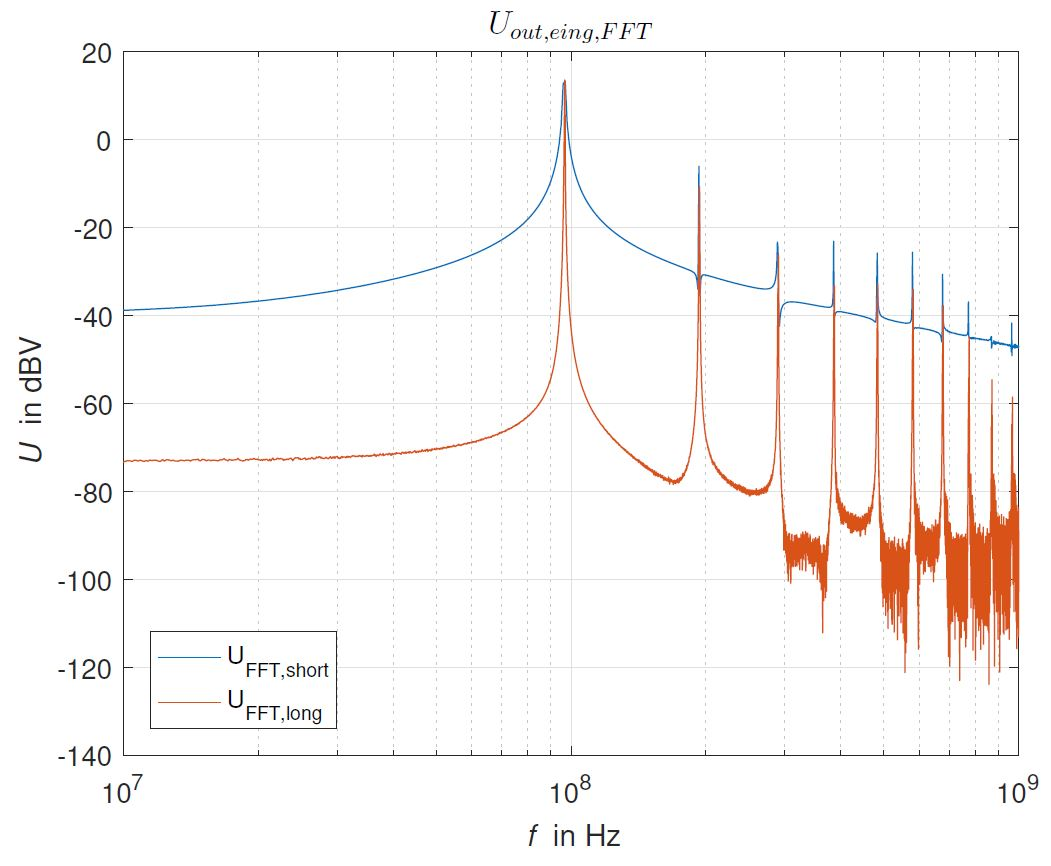
\includegraphics[width = 0.8\textwidth]{\figpath/U_FFT.jpg}
    \caption{FFT der Ausgangsspannung ohne Einschwingvorgang}
    \label{fig_Kap2_07:FFT}
\end{figure}

Mithilfe der Vergrößerung um den Resonanzbereich kann nun die Bandbreite und der Gütefaktor des Oszillators bestimmt werden. Der Zusammenhang des Gütefaktors $Q$, der Resonanzfrequenz $f_0$ und der 3dB-Bandbreite $B$ lautet folgendermaßen:

\begin{equation}
    Q = \frac{f_0}{B}
\end{equation}

Der in Abb. gezeigte Ausschnitt der FFT aus LTSpice soll nun dazu dienen, die gewünschten Größen abzulesen.

\begin{equation*}
    f_0 = \SI{95}{\mega\hertz}
\end{equation*}

\begin{equation*}
    B = f_2 - f_1 = \SI{95.36}{\mega\hertz} - \SI{94.66}{\mega\hertz} = \SI{0.7}{\mega\hertz}
\end{equation*}

\begin{equation*}
    Q = \frac{f_0}{B} = \frac{95}{0.7} = 135.7
\end{equation*}

\begin{figure}[H]
    \centering
    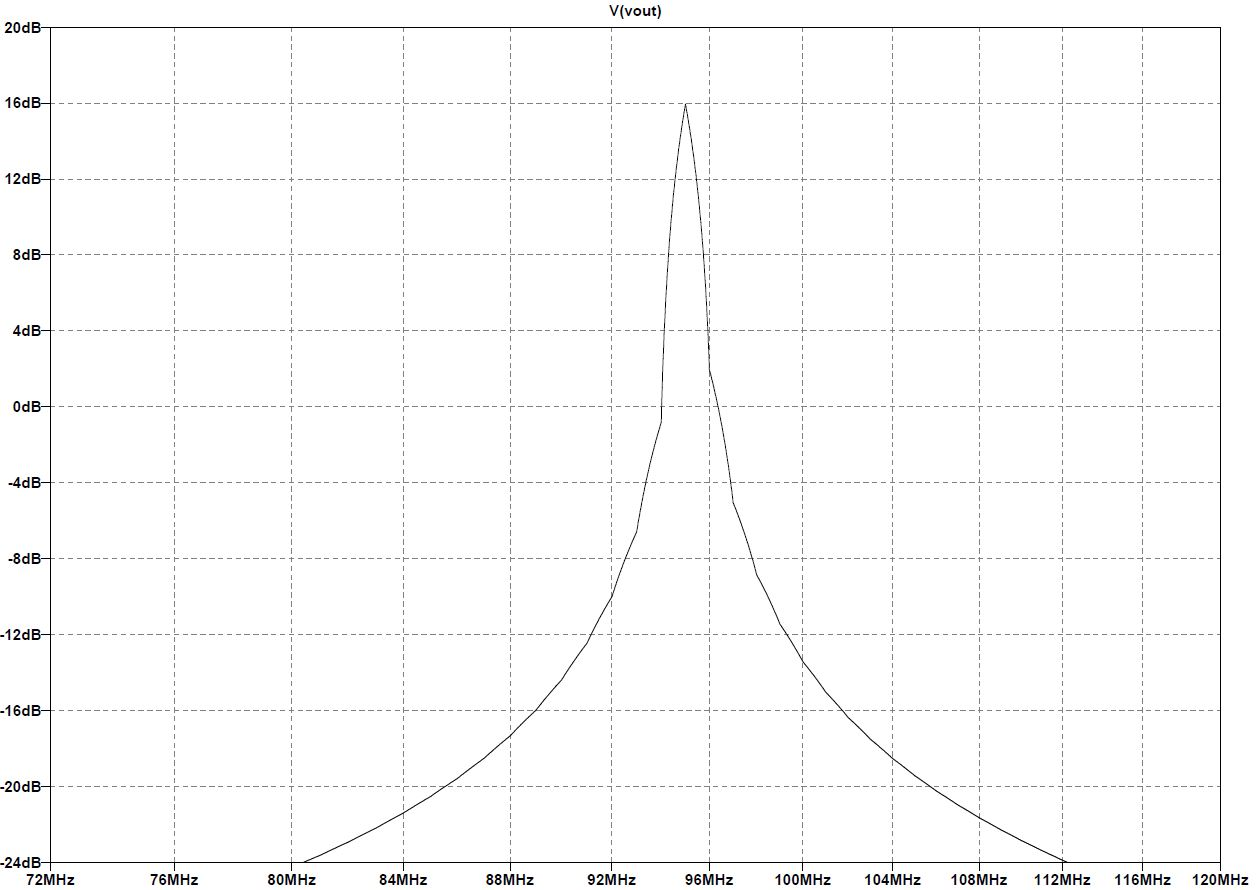
\includegraphics[width = 0.8\textwidth]{\figpath/Oszi_fft_zoom_4.jpg}
    \caption{Vergrößerung der FFT um die Resonanzfrequenz}
    \label{fig_Kap2_05:LTSpiceSchematic}
\end{figure}

\begin{figure}[H]
    \centering
    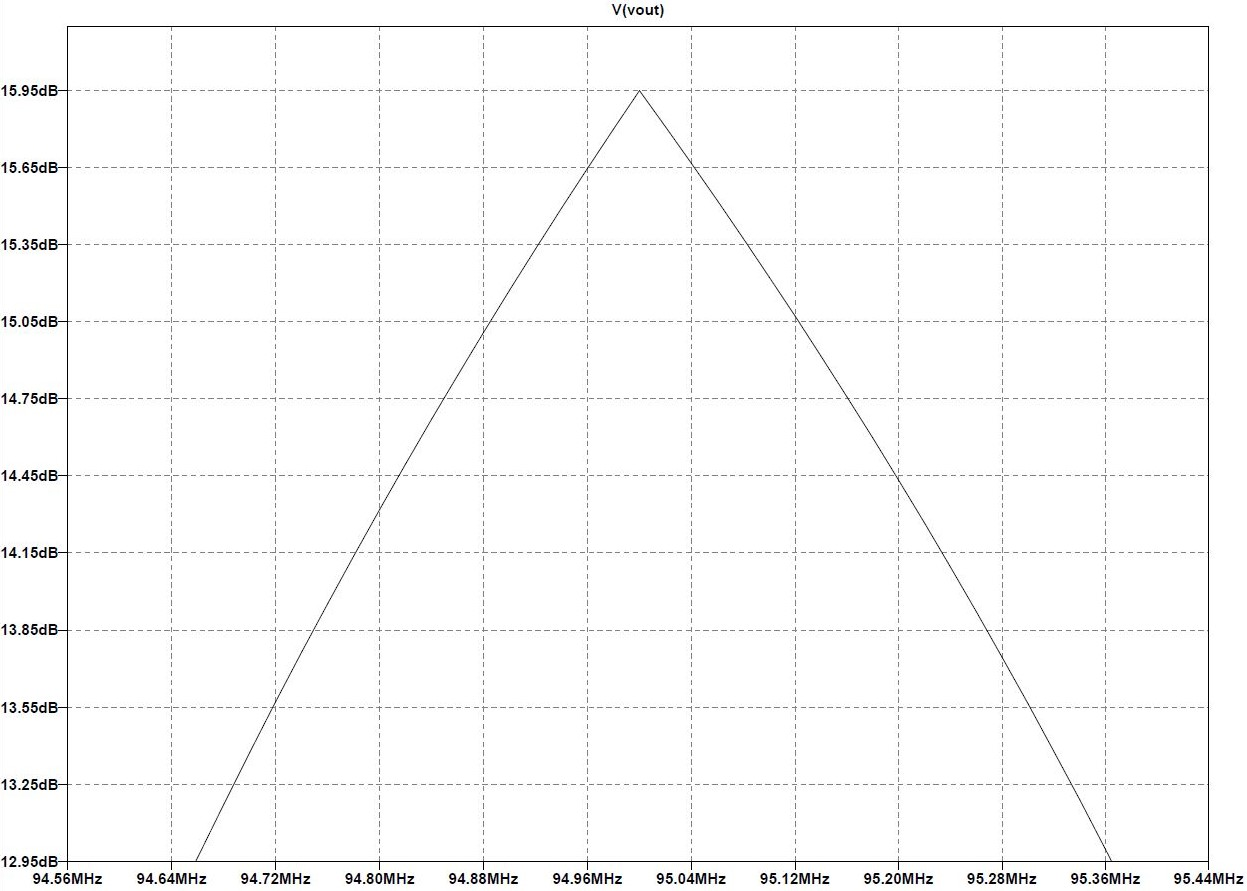
\includegraphics[width = 0.8\textwidth]{\figpath/Oszi_fft_zoom_1.jpg}
    \caption{Vergrößerung der FFT um die Resonanzfrequenz}
    \label{fig_Kap2_05:LTSpiceSchematic}
\end{figure}

Im nächsten Schritt wurde die Simulationszeit von $\SI{2}{\micro\second}$ auf $\SI{10}{\micro\second}$ erhöht, der Einschwingvorgang wurde wiederum nach $\SI{1}{\micro\second}$ weggeschnitten und vom eingeschwungenen Zustand die FFT berechnet. Von außen betrachtet ähneln sich die Fouriertransformierten beider Simulationsvarianten stark, vergrößert man jedoch die Ansicht um die Resonanzfrequenz erkennt man Unterschiede. Die Resonanzfrequenz hat sich etwas nach oben verschoben. Die 3dB-Bandbreite um die Resonanzfrequenz ist schmaler ausgeprägt, was in einem höheren Gütefaktor resultiert.

\begin{figure}[H]
    \centering
    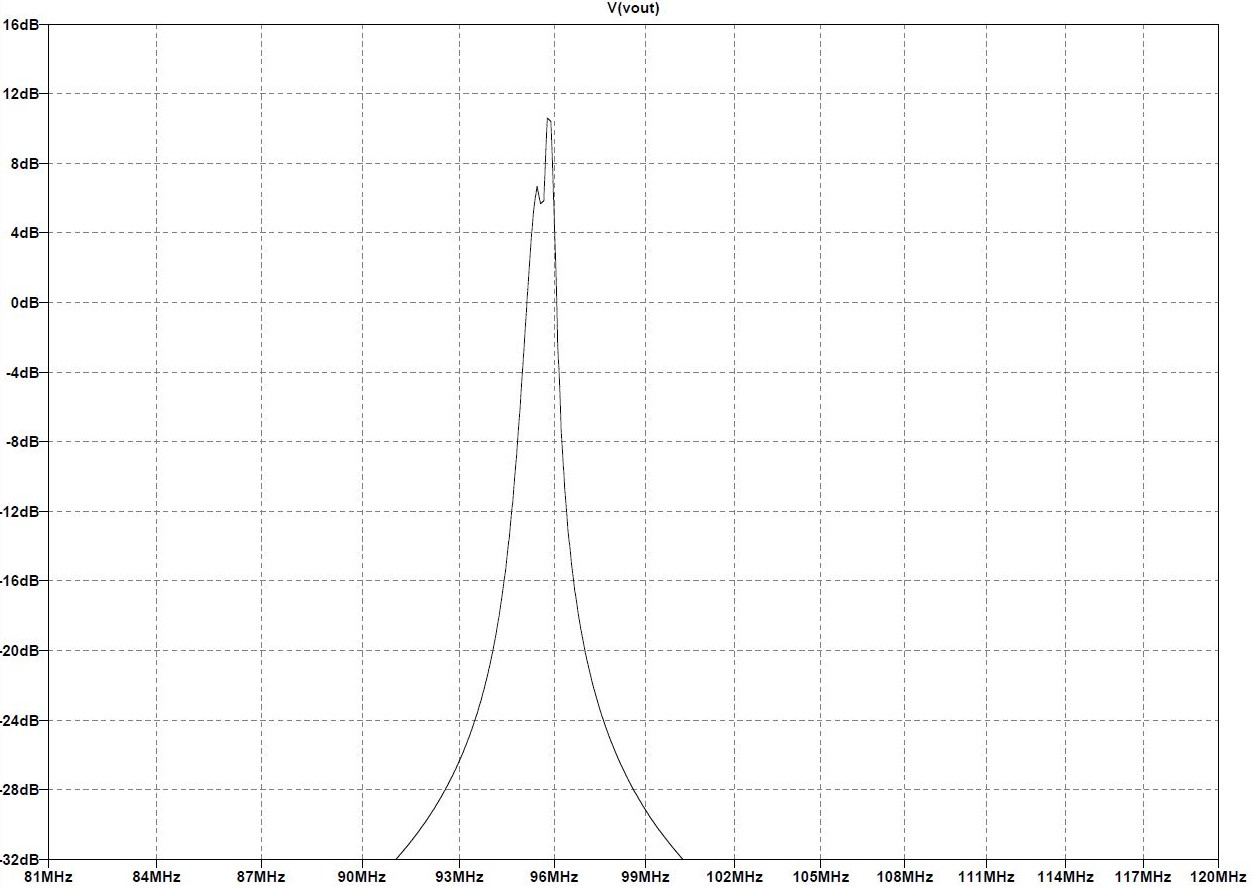
\includegraphics[width = 0.8\textwidth]{\figpath/Oszi_fft_zoom_2.jpg}
    \caption{Vergrößerung der FFT um die Resonanzfrequenz}
    \label{fig_Kap2_05:LTSpiceSchematic}
\end{figure}

\begin{figure}[H]
    \centering
    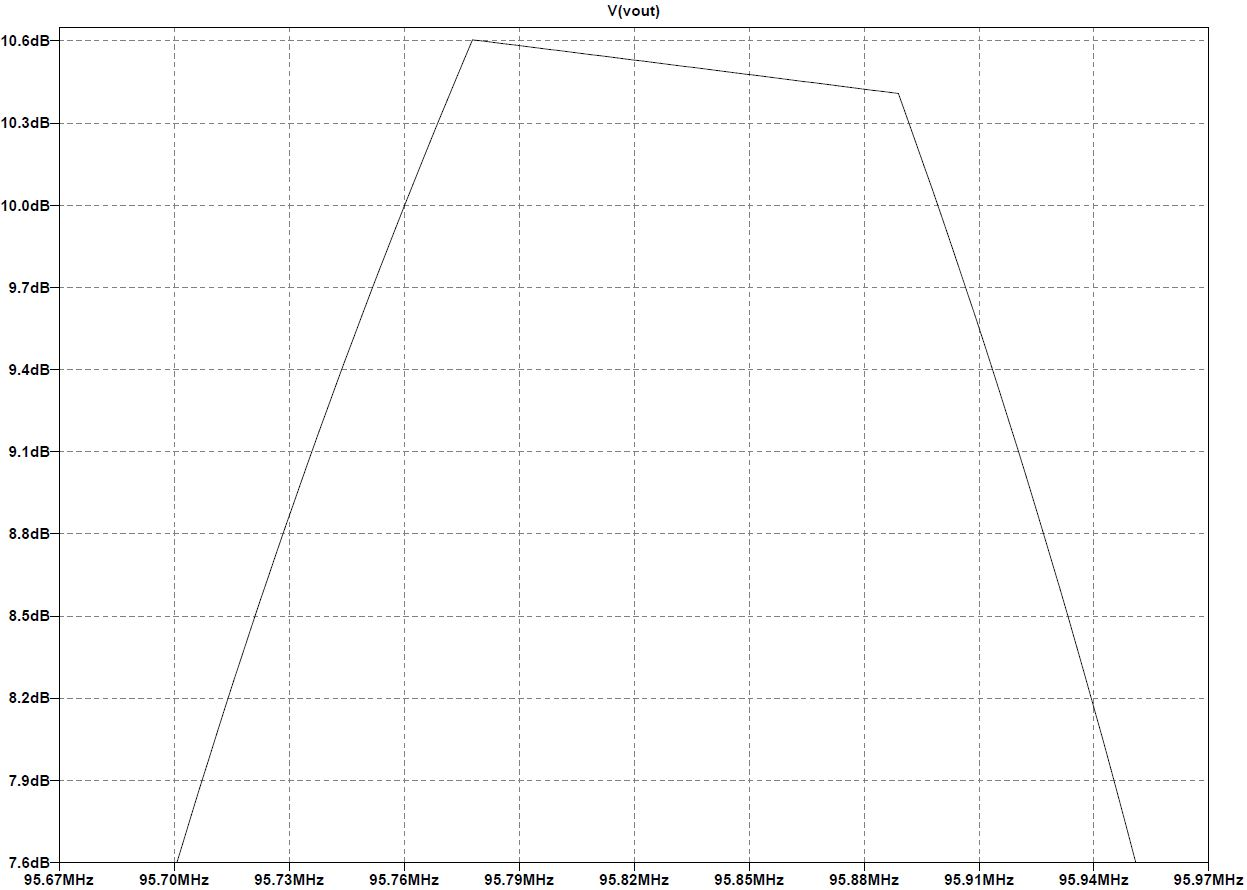
\includegraphics[width = 0.8\textwidth]{\figpath/Oszi_fft_zoom_3.jpg}
    \caption{Vergrößerung der FFT um die Resonanzfrequenz}
    \label{fig_Kap2_05:LTSpiceSchematic}
\end{figure}

\begin{equation*}
    f_0 = \SI{95.8}{\mega\hertz}
\end{equation*}

\begin{equation*}
    B = f_2 - f_1 =  = \SI{95.95}{\mega\hertz} - \SI{95.7}{\mega\hertz} = \SI{0.25}{\mega\hertz}
\end{equation*}

\begin{equation}
    Q = \frac{f_0}{B} = \frac{95.8}{0.25} = 383.2
\end{equation}

Als nächstes wird die Abhängigkeit der Resonanzfrequenz vom Arbeitspunkt des Transistors untersucht. Hierzu wurde der Widerstand $R_1$ variiert und über Simulation die Resonanzfrequen ermittelt. Die Werte wurden in Tab. eingetragen sowie als Diagramm in Abb. \ref{fig_Kap2_09:AP} dargestellt.

\begin{table}[H]
\centering
\begin{tabular}{|c|c|c|} \hline
$R_1$ in k$\Omega$ & $U_L$ in V & $f_0$ im MHz \\ \hline
27 & 0.596 & 96.5 \\ \hline
15 & 0.628 & 96 \\ \hline
10 & 0.642 & 95.5 \\ \hline
2.7 & 0.674 & 92 \\ \hline
1 & 0.687 & 87.10 \\ \hline
\end{tabular}
\caption{Variation des AP und Resonanzfrequenz}
\label{tab_Kap2_02:AP} 
\end{table}

\begin{figure}[H]
	\centering \small
	% This file was created by matlab2tikz.
%
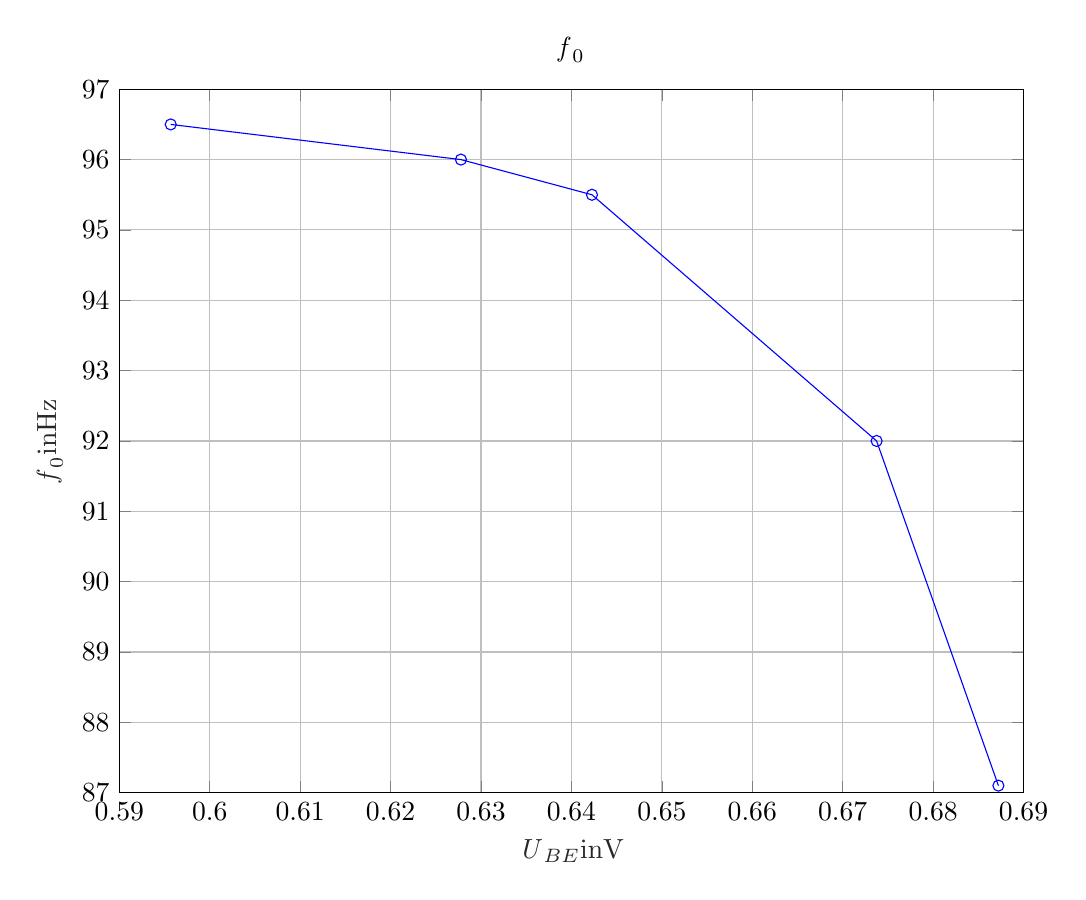
\begin{tikzpicture}

\begin{axis}[%
width=4.521in,
height=3.517in,
at={(0.758in,0.519in)},
scale only axis,
xmin=0.59,
xmax=0.69,
xlabel style={font=\color{white!15!black}},
xlabel={$\text{\it{} U}_{\text{BE}}\text{ \rm{} in V}$},
ymin=87,
ymax=97,
ylabel style={font=\color{white!15!black}},
ylabel={$\text{\it{} f}_\text{0}\text{ \rm{} in Hz}$},
axis background/.style={fill=white},
title style={font=\bfseries},
title={$\text{\it{} f}_{\text{0}}$},
xmajorgrids,
ymajorgrids
]
\addplot [color=blue, mark=o, mark options={solid, blue}, forget plot]
  table[row sep=crcr]{%
0.68722	87.1\\
0.67375	92\\
0.64227	95.5\\
0.627778	96\\
0.595685	96.5\\
};
\end{axis}
\end{tikzpicture}%
	\caption{$f_0$ in Abhängigkeit des AP}
	\label{fig_Kap2_09:AP}
\end{figure}



